\documentclass[draft,sw]{agutexSI2019}

\usepackage{graphicx}
\setkeys{Gin}{draft=false}


\begin{document}

\title{Deep Neural Network for SYM-H Forecasting aided by ACE's SWICS plasma data}

\authors{Armando Collado-Villaverde\affil{1}, Pablo Mu\~noz\affil{1}, Consuelo Cid\affil{2}}

\affiliation{1}{Department of Computer Engineering, University of Alcal\'a, Alcal\'a de Henares, Madrid, Spain}
\affiliation{2}{Department of Physics and Mathematics, University of Alcal\'a, Alcal\'a de Henares, Madrid, Spain}

\begin{article}

\renewcommand\tablename{Figure}

\noindent\textbf{Contents of this file}
\begin{enumerate}
\item Figures S1 to S17
\end{enumerate}

\noindent\textbf{Introduction}

This file contains the figures for each of the test geomagnetic storms, comparing the observed and predicted SYM-H for the two trained neural networks for both time horizons, 1 and 2 hours ahead. 

\begin{itemize}
    \item 1 hour SWEPAM model in real-time: Model trained on SWEPAM data only and evaluated in real-time conditions, SWEPAM's missing data will be interpolated if the value to interpolate to is available, otherwise the last valid value is propagated for 1 hour ahead forecasts.
    \item 2 hours SWEPAM model in real-time: Model trained on SWEPAM data only and evaluated in real-time conditions, SWEPAM's missing data will be interpolated if the value to interpolate to is available, otherwise the last valid value is propagated for 1 hour ahead forecasts.
    \item 1 hour SWICS model in real-time: Model trained with SWEPAM's missing data filled using SWICS evaluated in real-time conditions, SWEPAM's missing data will be interpolated if the value to interpolate to is available, otherwise the last valid value is propagated for 1 hour ahead forecasts.
    \item 2 hours SWICS model in real-time: Model trained with SWEPAM's missing data filled using SWICS evaluated in real-time conditions, SWEPAM's missing data will be interpolated if the value to interpolate to is available, otherwise the last valid value is propagated for 2 hours ahead forecasts.
	\item Laboratory conditions SWICS model 1h: Model trained with SWEPAM's missing data filled using SWICS and evaluated in the same conditions for 1 hour ahead forecasts.
    \item Laboratory conditions SWICS model 2h: Model trained with SWEPAM's missing data filled using SWICS and evaluated in the same conditions for 2 hours ahead forecasts.

    
\end{itemize}


\end{article}
\clearpage


% Figure for storm 26
\begin{table}
\centering
\begin{tabular}{cc}
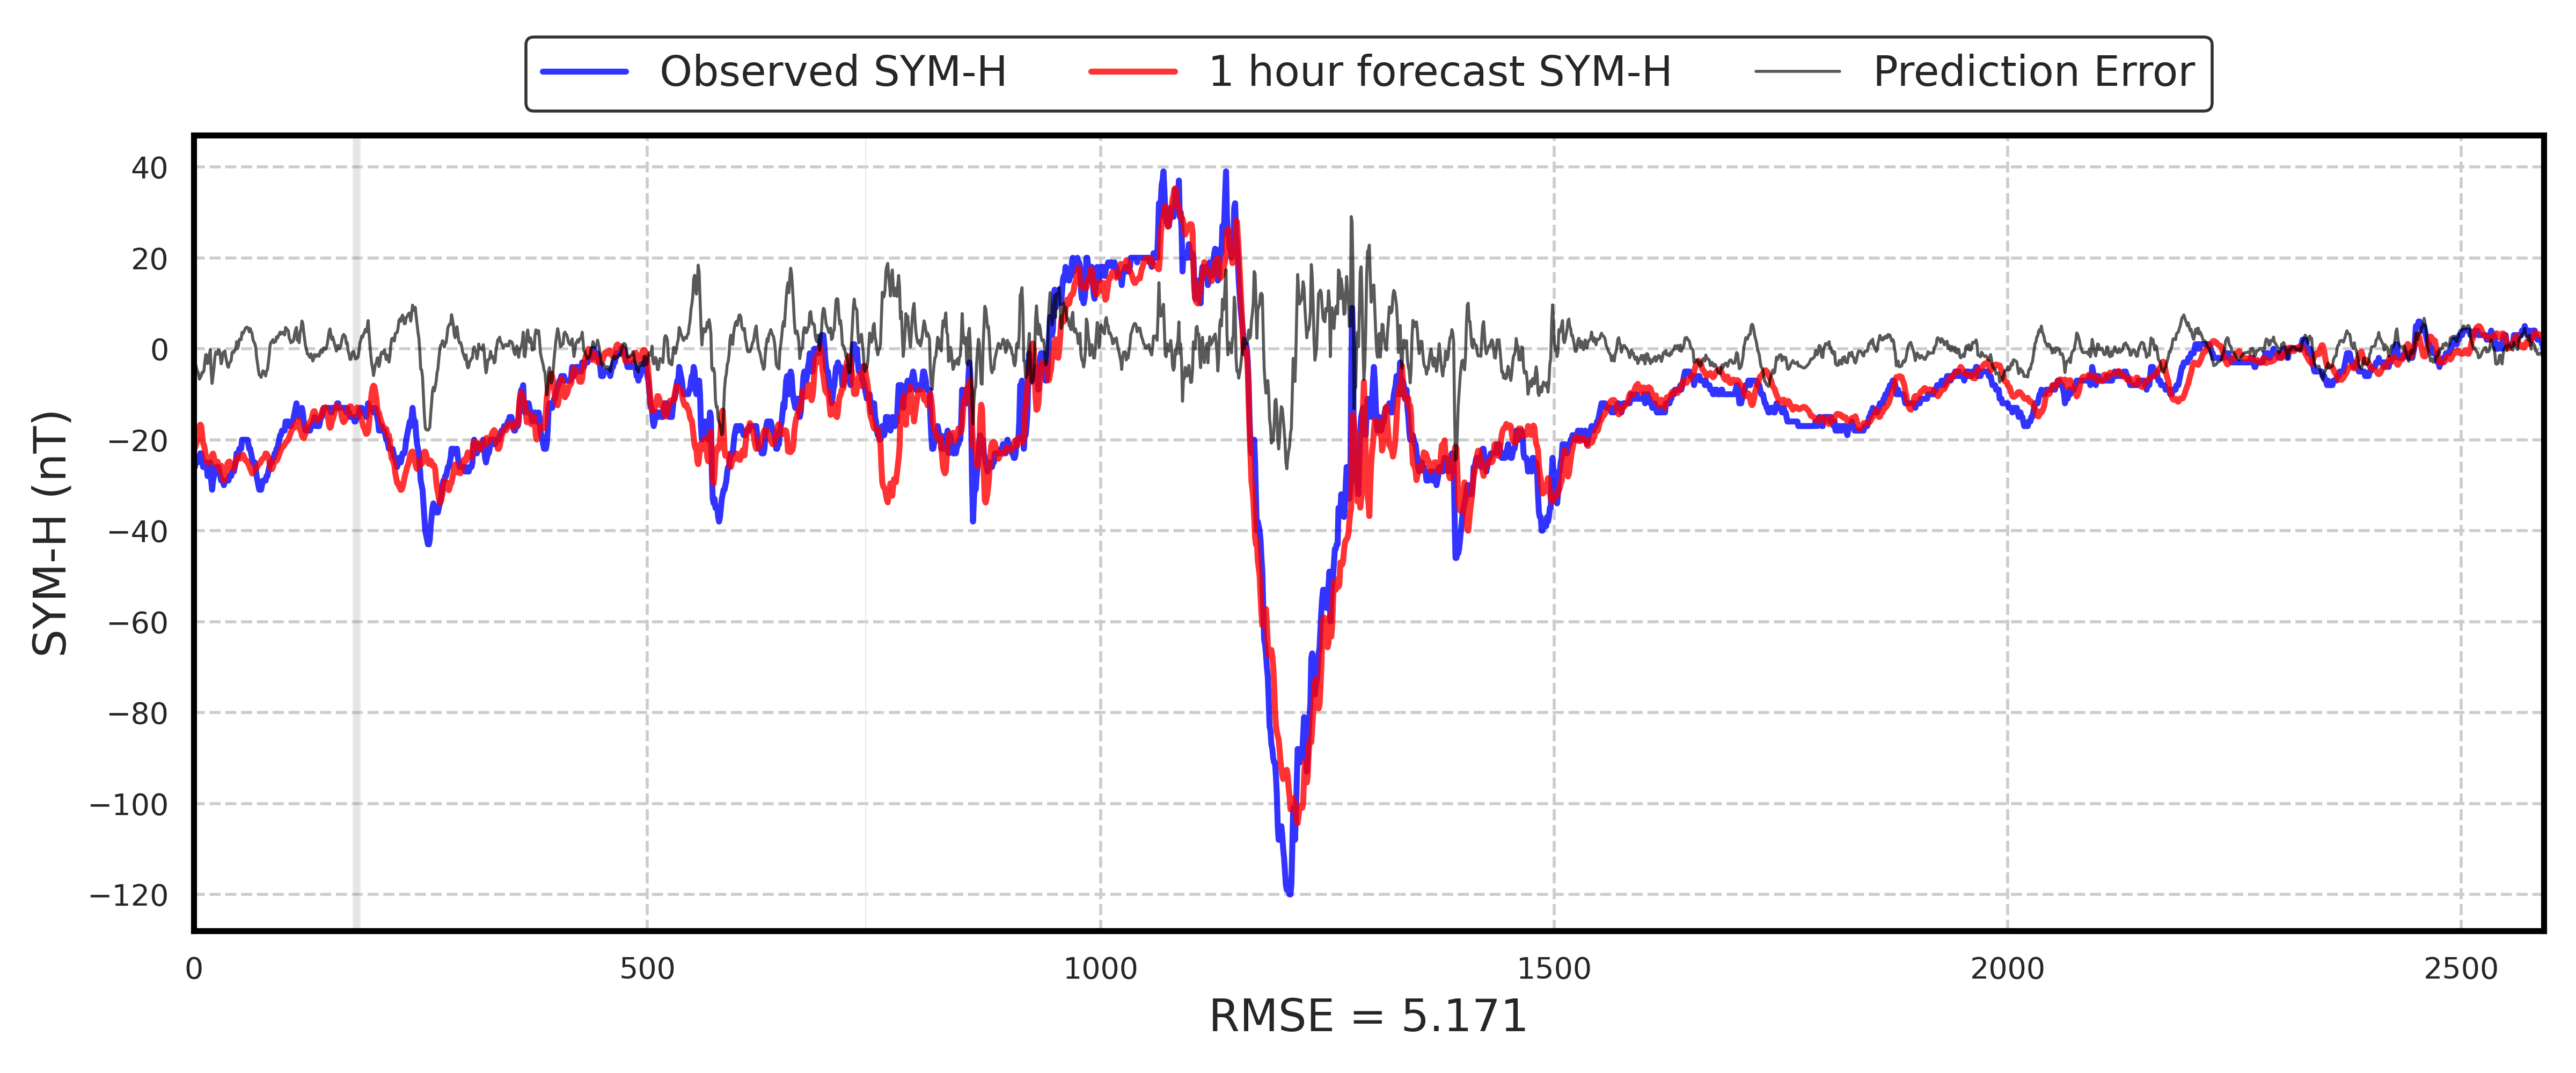
\includegraphics[width=0.49\linewidth]{paper_plots_shade/1h_swics/1h_swics_storm_26.png}
&
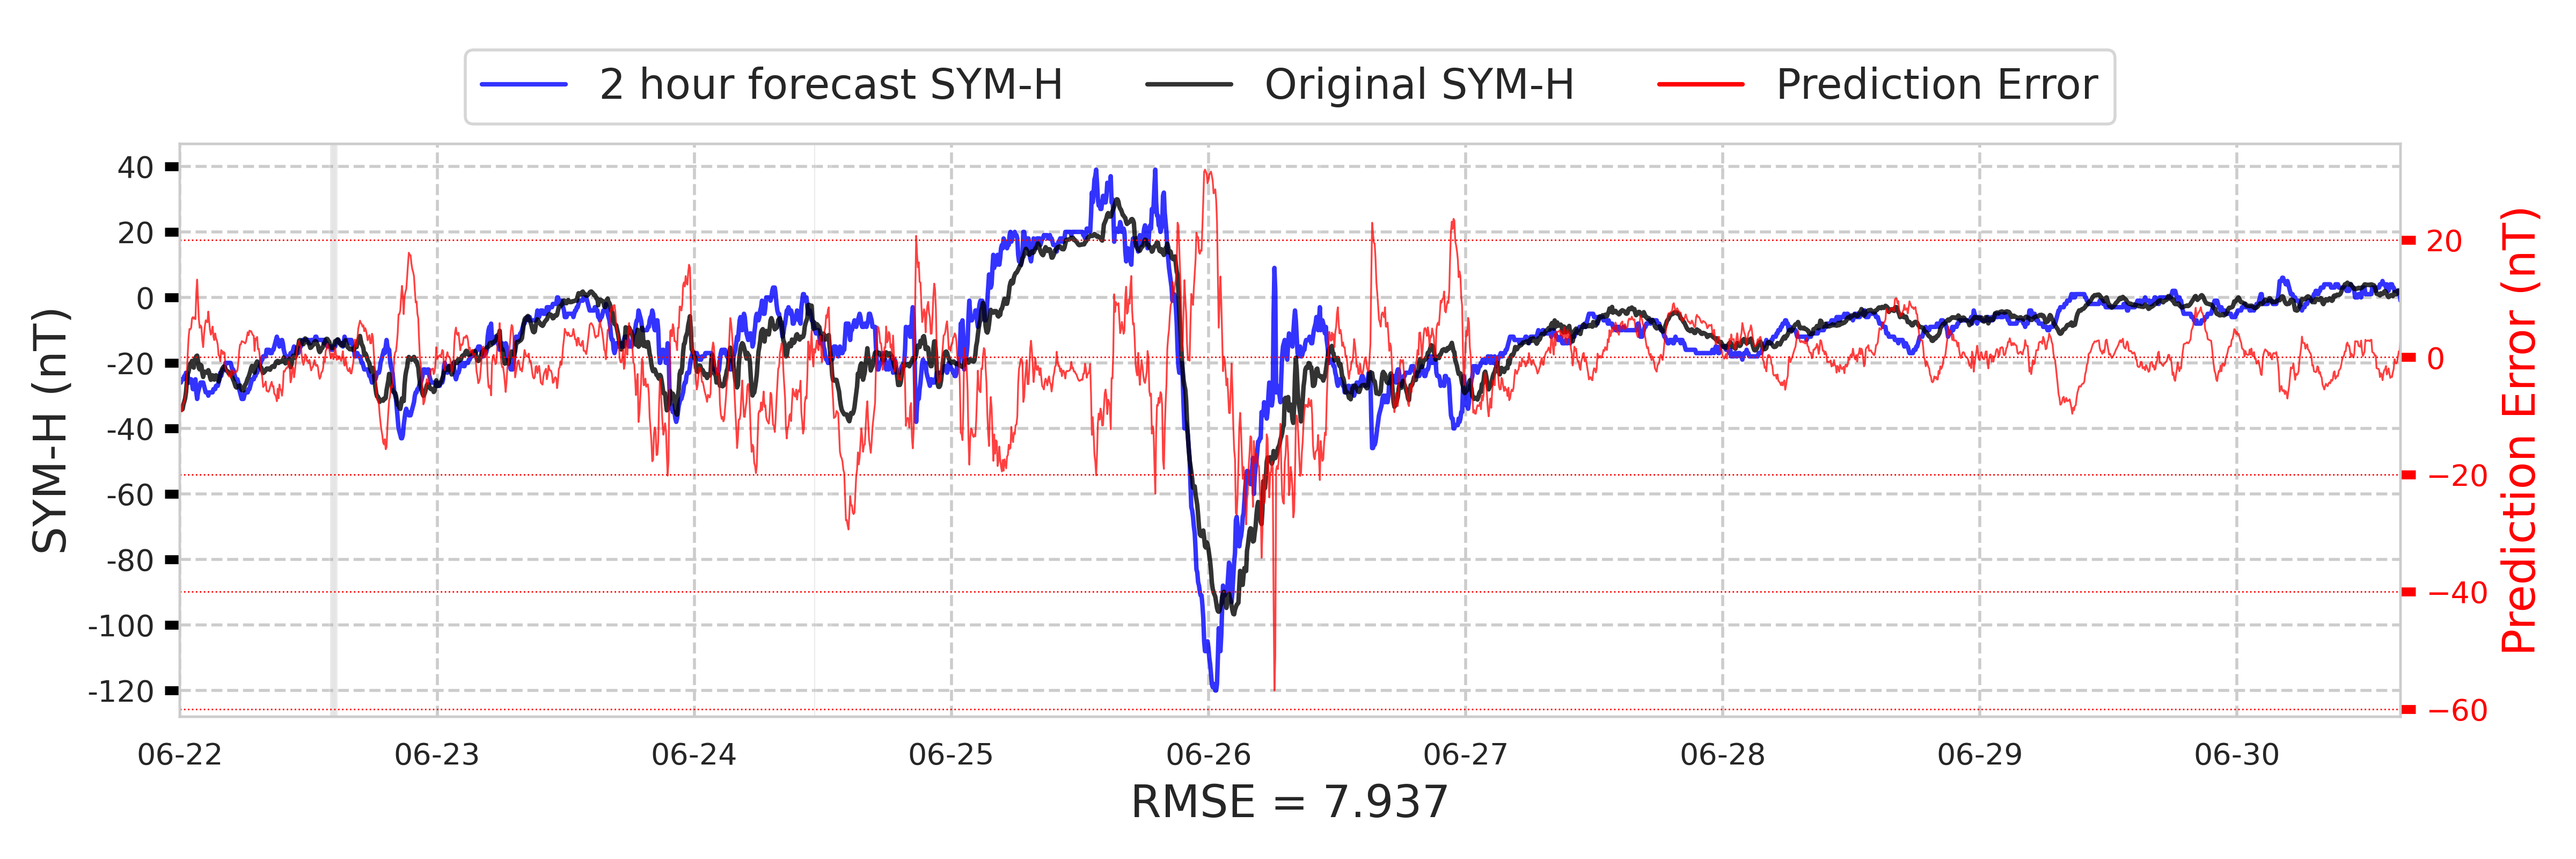
\includegraphics[width=0.49\linewidth]{paper_plots_shade/2h_swics/2h_swics_storm_26.png}
\\
\shortstack{1h forecast using SWICS\\ in laboratory conditions} & \shortstack{2h forecast using SWICS\\ in laboratory conditions}
\vspace*{12pt}
\\
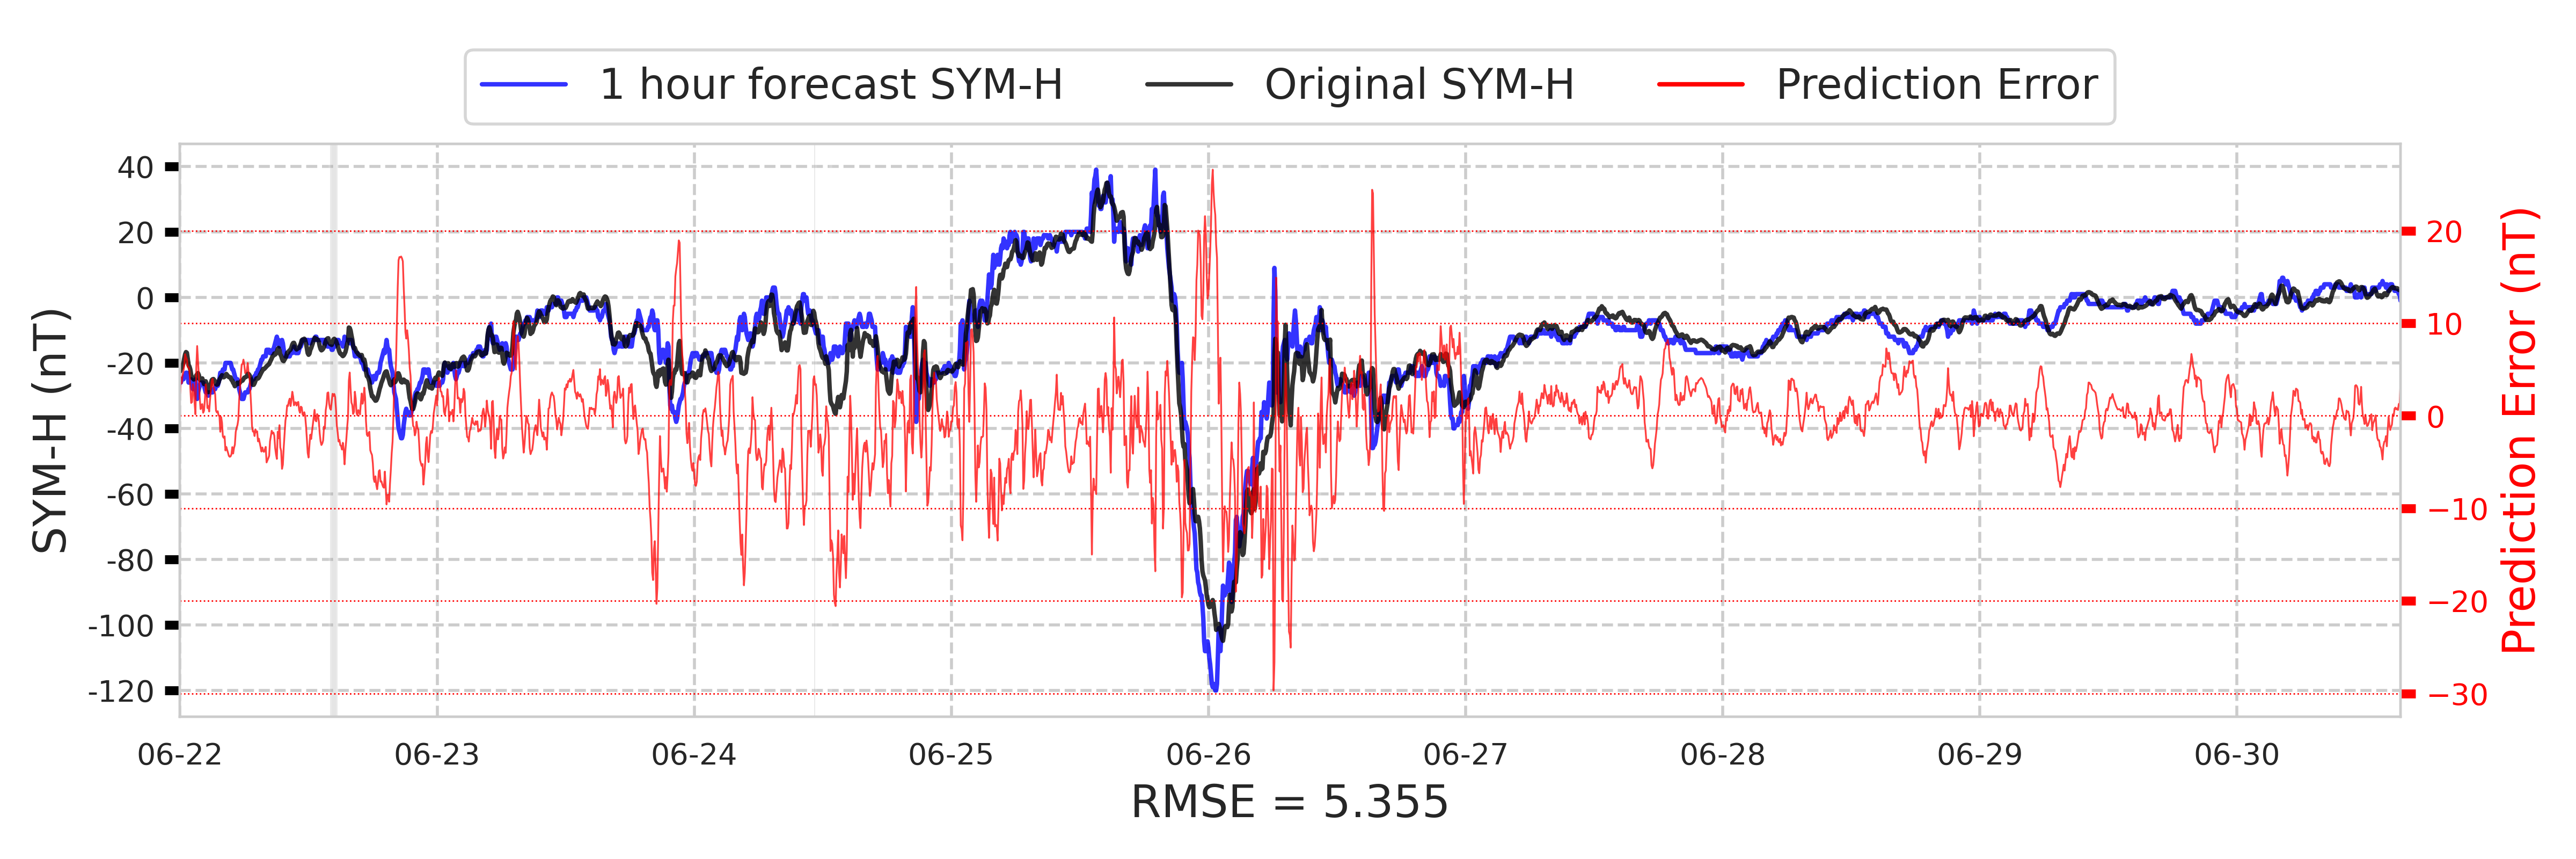
\includegraphics[width=0.49\linewidth]{paper_plots_shade/1h_swics_rt/1h_swics_rt_storm_26.png}
&
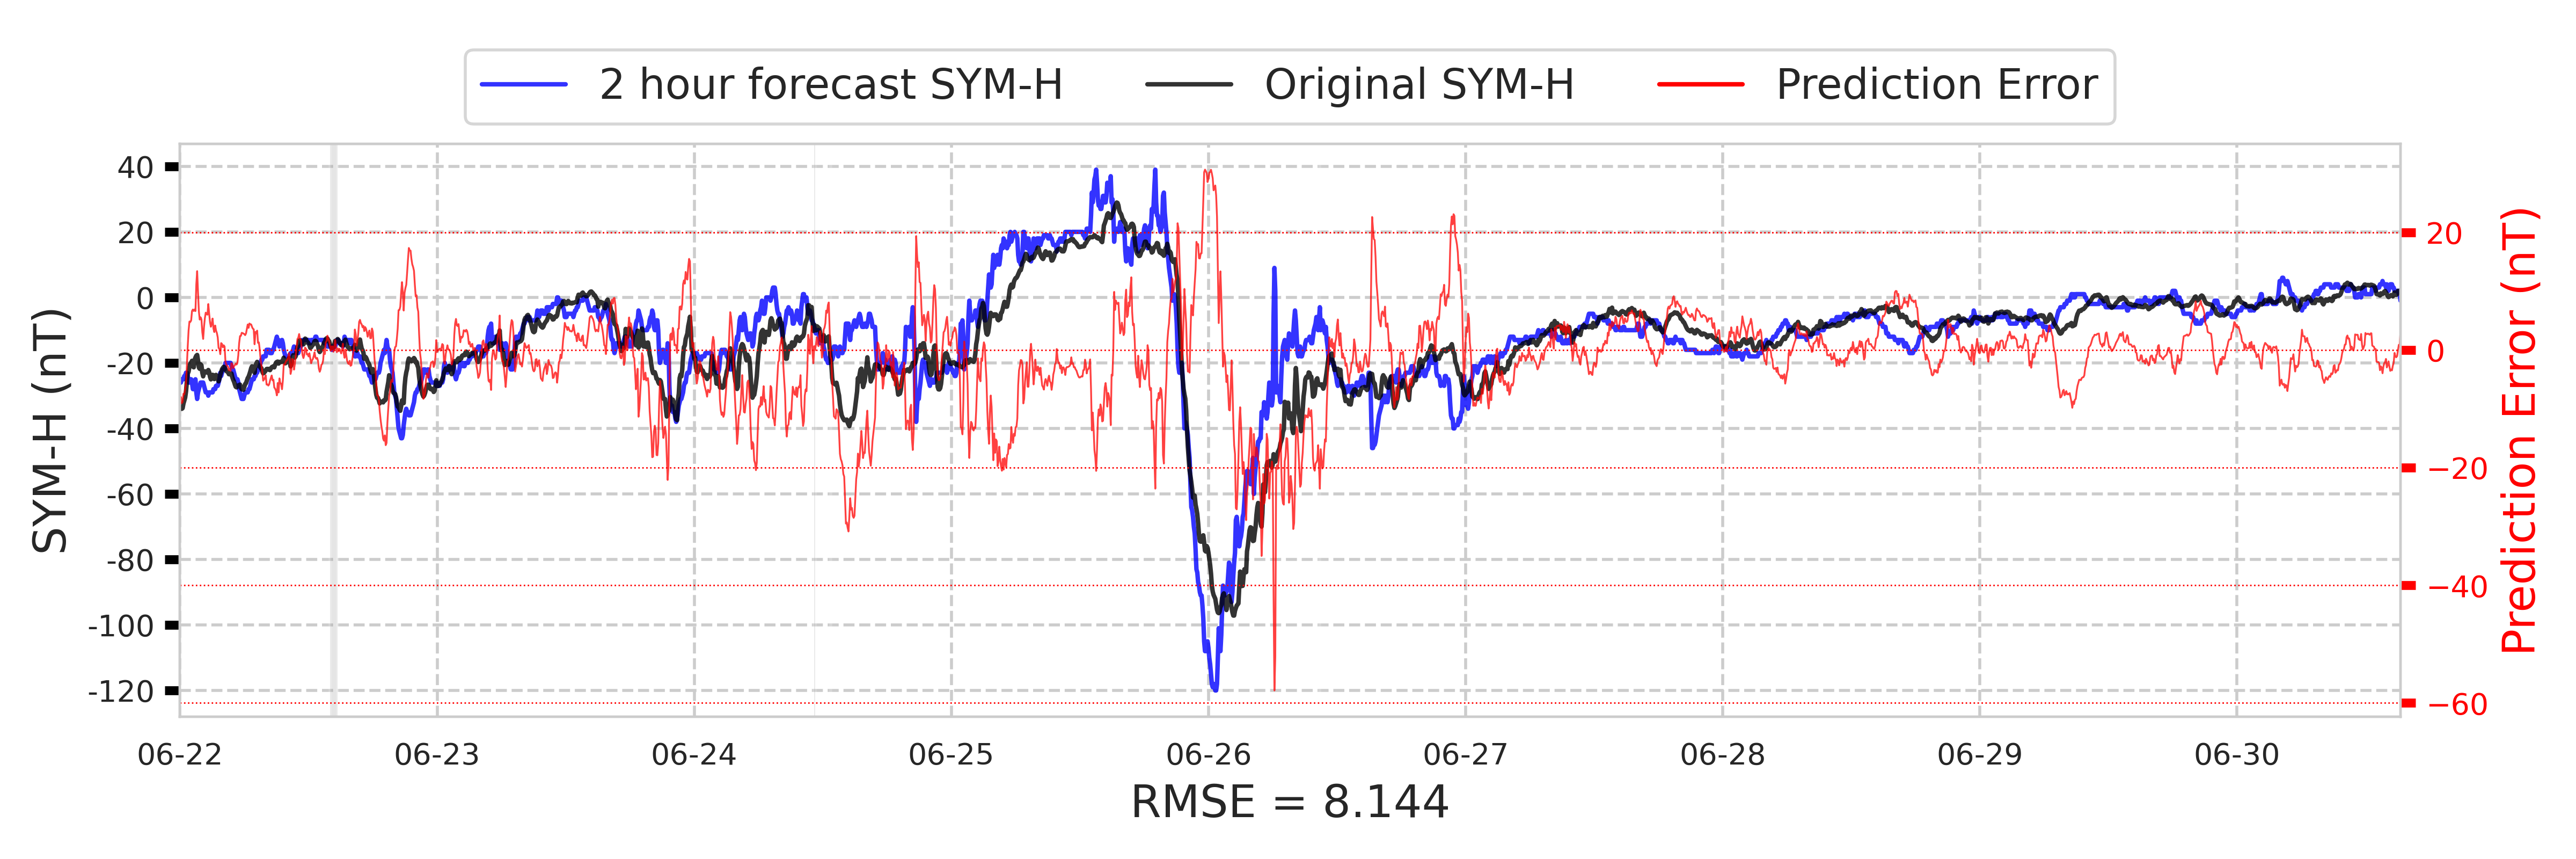
\includegraphics[width=0.49\linewidth]{paper_plots_shade/2h_swics_rt/2h_swics_rt_storm_26.png}
\\
\shortstack{1h operational forecast trained\\ with SWEPAM and SWICS data} & \shortstack{2h operational forecast trained\\ with SWEPAM and SWICS data}
\vspace*{12pt}
\\
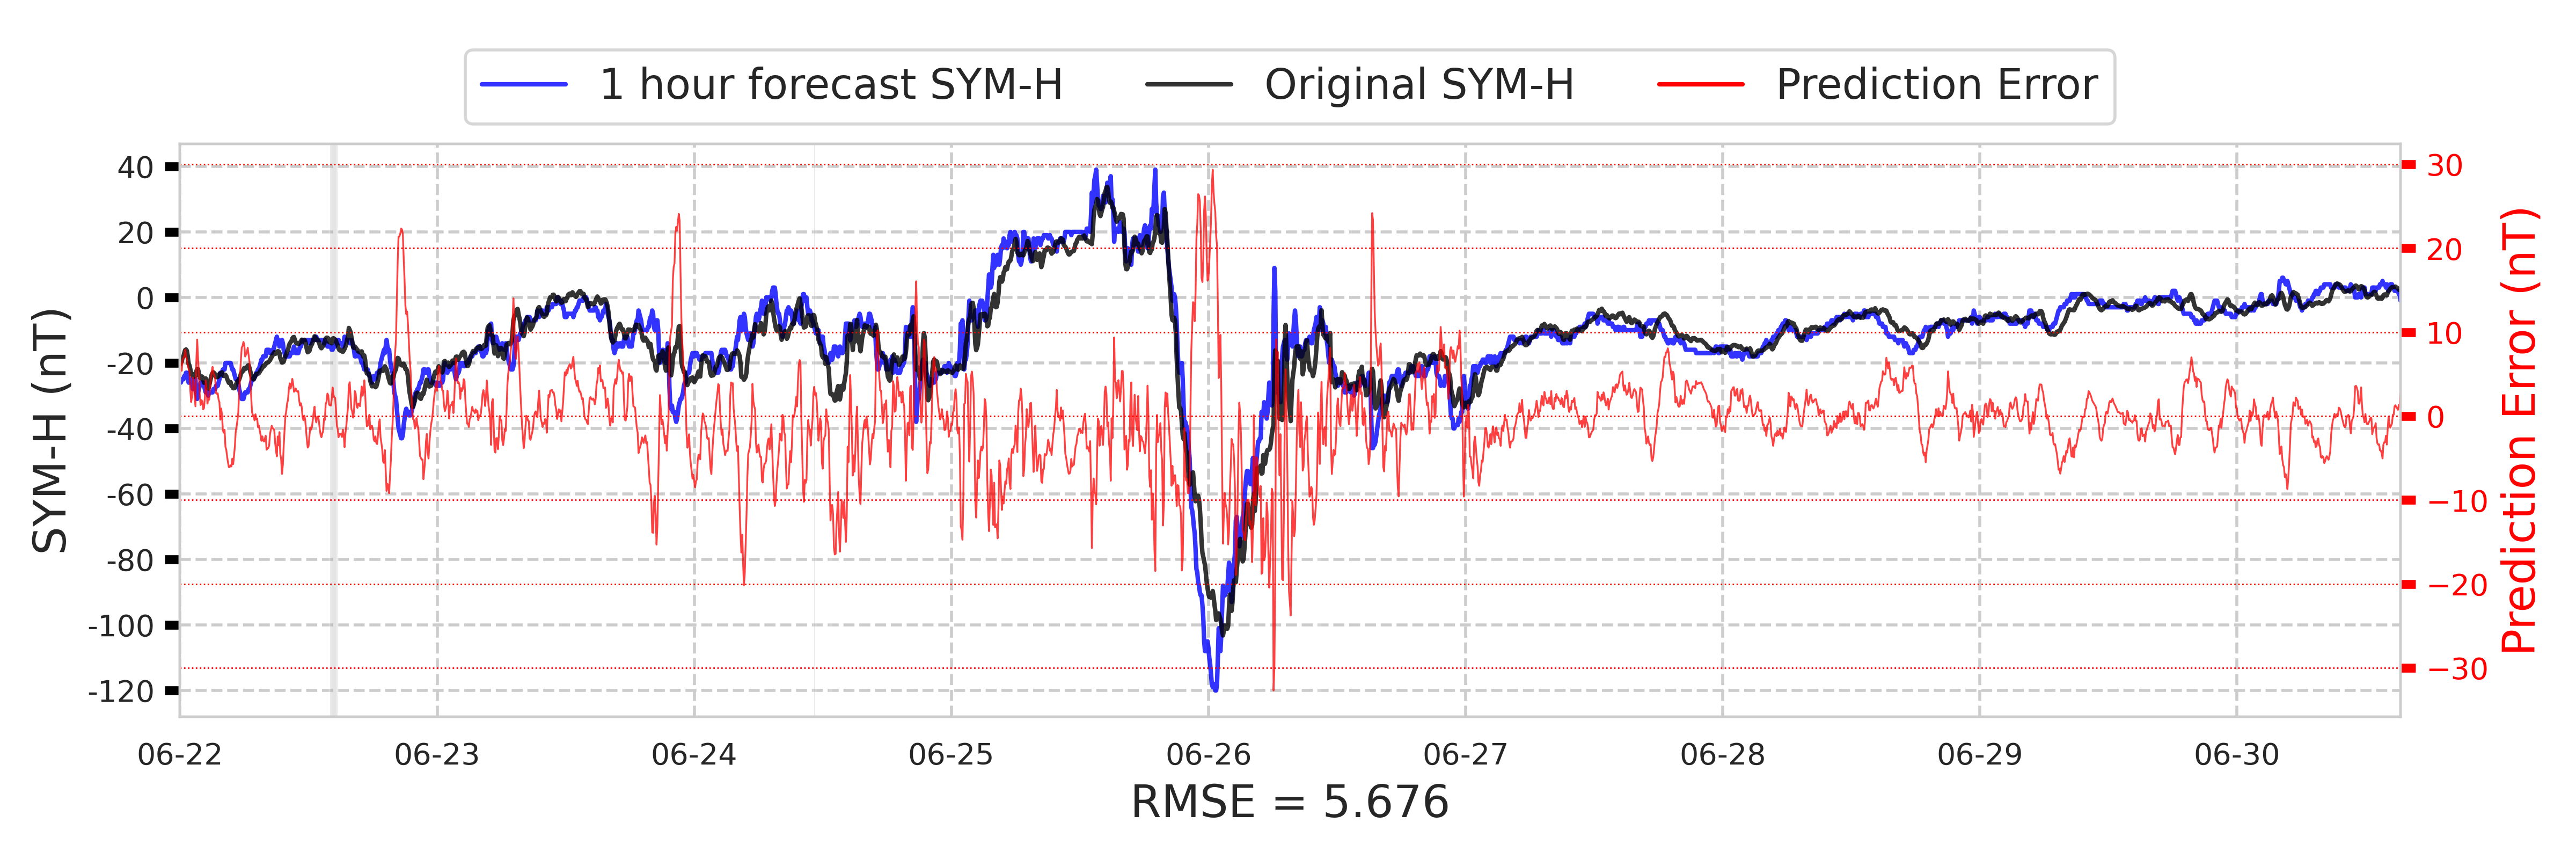
\includegraphics[width=0.49\linewidth]{paper_plots_shade/1h_swepam_rt/1h_swepam_rt_storm_26.png}
&
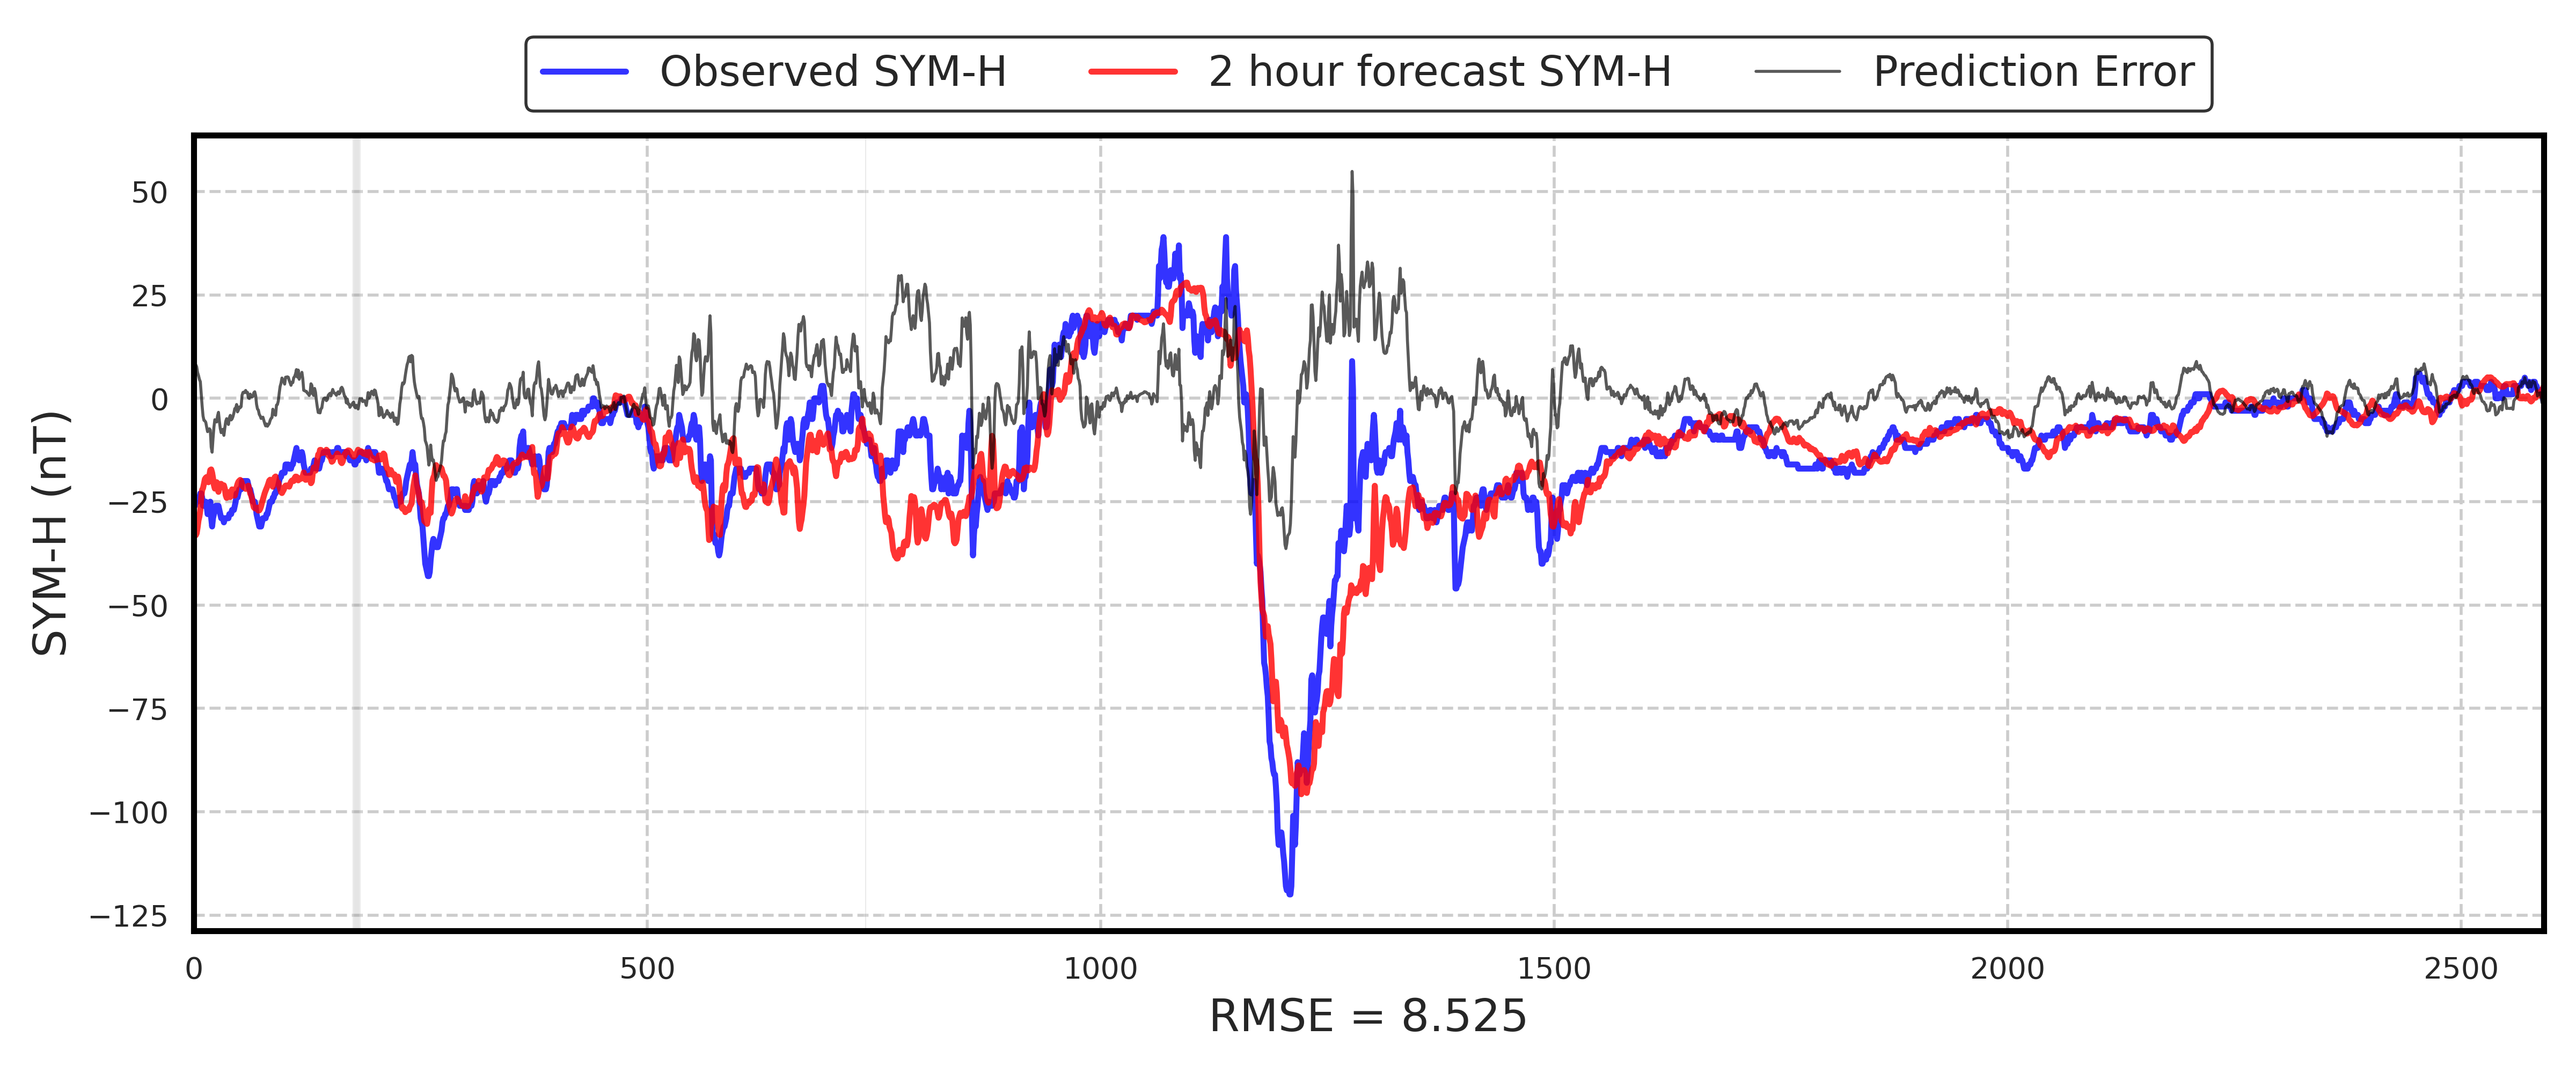
\includegraphics[width=0.49\linewidth]{paper_plots_shade/2h_swepam_rt/2h_swepam_rt_storm_26.png}
\\
\shortstack{1h operational forecast trained\\ with SWEPAM data only} & \shortstack{2h operational forecast trained\\ with SWEPAM data only}
\vspace*{12pt}
\\
\end{tabular}
\caption{Predictions for Storm Number 26 -- June of 1998}
\label{storm-26}
\end{table}



% Figure for storm 27
\begin{table}
\centering
\begin{tabular}{cc}
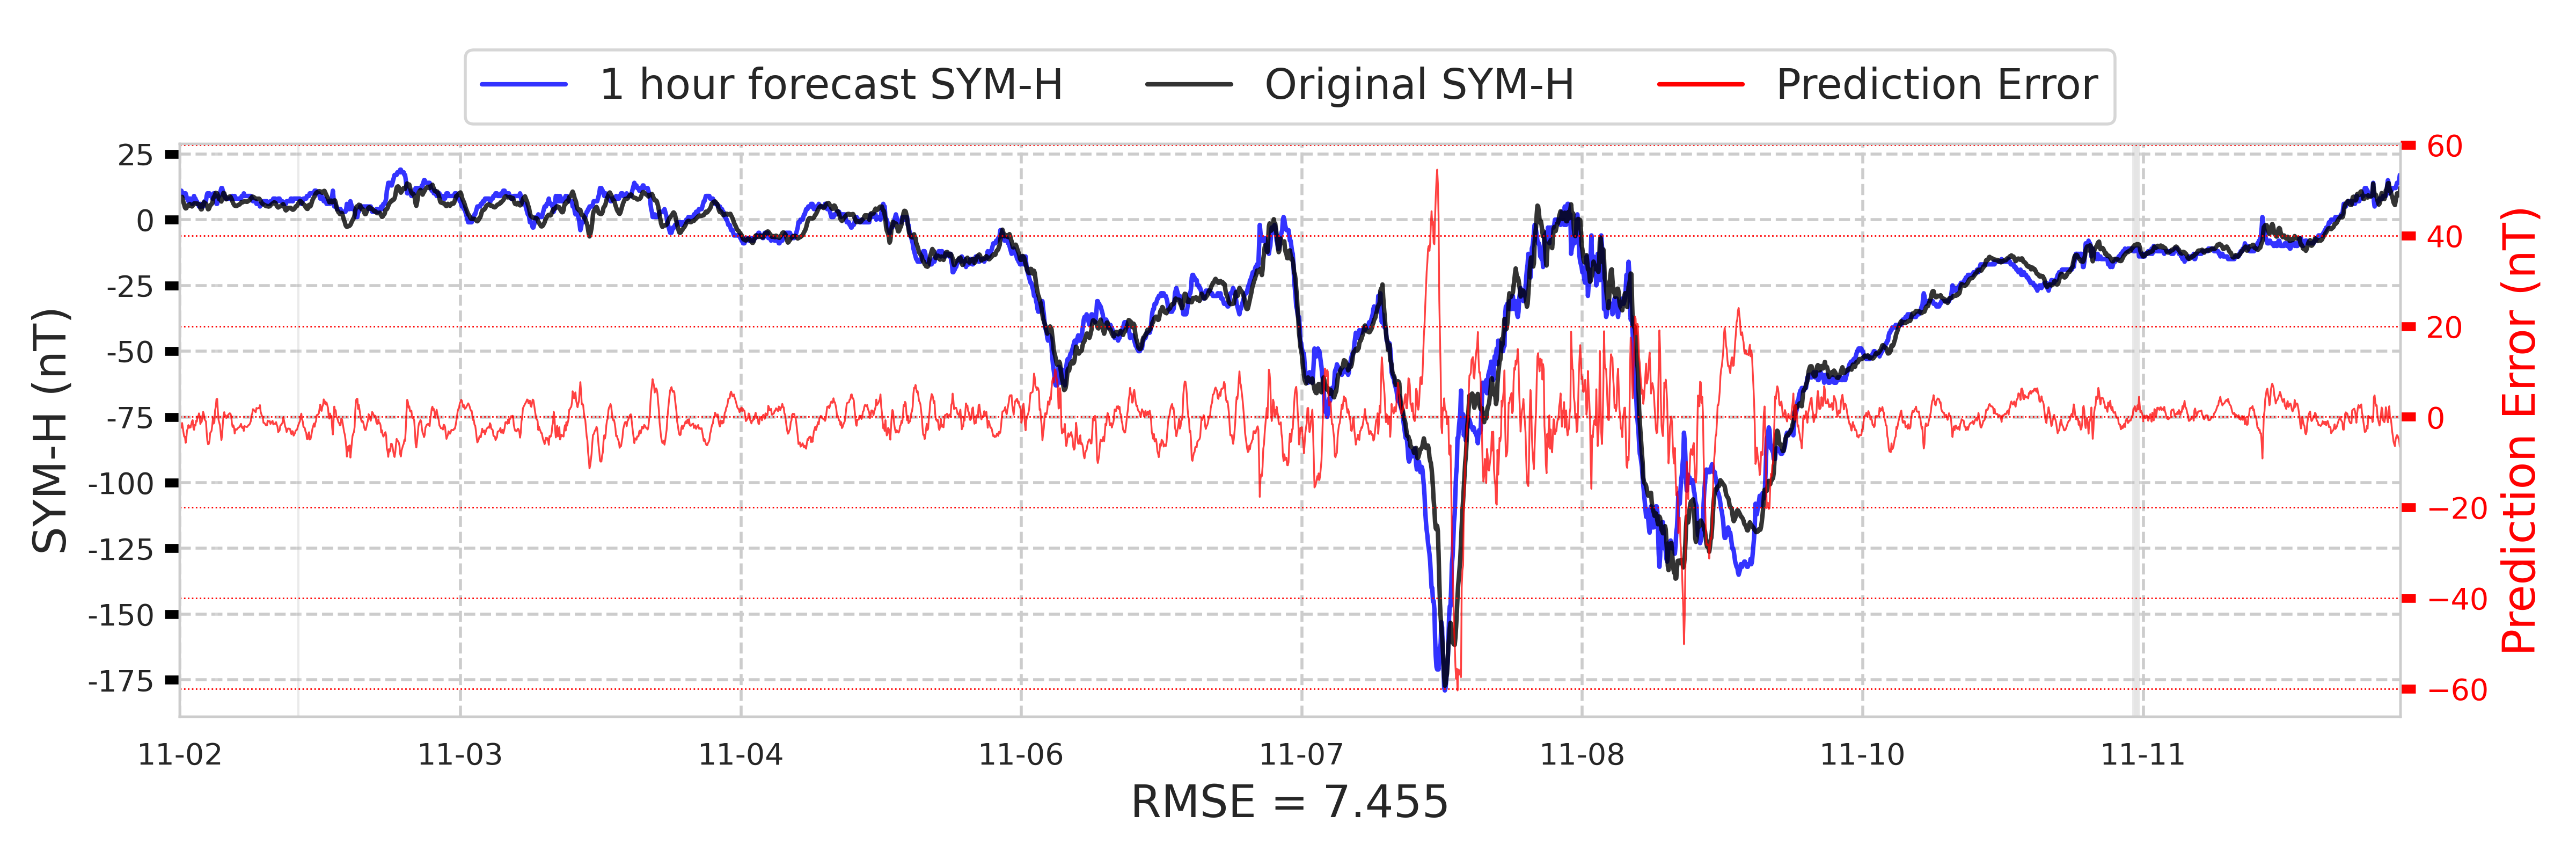
\includegraphics[width=0.49\linewidth]{paper_plots_shade/1h_swics/1h_swics_storm_27.png}
&
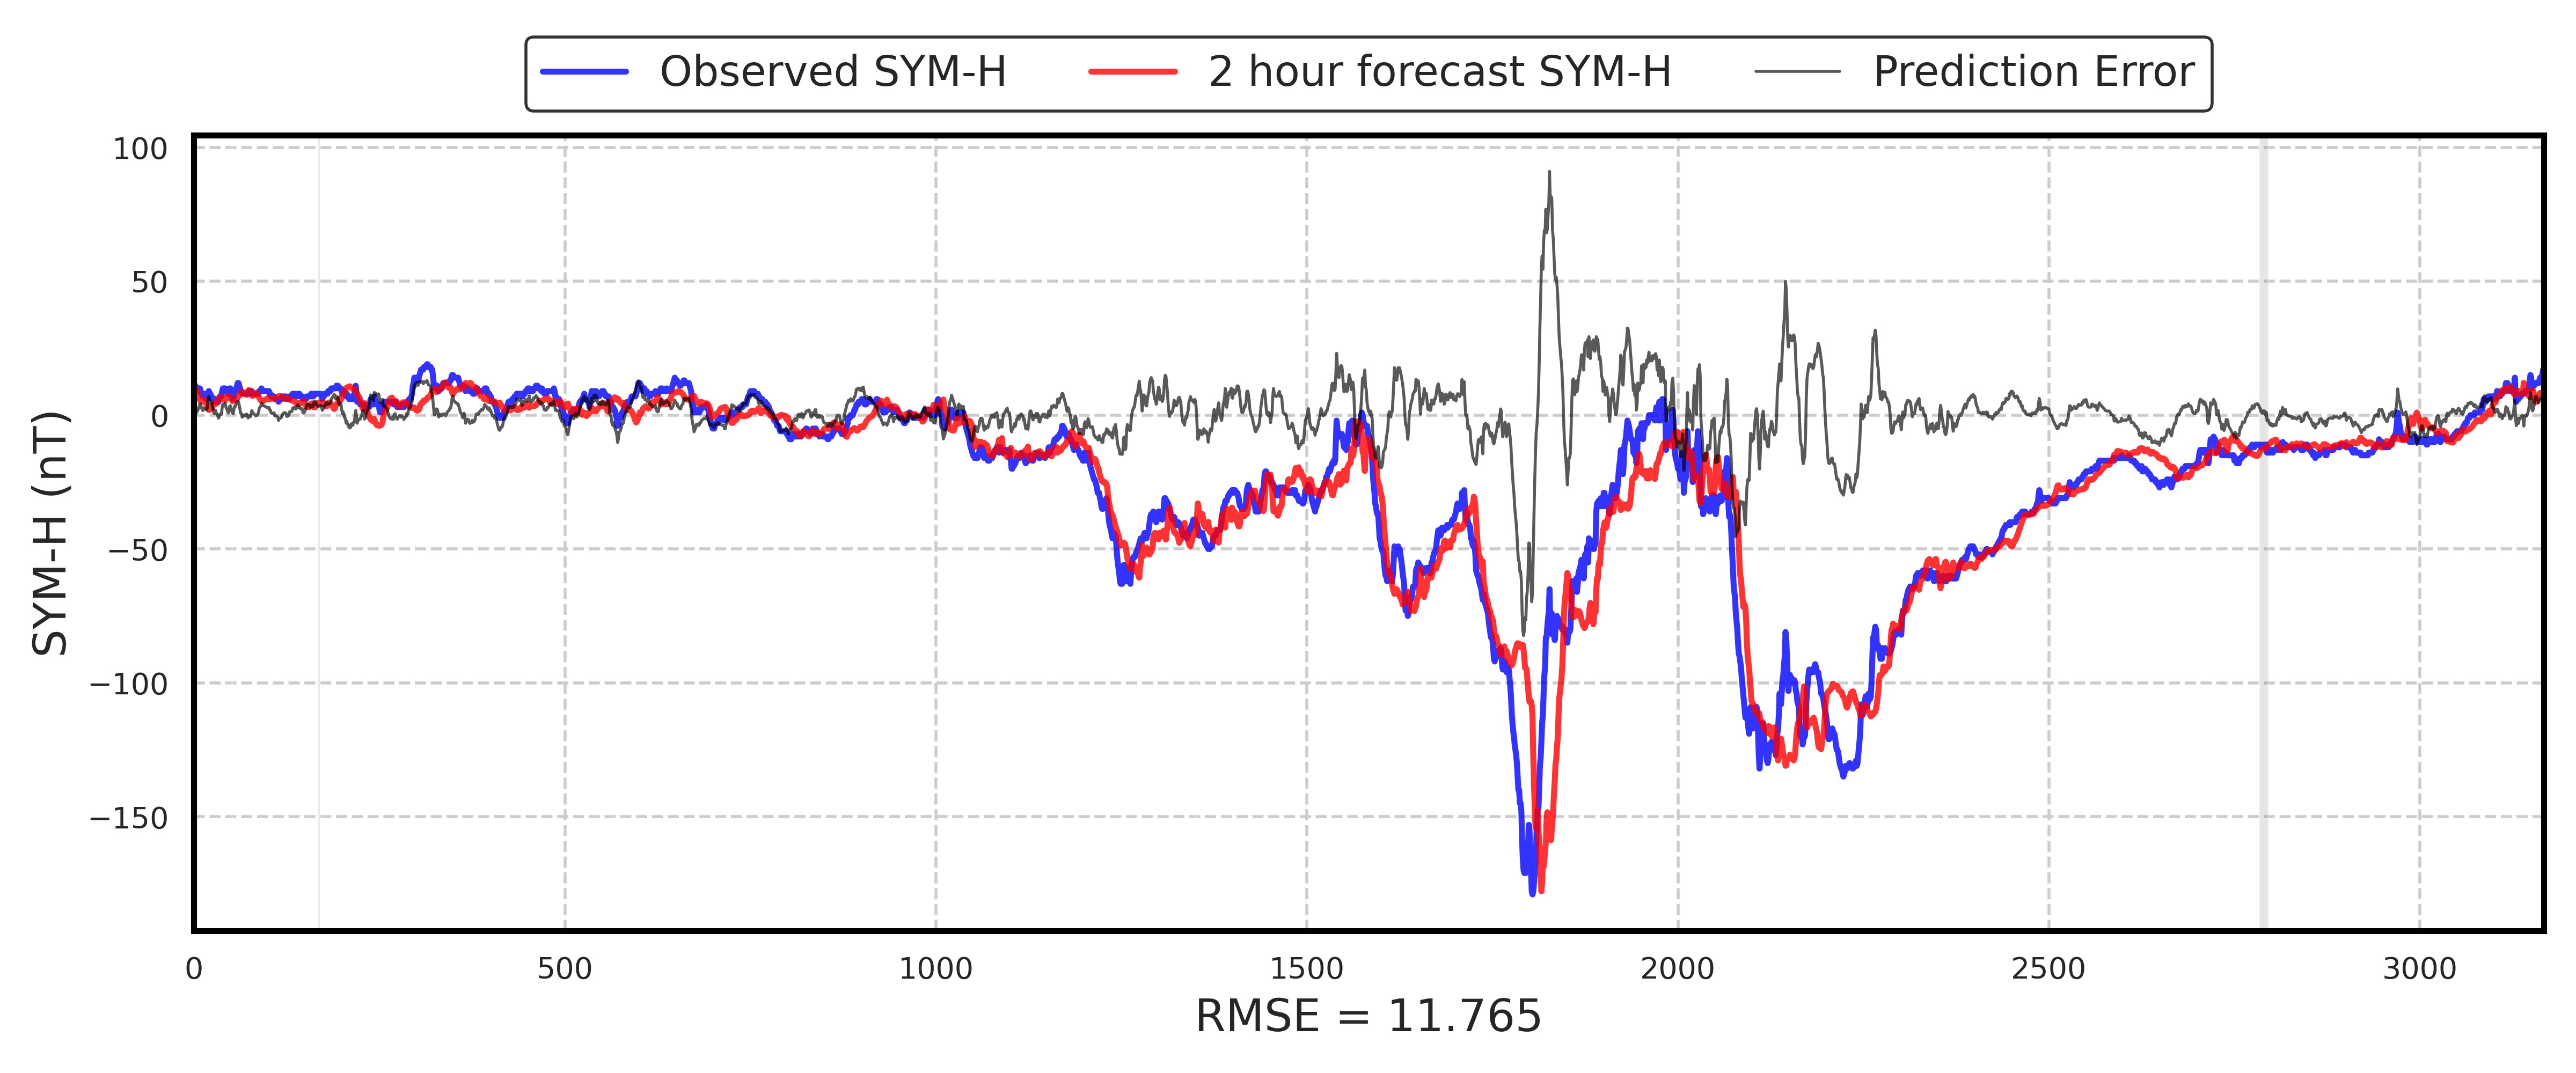
\includegraphics[width=0.49\linewidth]{paper_plots_shade/2h_swics/2h_swics_storm_27.png}
\\
\shortstack{1h forecast using SWICS\\ in laboratory conditions} & \shortstack{2h forecast using SWICS\\ in laboratory conditions}
\vspace*{12pt}
\\
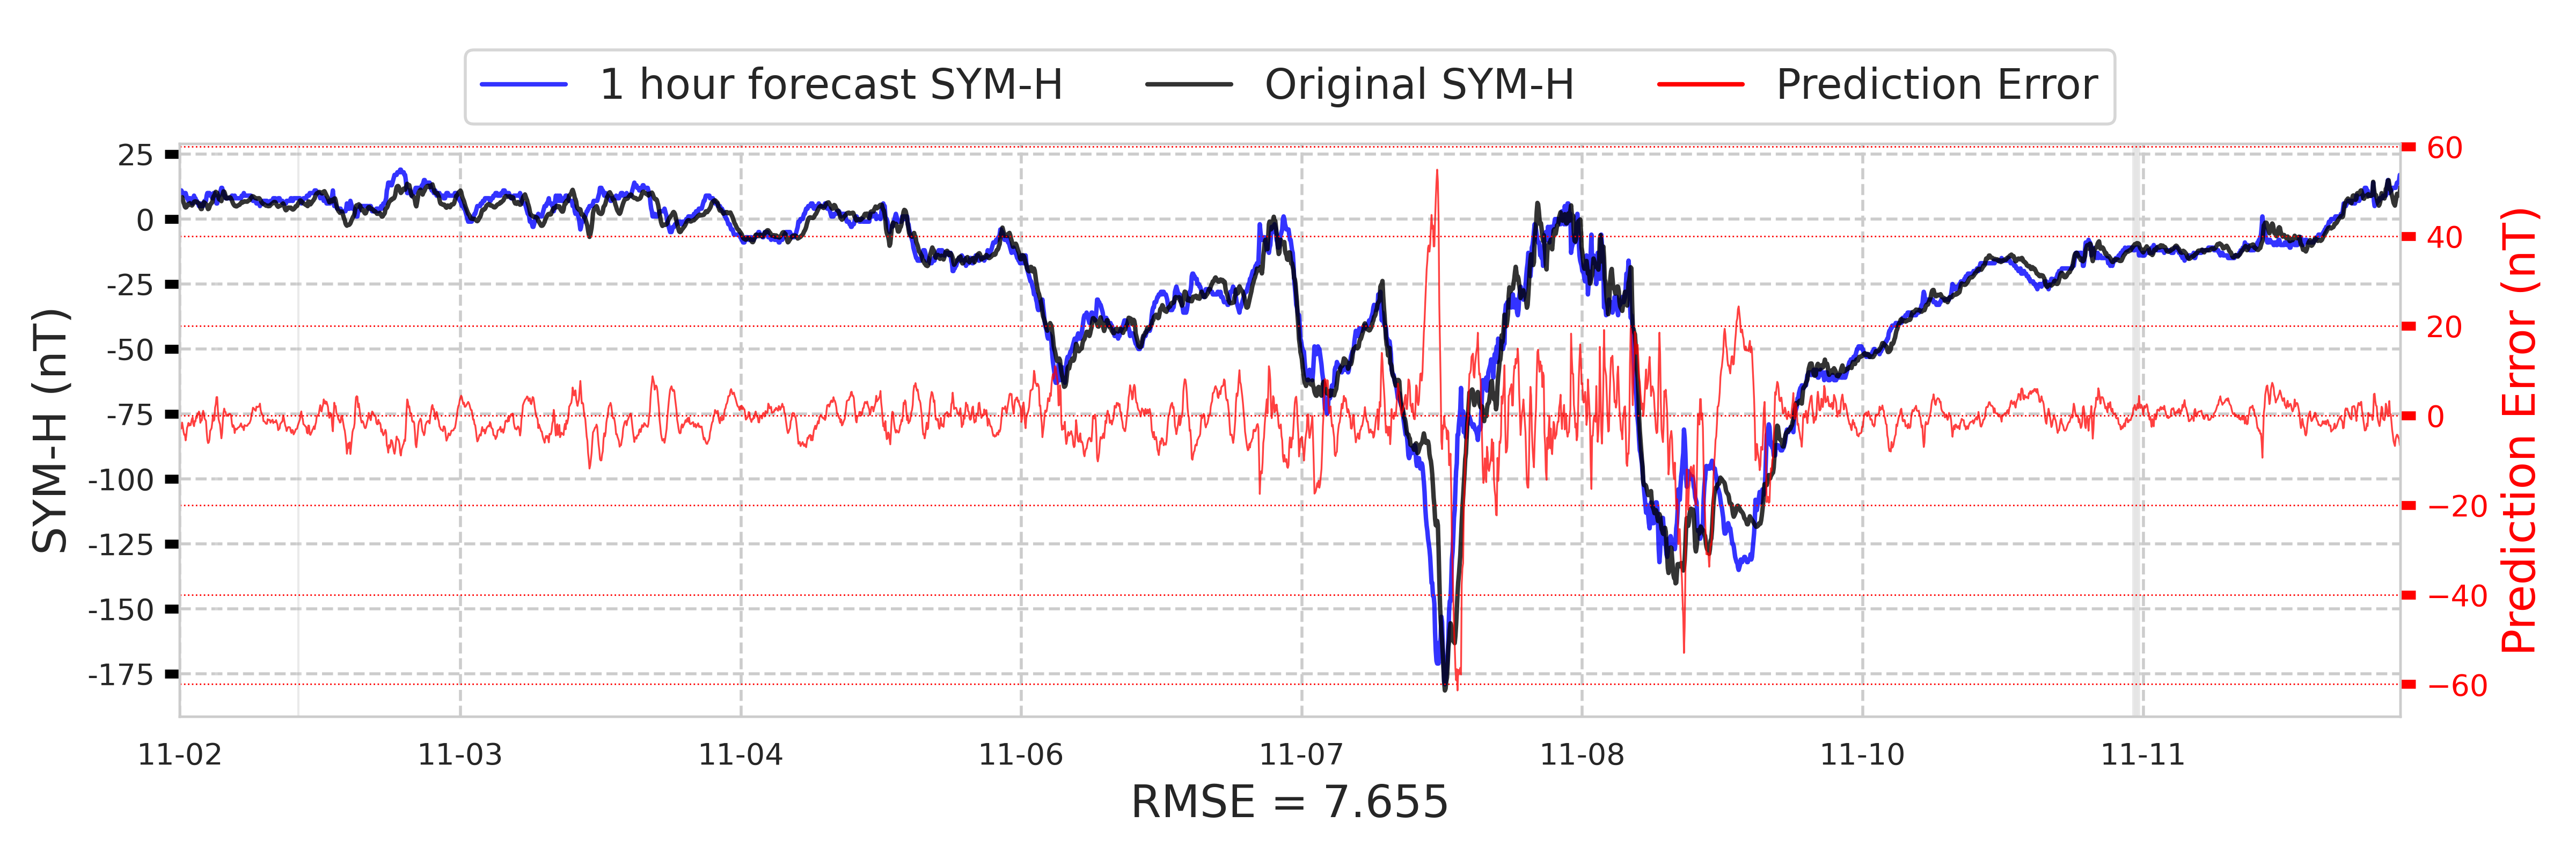
\includegraphics[width=0.49\linewidth]{paper_plots_shade/1h_swics_rt/1h_swics_rt_storm_27.png}
&
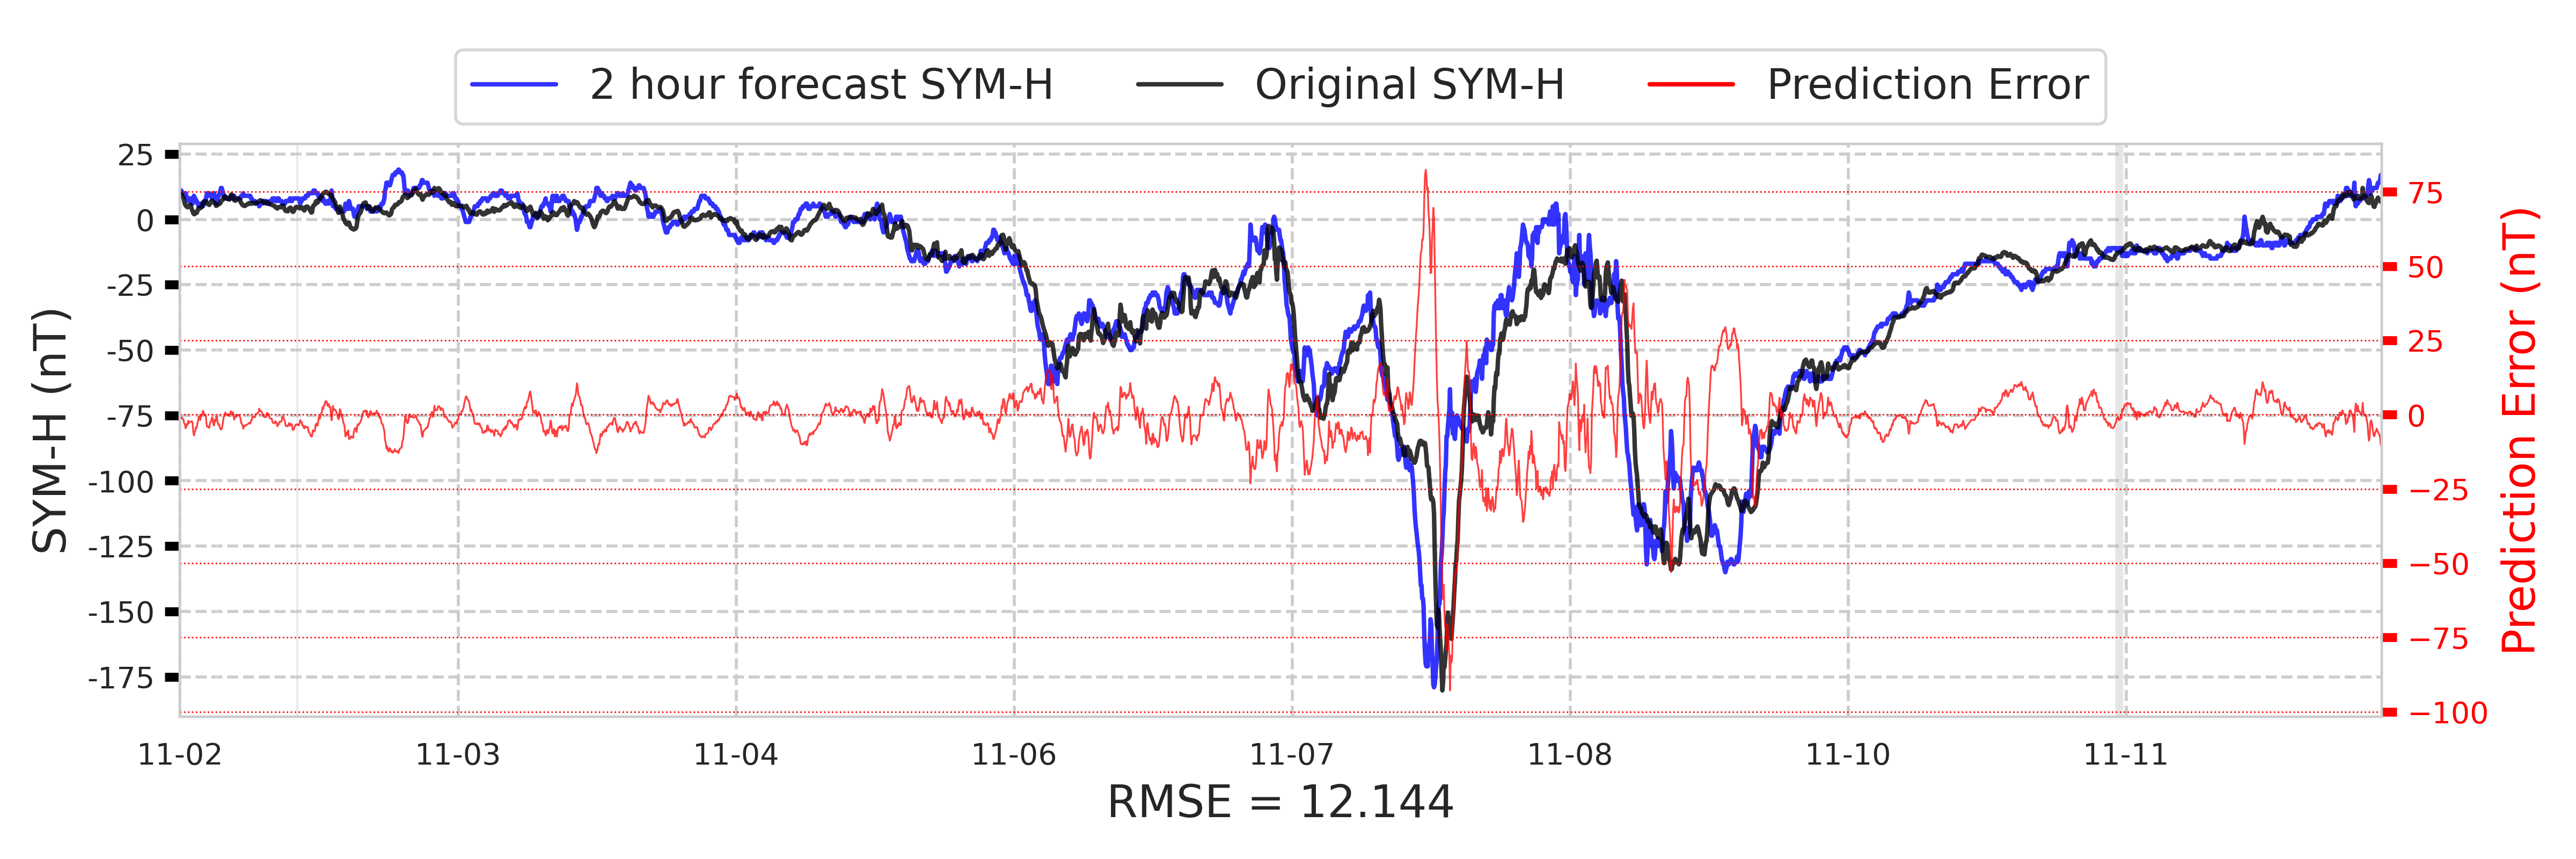
\includegraphics[width=0.49\linewidth]{paper_plots_shade/2h_swics_rt/2h_swics_rt_storm_27.png}
\\
\shortstack{1h operational forecast trained\\ with SWEPAM and SWICS data} & \shortstack{2h operational forecast trained\\ with SWEPAM and SWICS data}
\vspace*{12pt}
\\
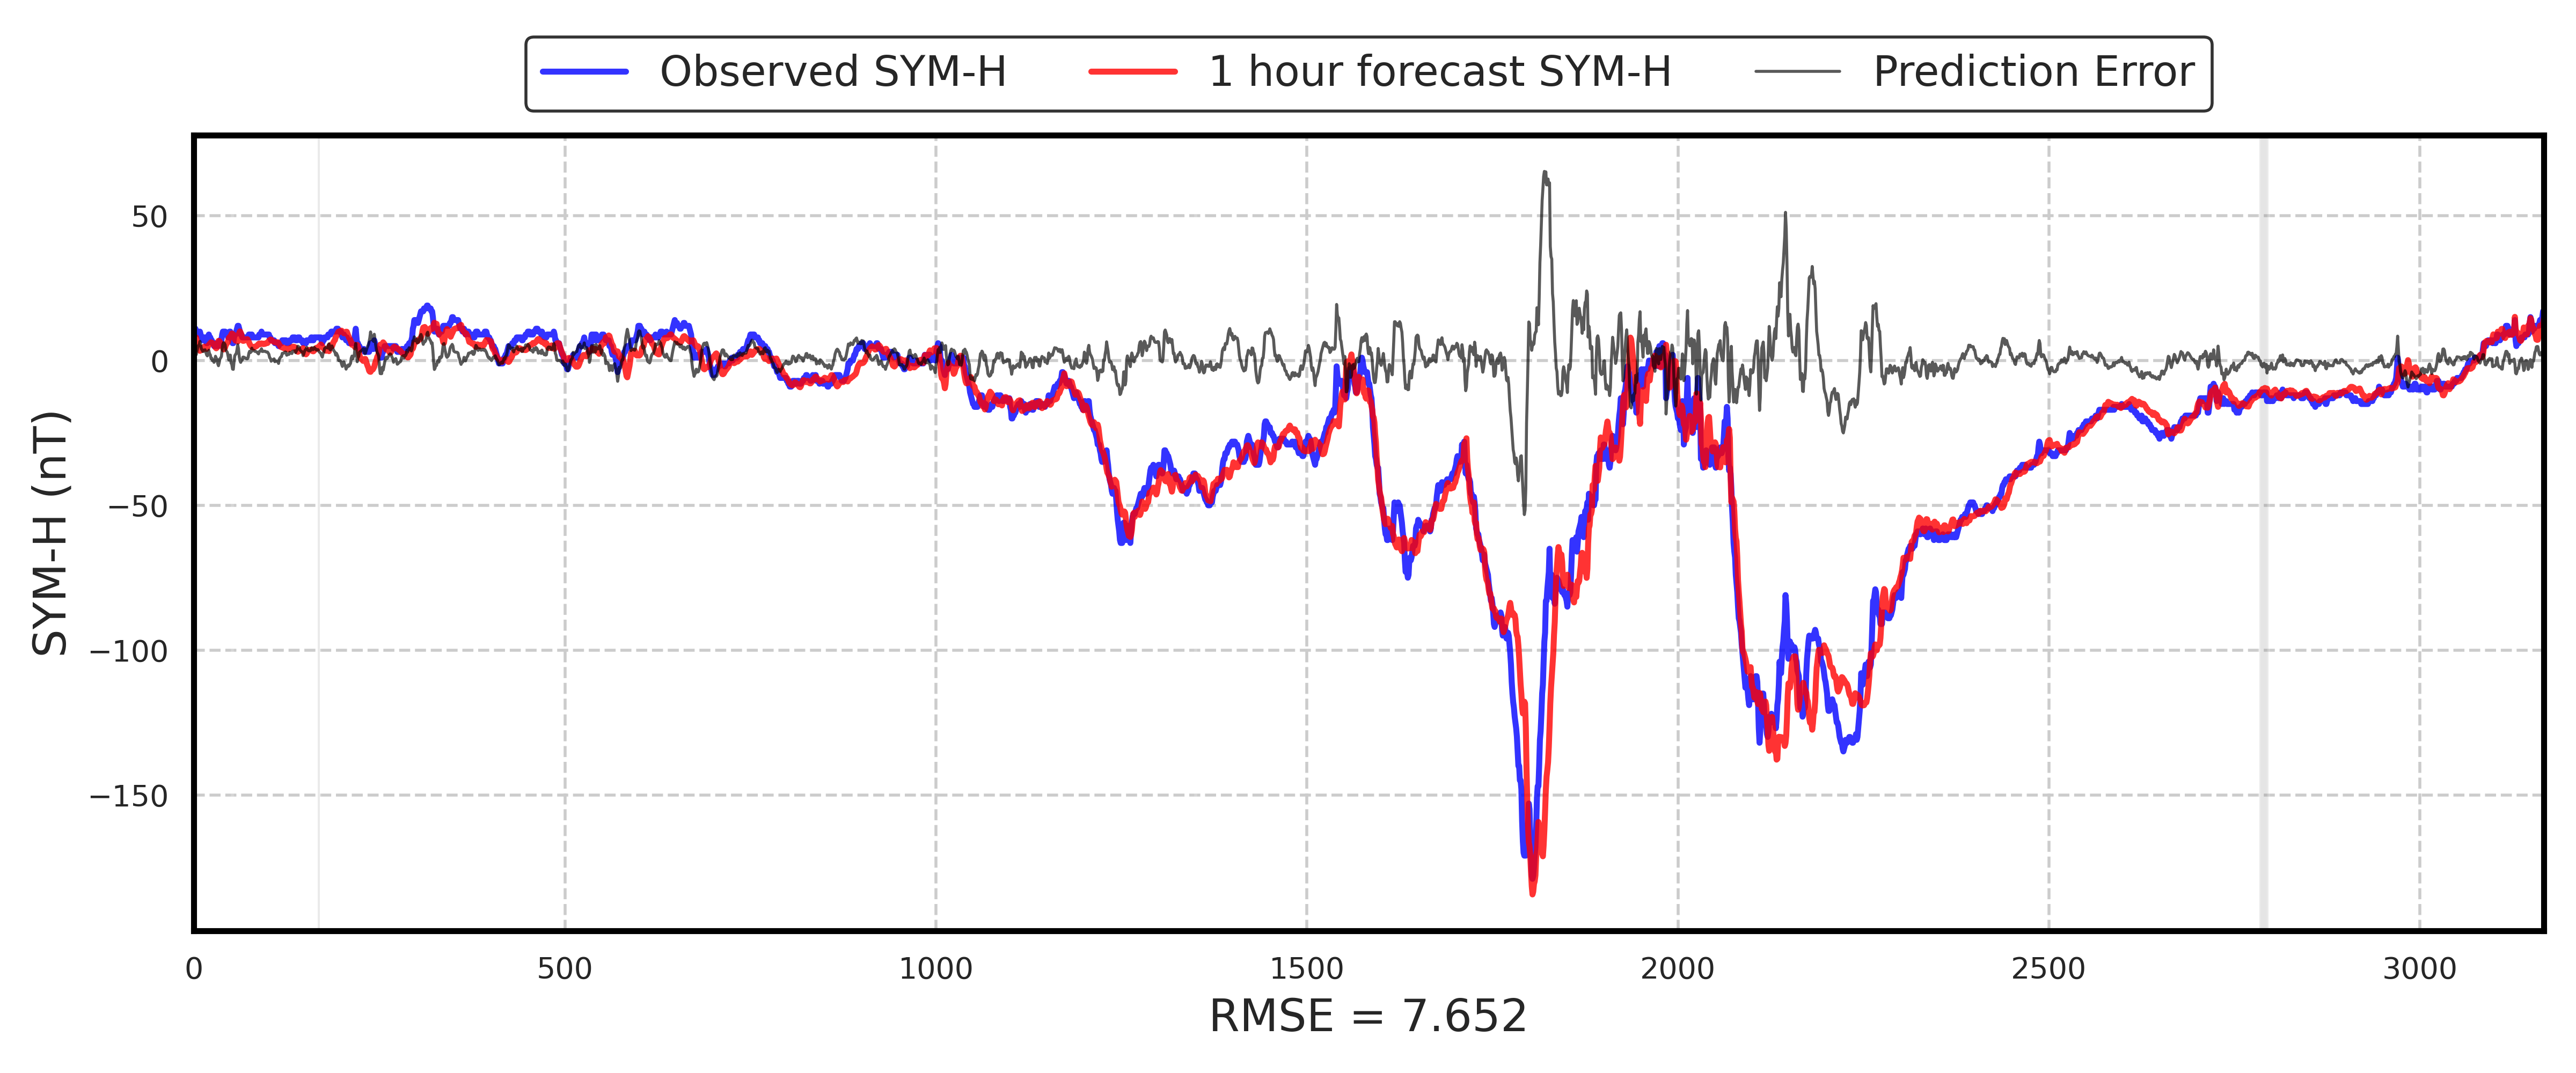
\includegraphics[width=0.49\linewidth]{paper_plots_shade/1h_swepam_rt/1h_swepam_rt_storm_27.png}
&
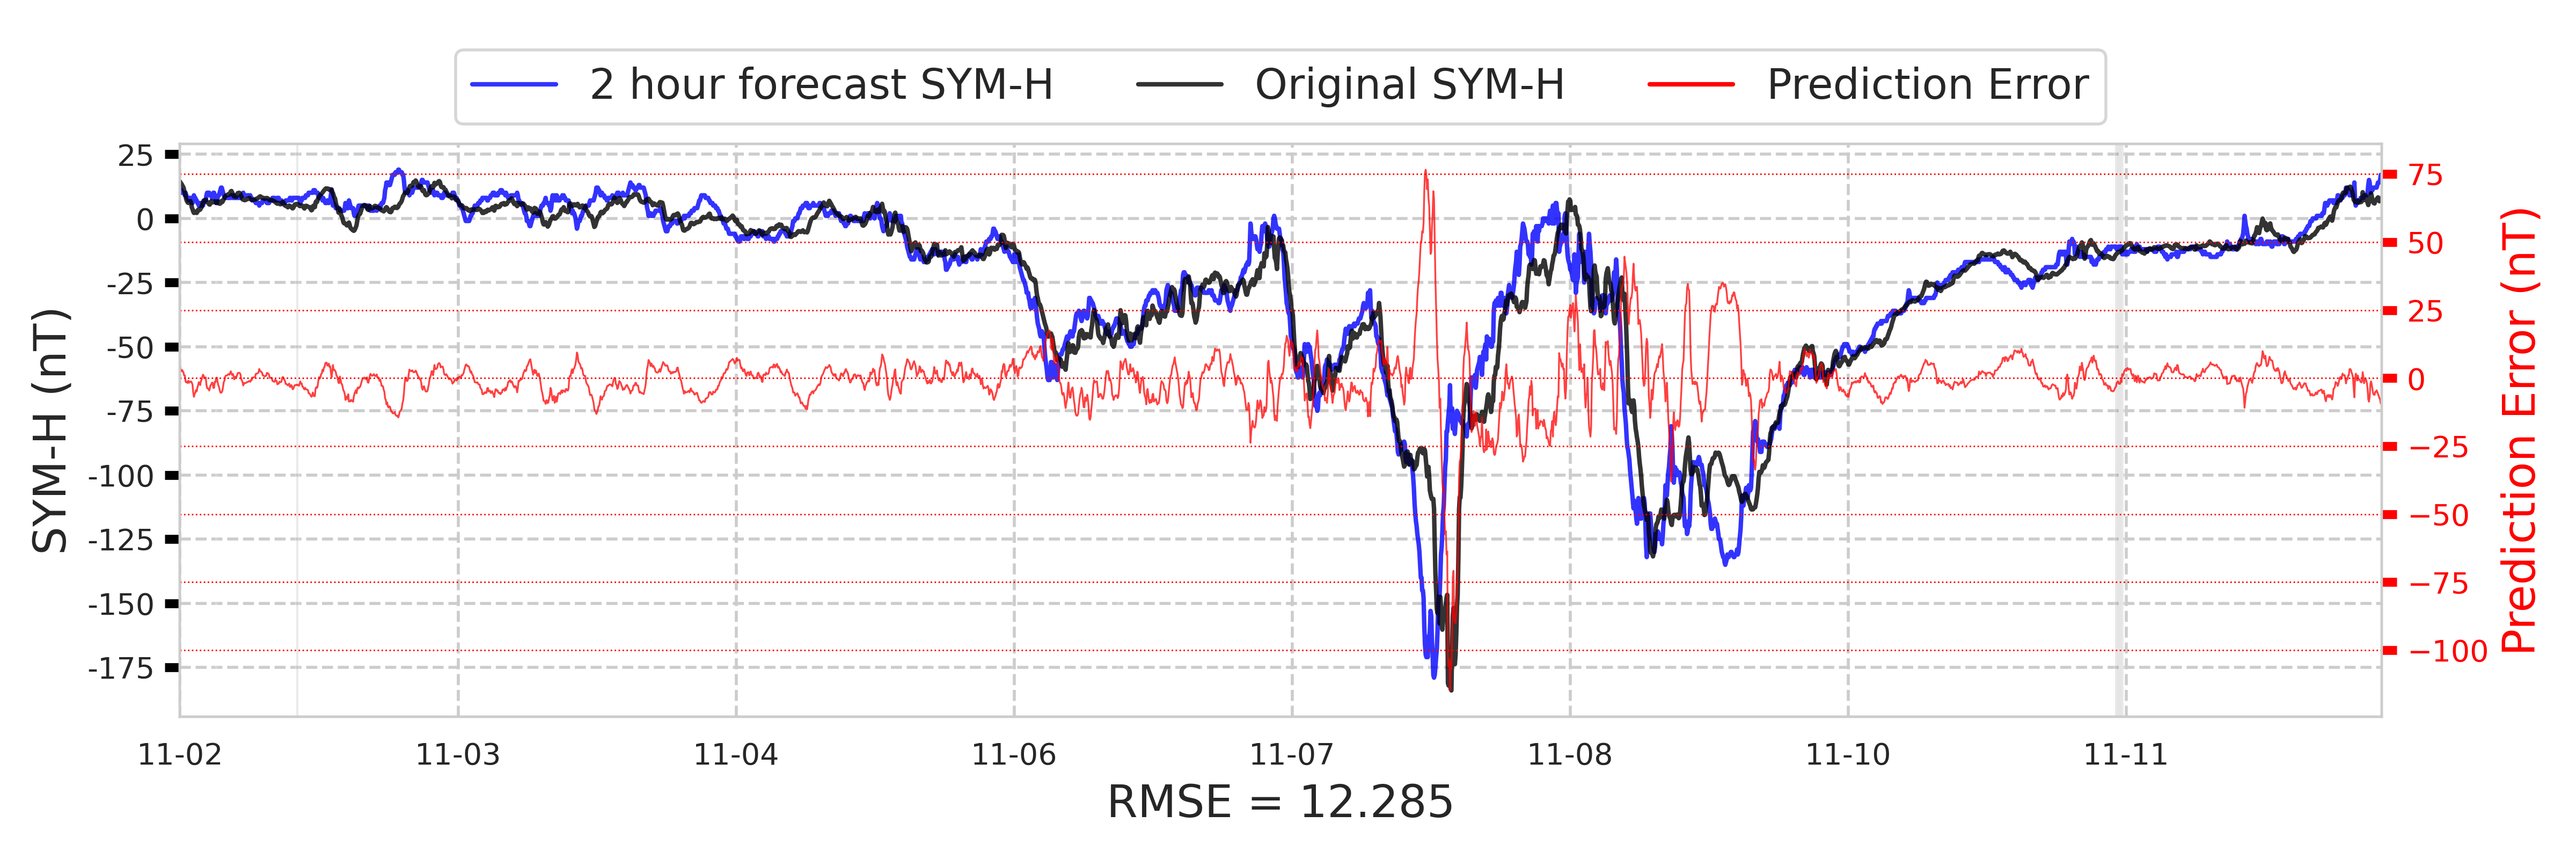
\includegraphics[width=0.49\linewidth]{paper_plots_shade/2h_swepam_rt/2h_swepam_rt_storm_27.png}
\\
\shortstack{1h operational forecast trained\\ with SWEPAM data only} & \shortstack{2h operational forecast trained\\ with SWEPAM data only}
\vspace*{12pt}
\\
\end{tabular}
\caption{Predictions for Storm Number 27 -- November of 1998}
\label{storm-27}
\end{table}



% Figure for storm 28
\begin{table}
\centering
\begin{tabular}{cc}
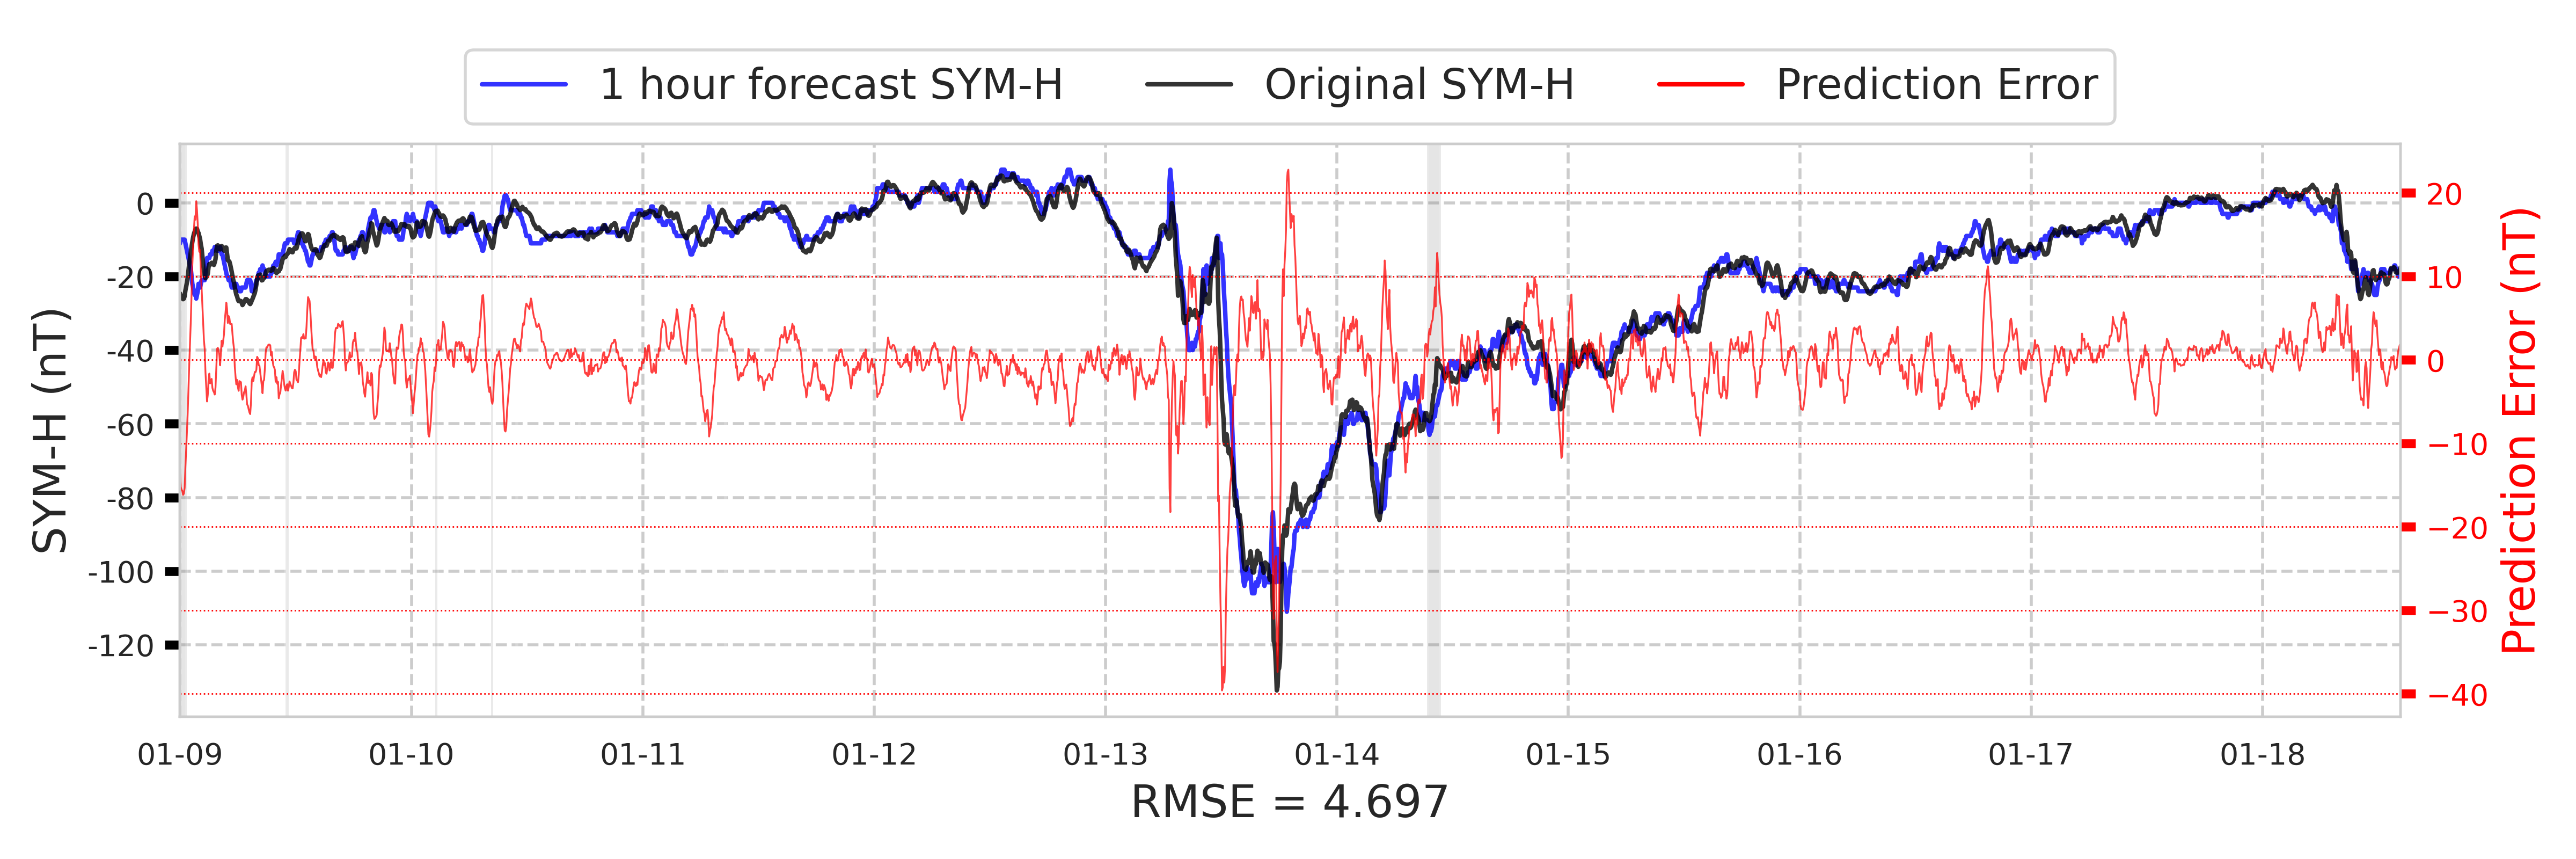
\includegraphics[width=0.49\linewidth]{paper_plots_shade/1h_swics/1h_swics_storm_28.png}
&
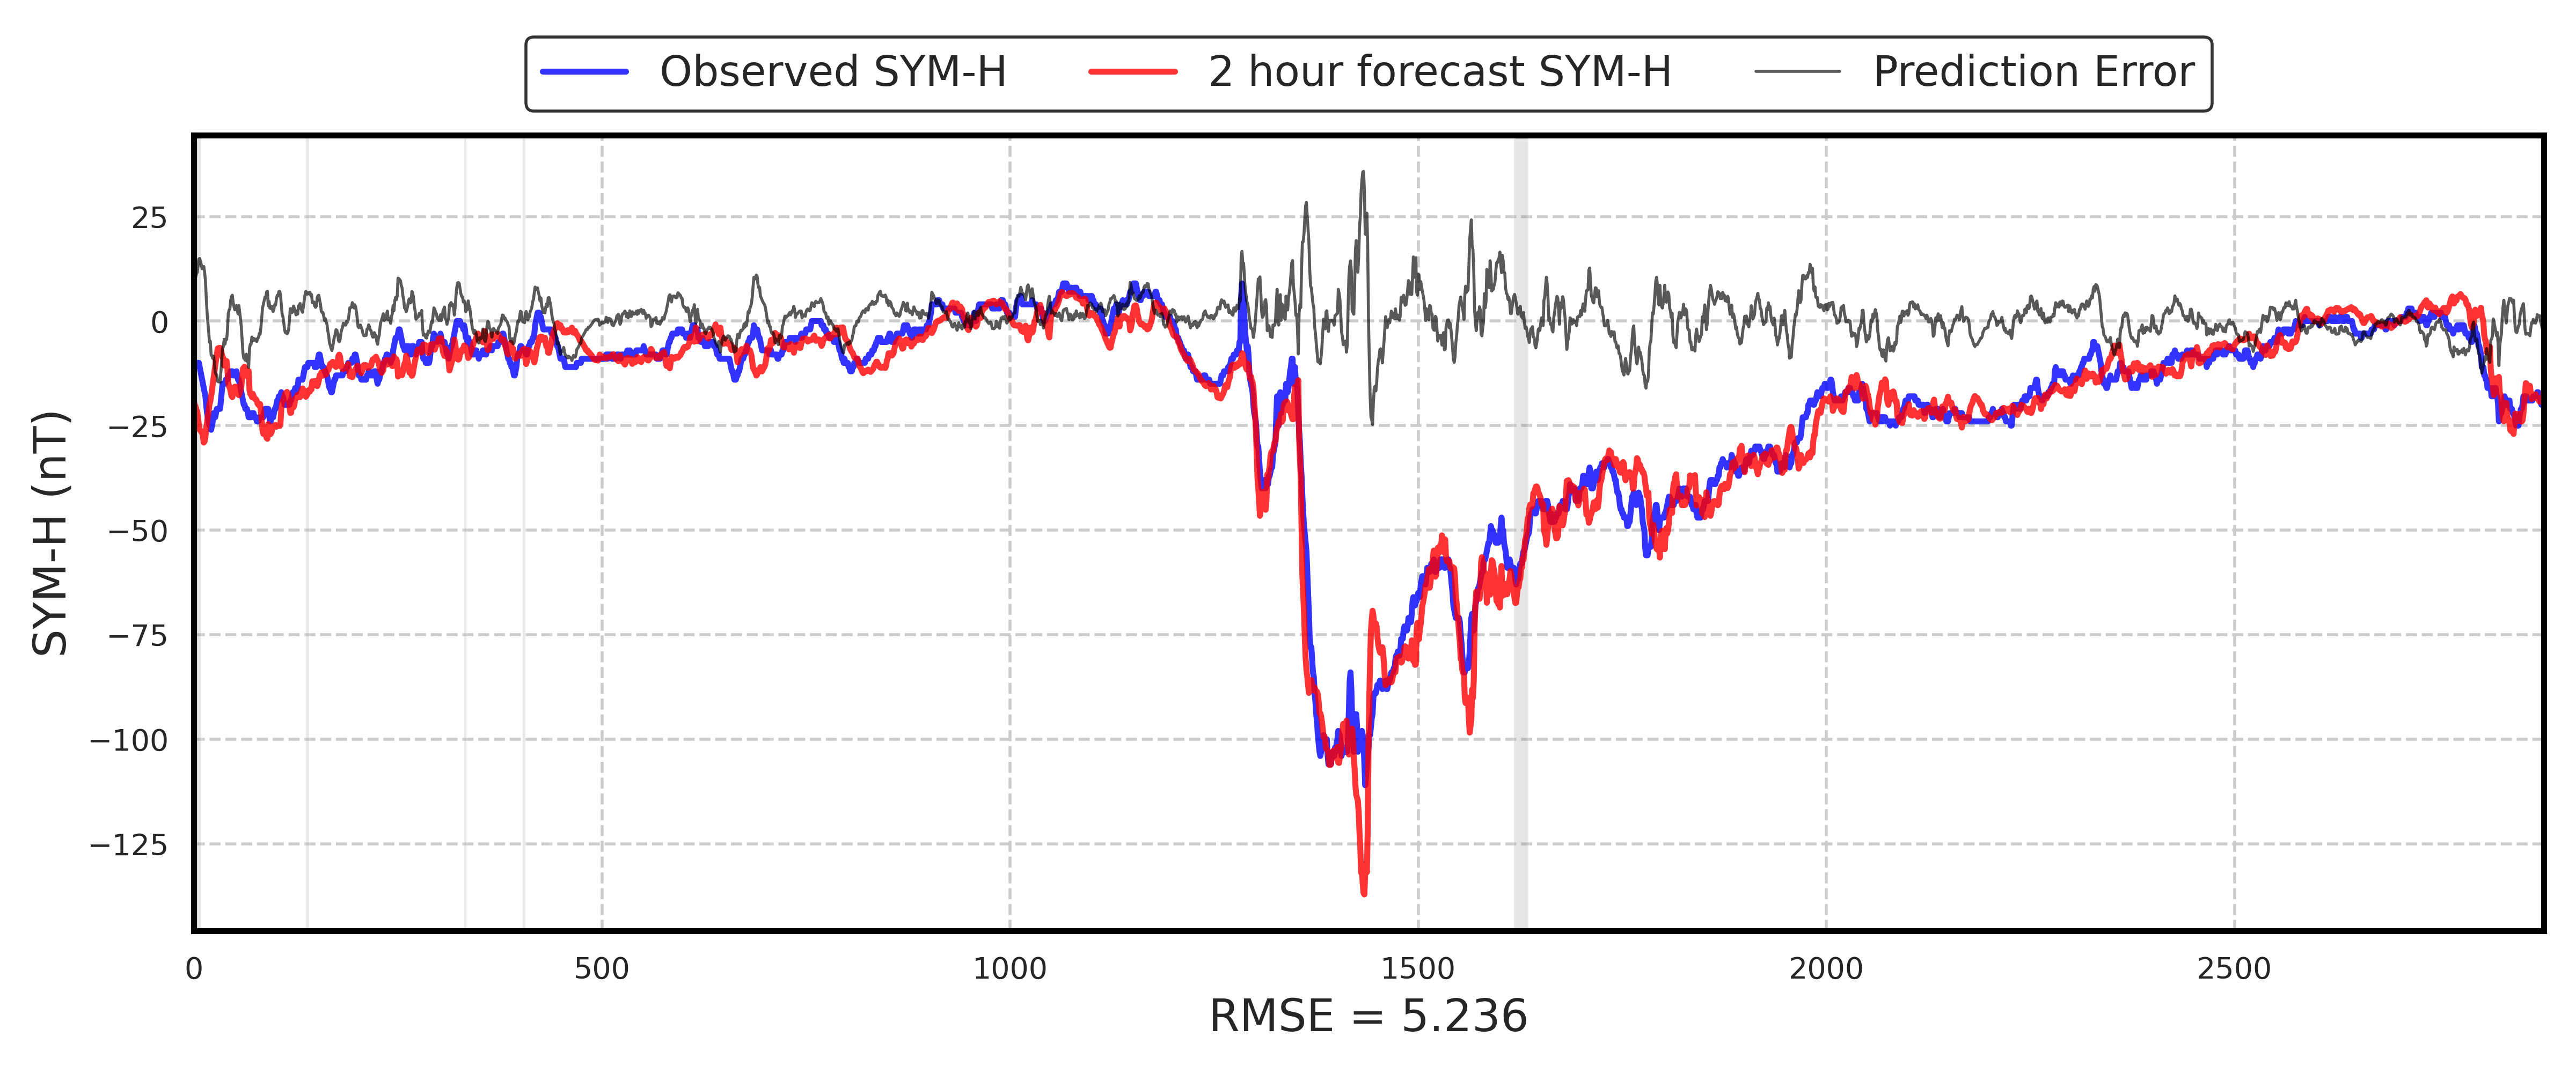
\includegraphics[width=0.49\linewidth]{paper_plots_shade/2h_swics/2h_swics_storm_28.png}
\\
\shortstack{1h forecast using SWICS\\ in laboratory conditions} & \shortstack{2h forecast using SWICS\\ in laboratory conditions}
\vspace*{12pt}
\\
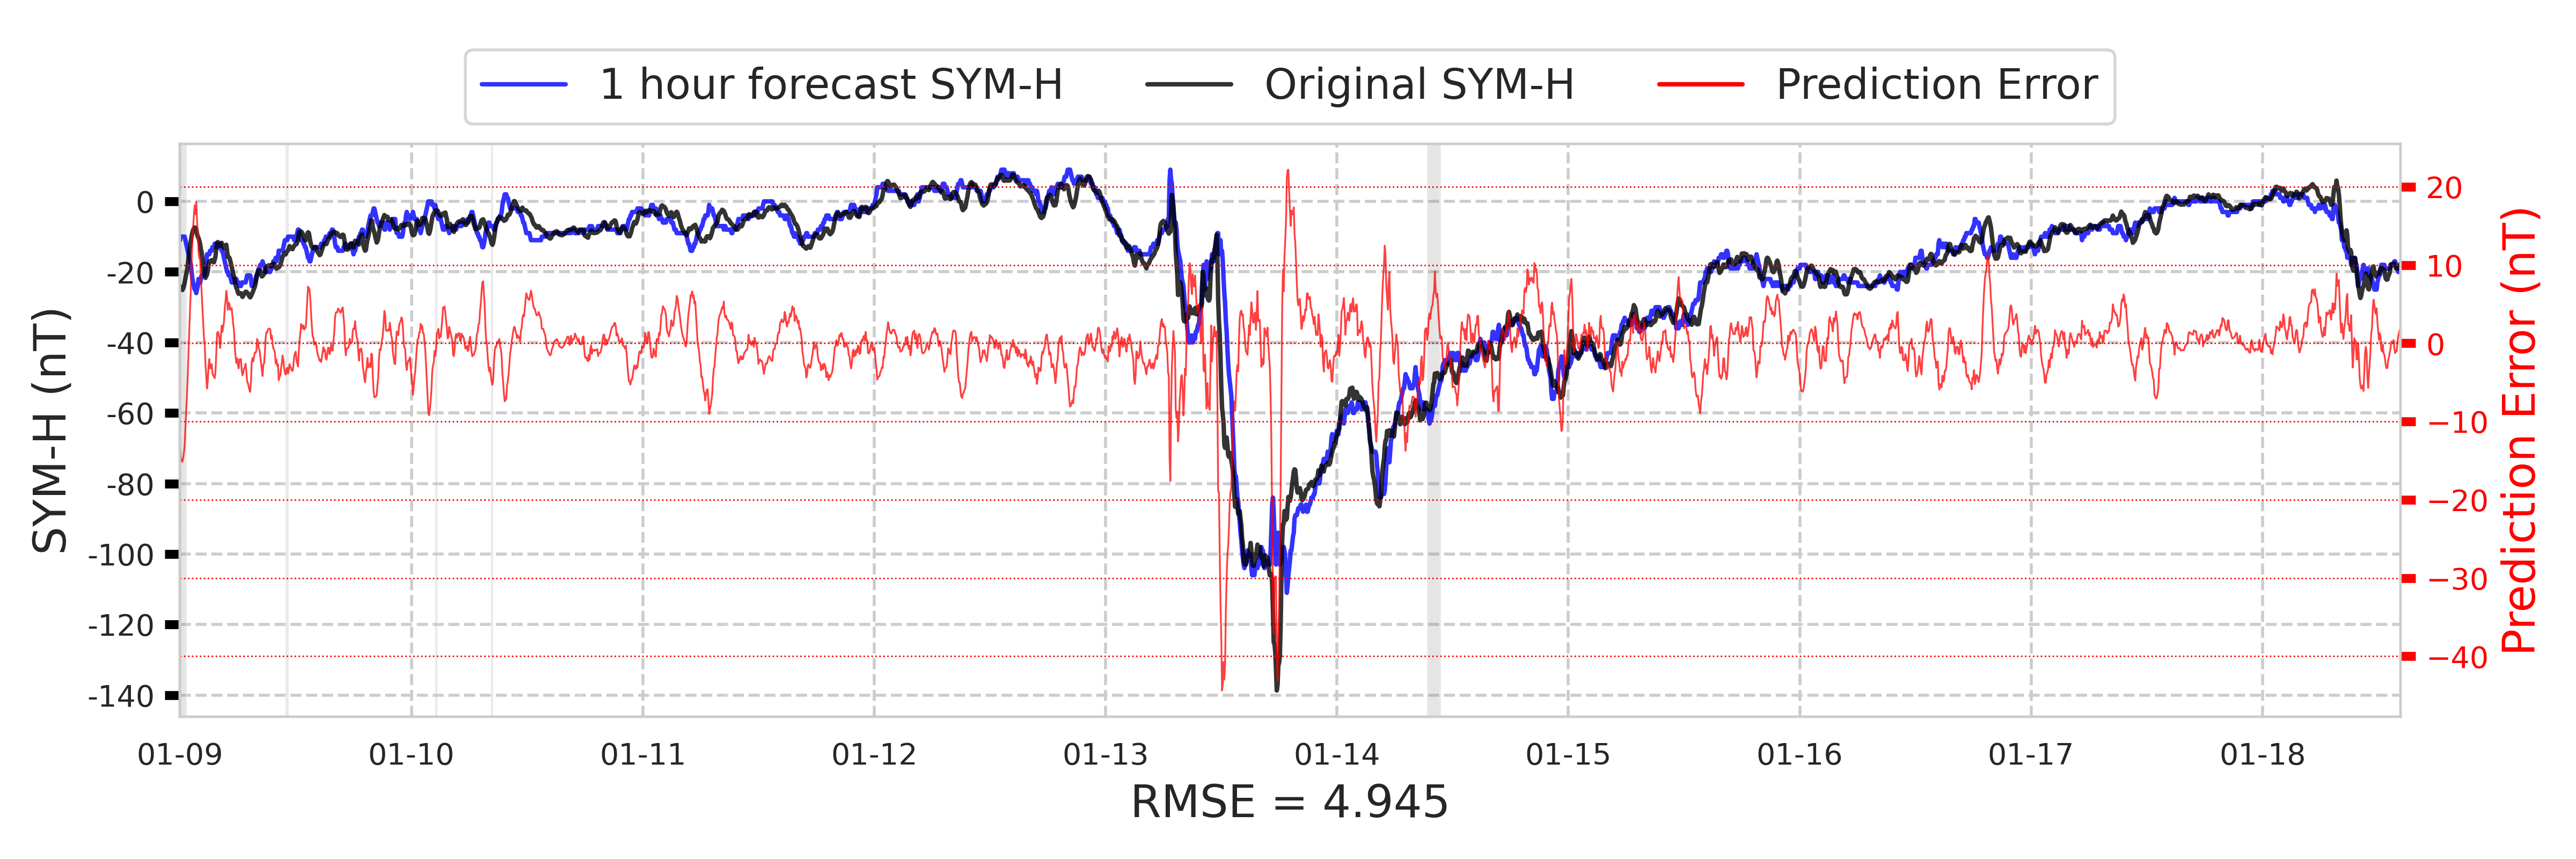
\includegraphics[width=0.49\linewidth]{paper_plots_shade/1h_swics_rt/1h_swics_rt_storm_28.png}
&
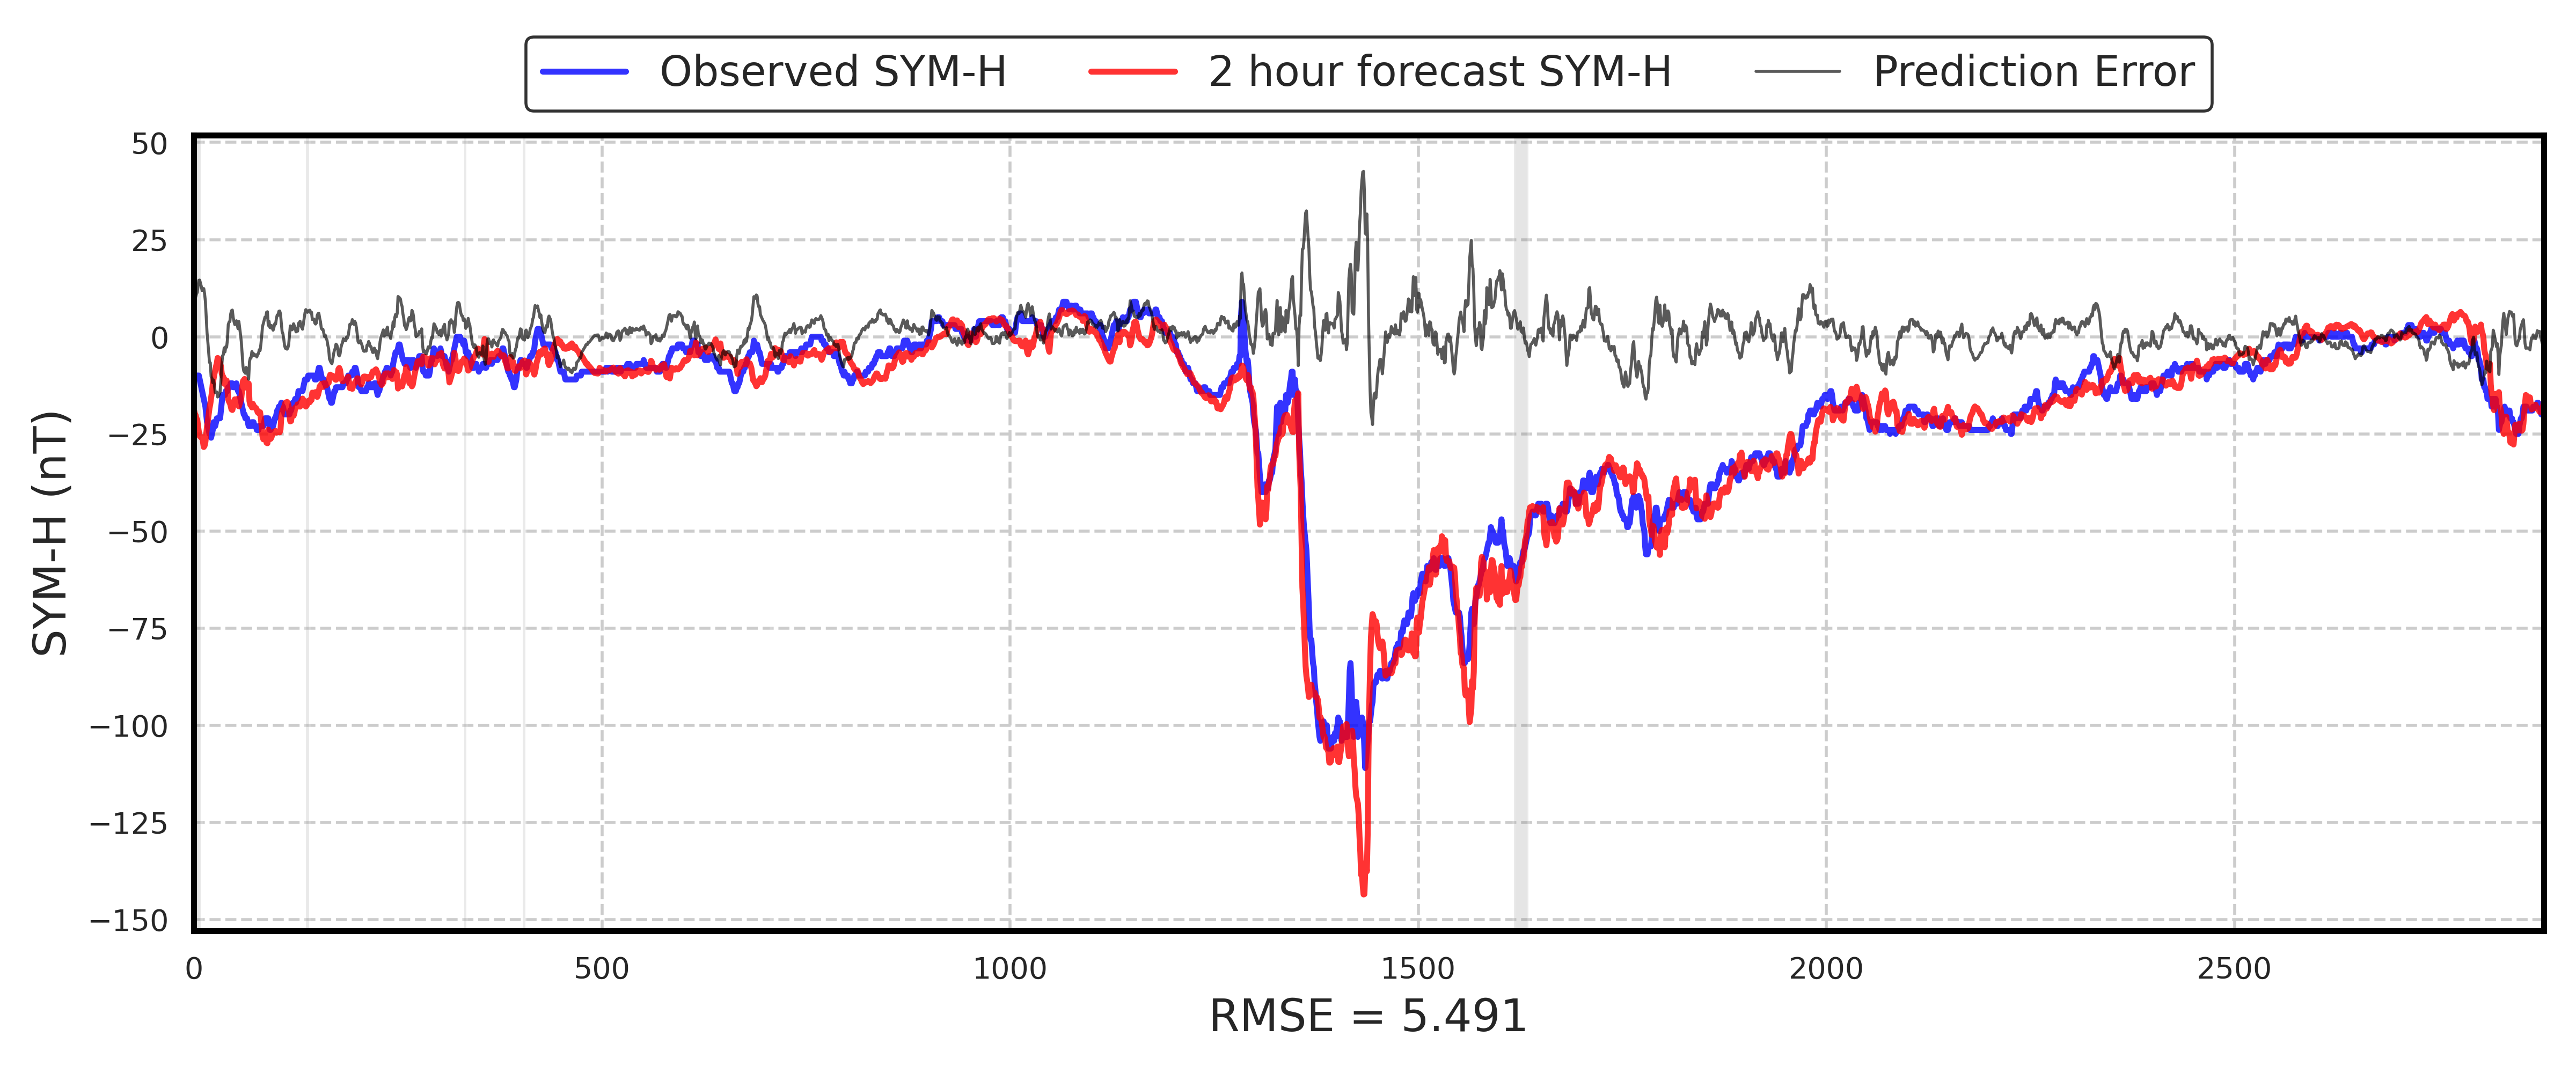
\includegraphics[width=0.49\linewidth]{paper_plots_shade/2h_swics_rt/2h_swics_rt_storm_28.png}
\\
\shortstack{1h operational forecast trained\\ with SWEPAM and SWICS data} & \shortstack{2h operational forecast trained\\ with SWEPAM and SWICS data}
\vspace*{12pt}
\\
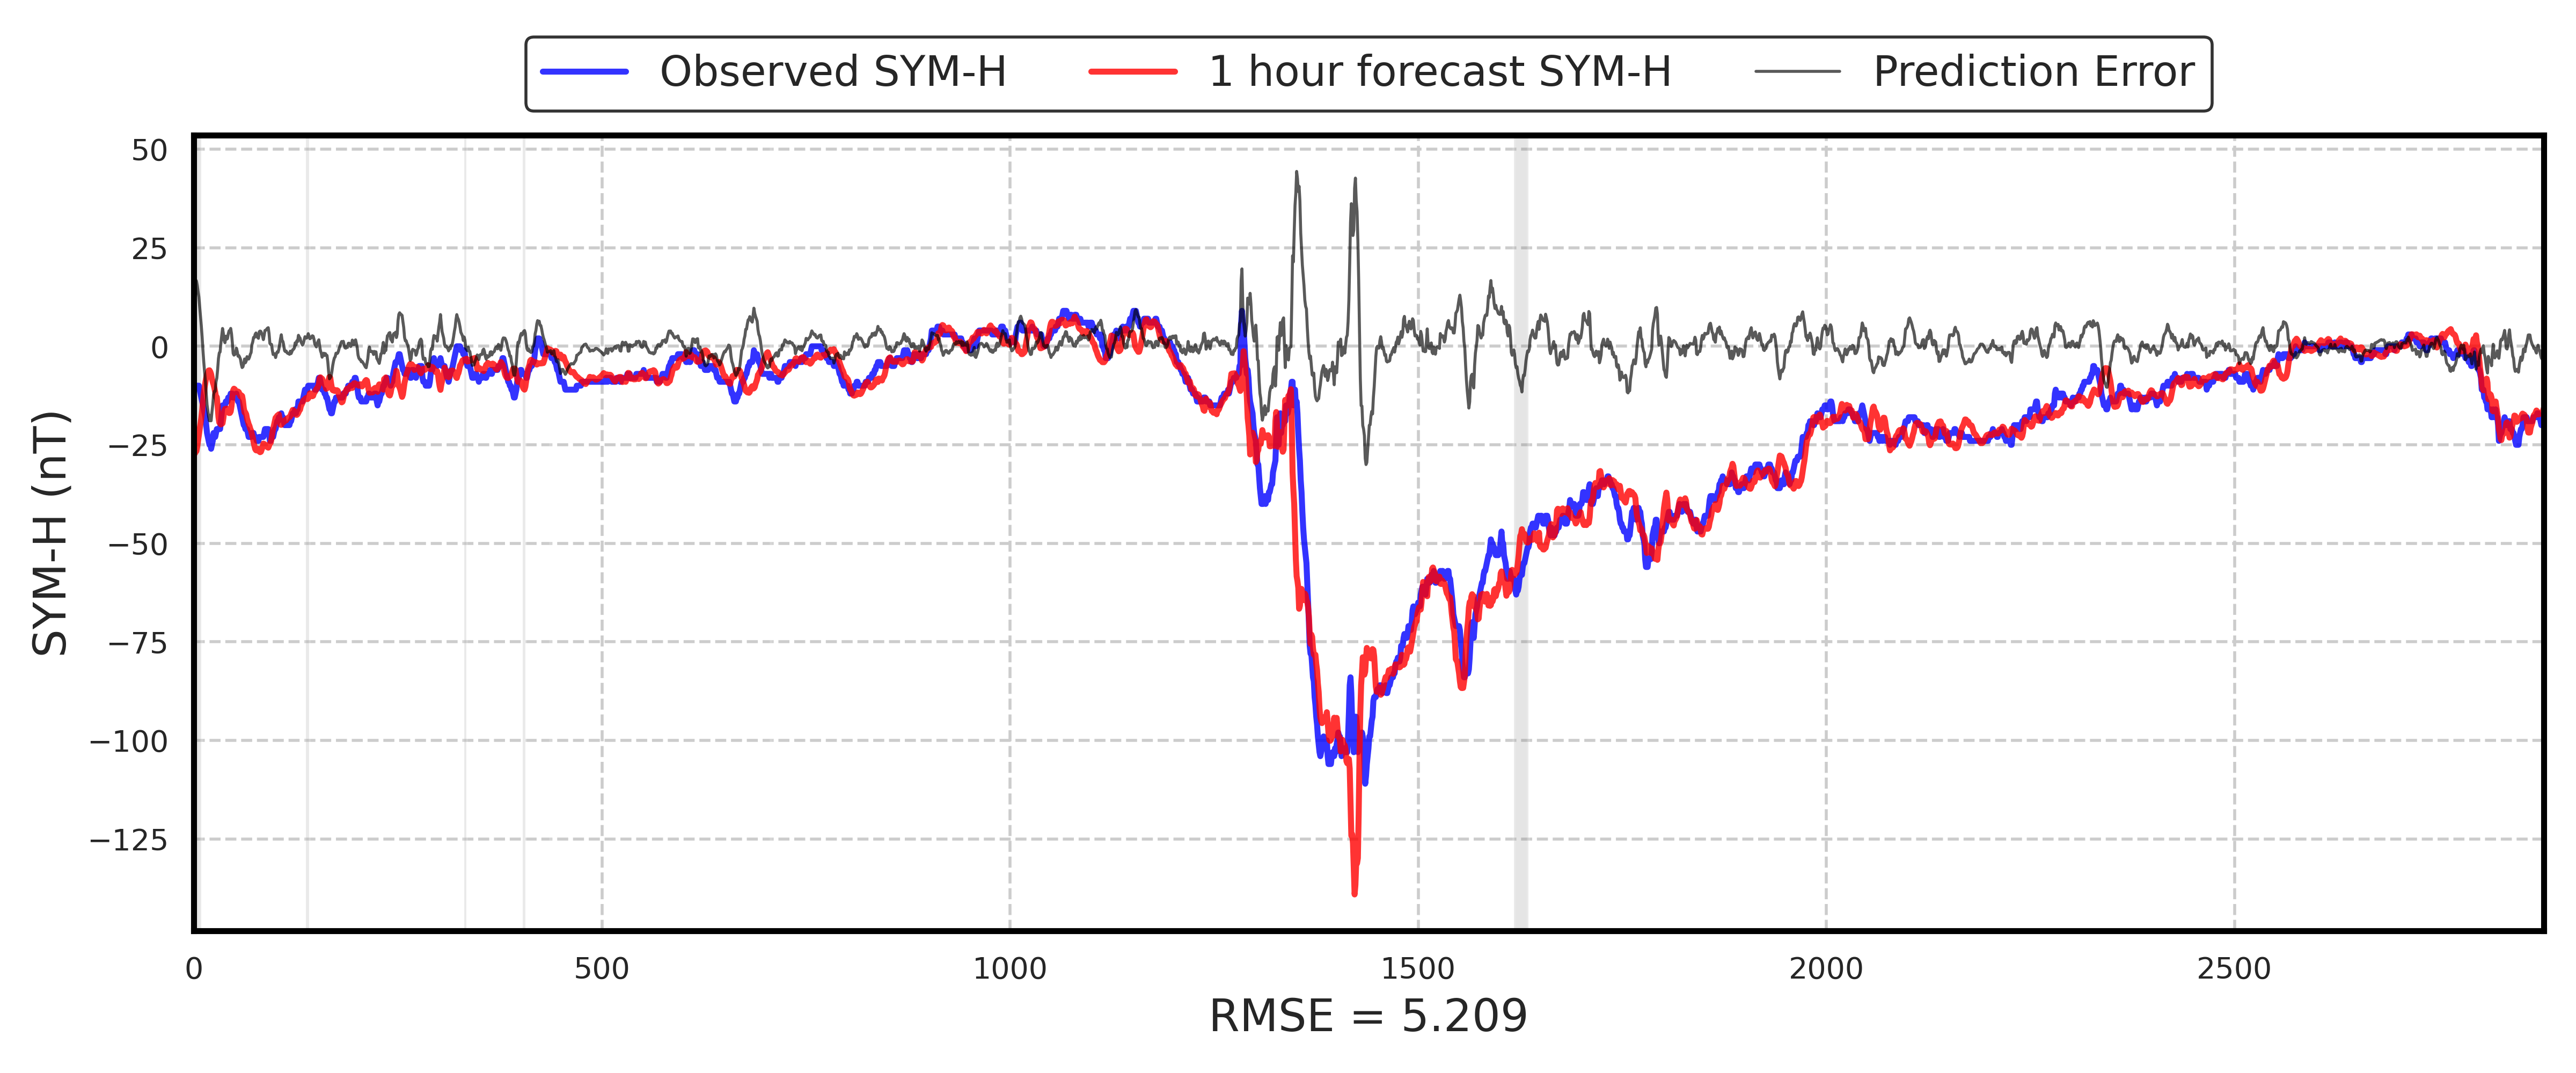
\includegraphics[width=0.49\linewidth]{paper_plots_shade/1h_swepam_rt/1h_swepam_rt_storm_28.png}
&
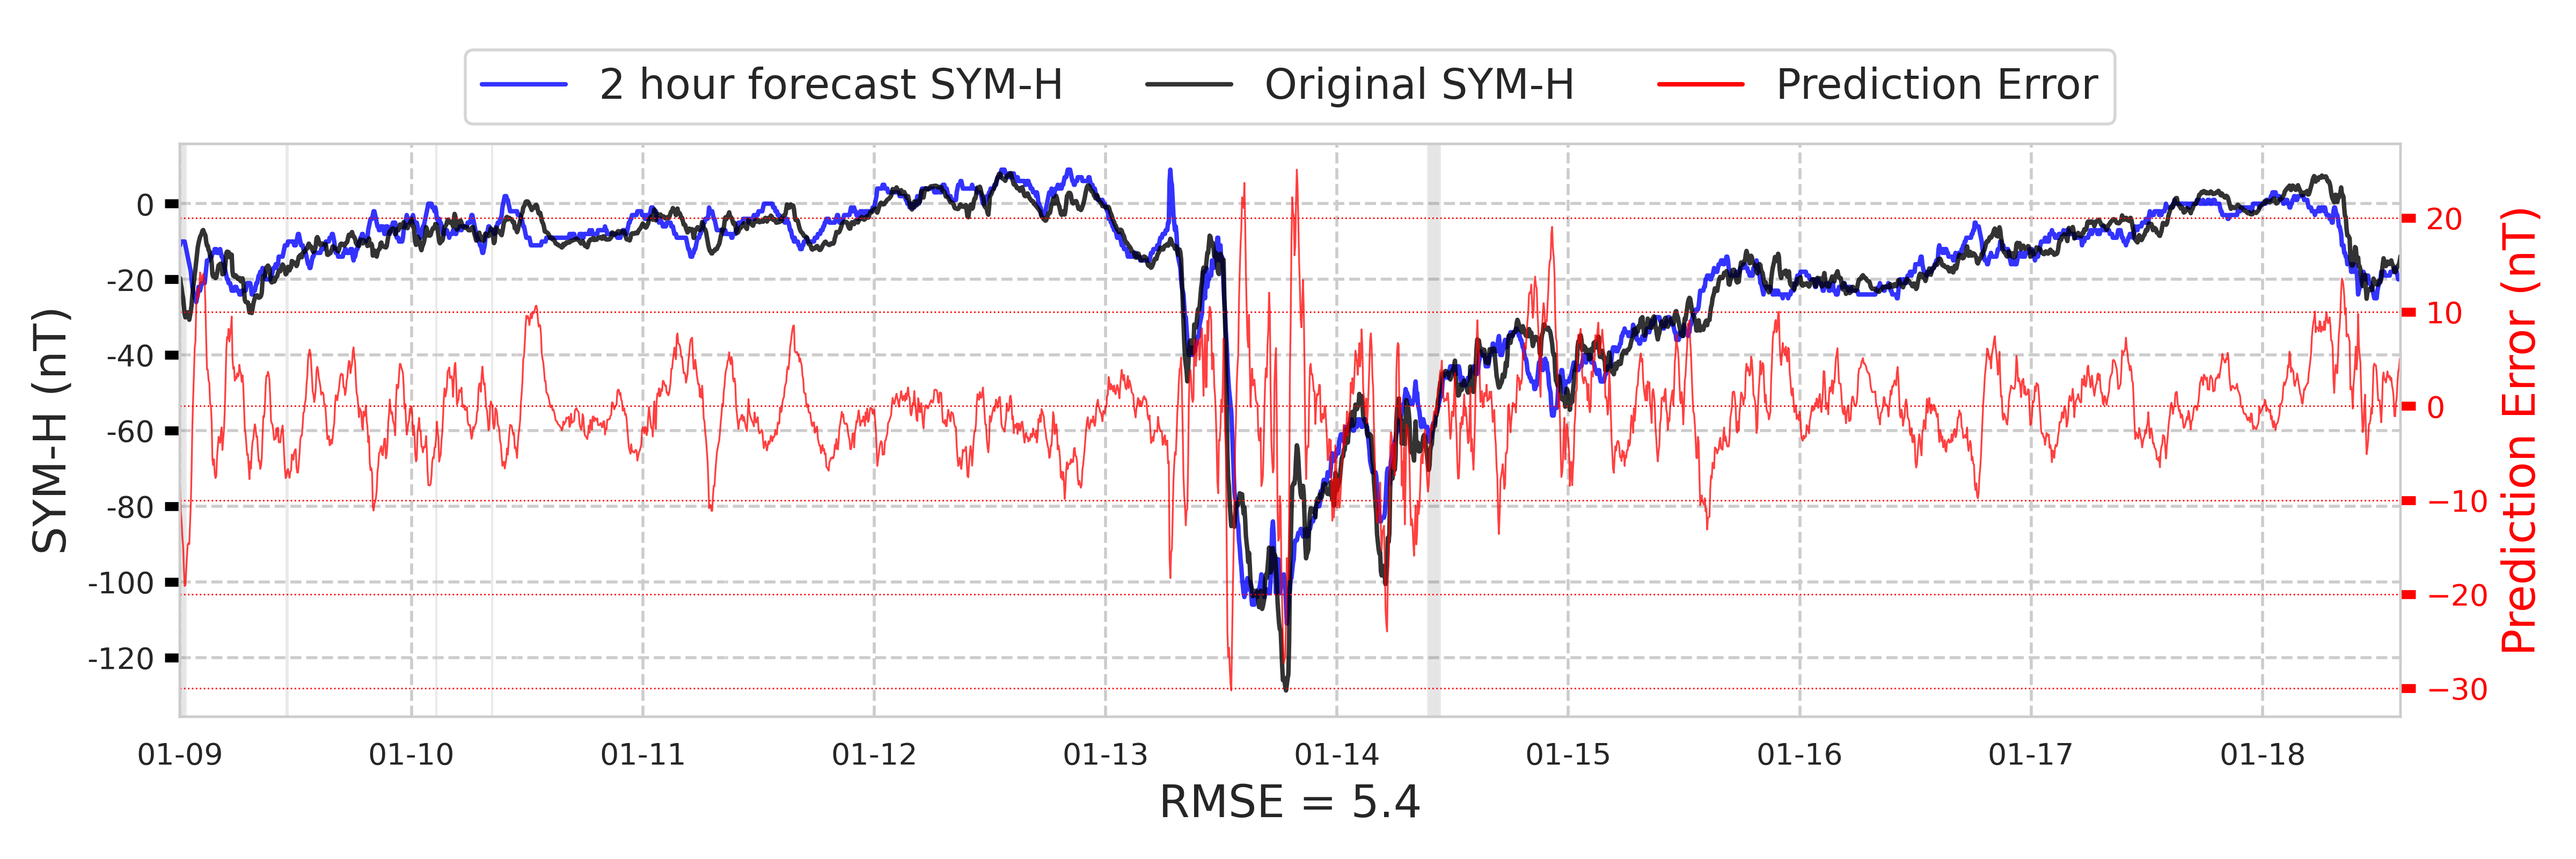
\includegraphics[width=0.49\linewidth]{paper_plots_shade/2h_swepam_rt/2h_swepam_rt_storm_28.png}
\\
\shortstack{1h operational forecast trained\\ with SWEPAM data only} & \shortstack{2h operational forecast trained\\ with SWEPAM data only}
\vspace*{12pt}
\\
\end{tabular}
\caption{Predictions for Storm Number 28 -- January of 1999}
\label{storm-28}
\end{table}



% Figure for storm 29
\begin{table}
\centering
\begin{tabular}{cc}
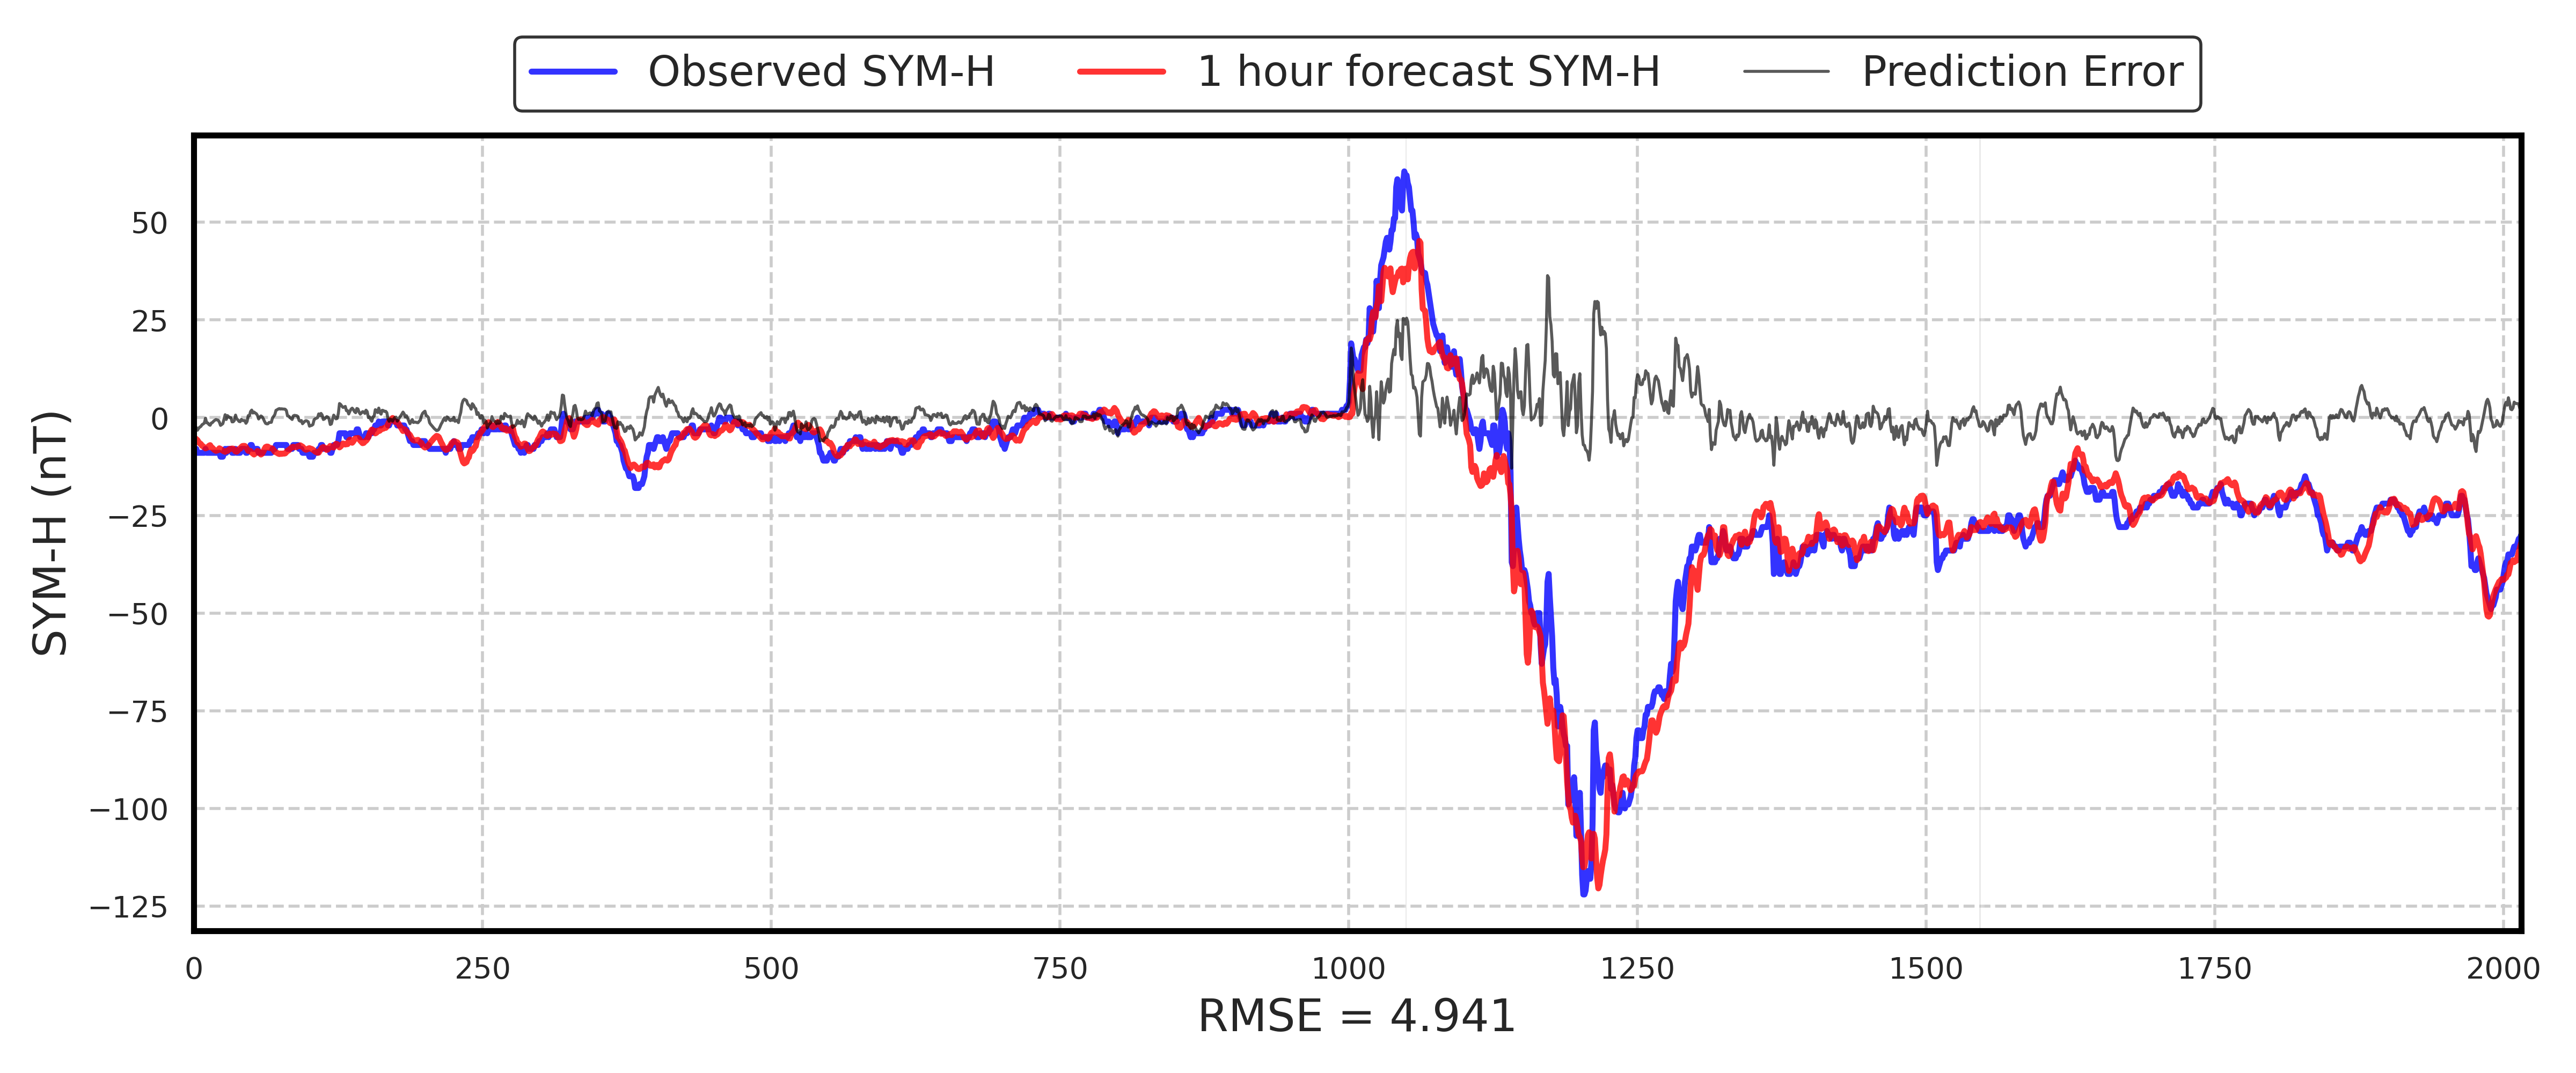
\includegraphics[width=0.49\linewidth]{paper_plots_shade/1h_swics/1h_swics_storm_29.png}
&
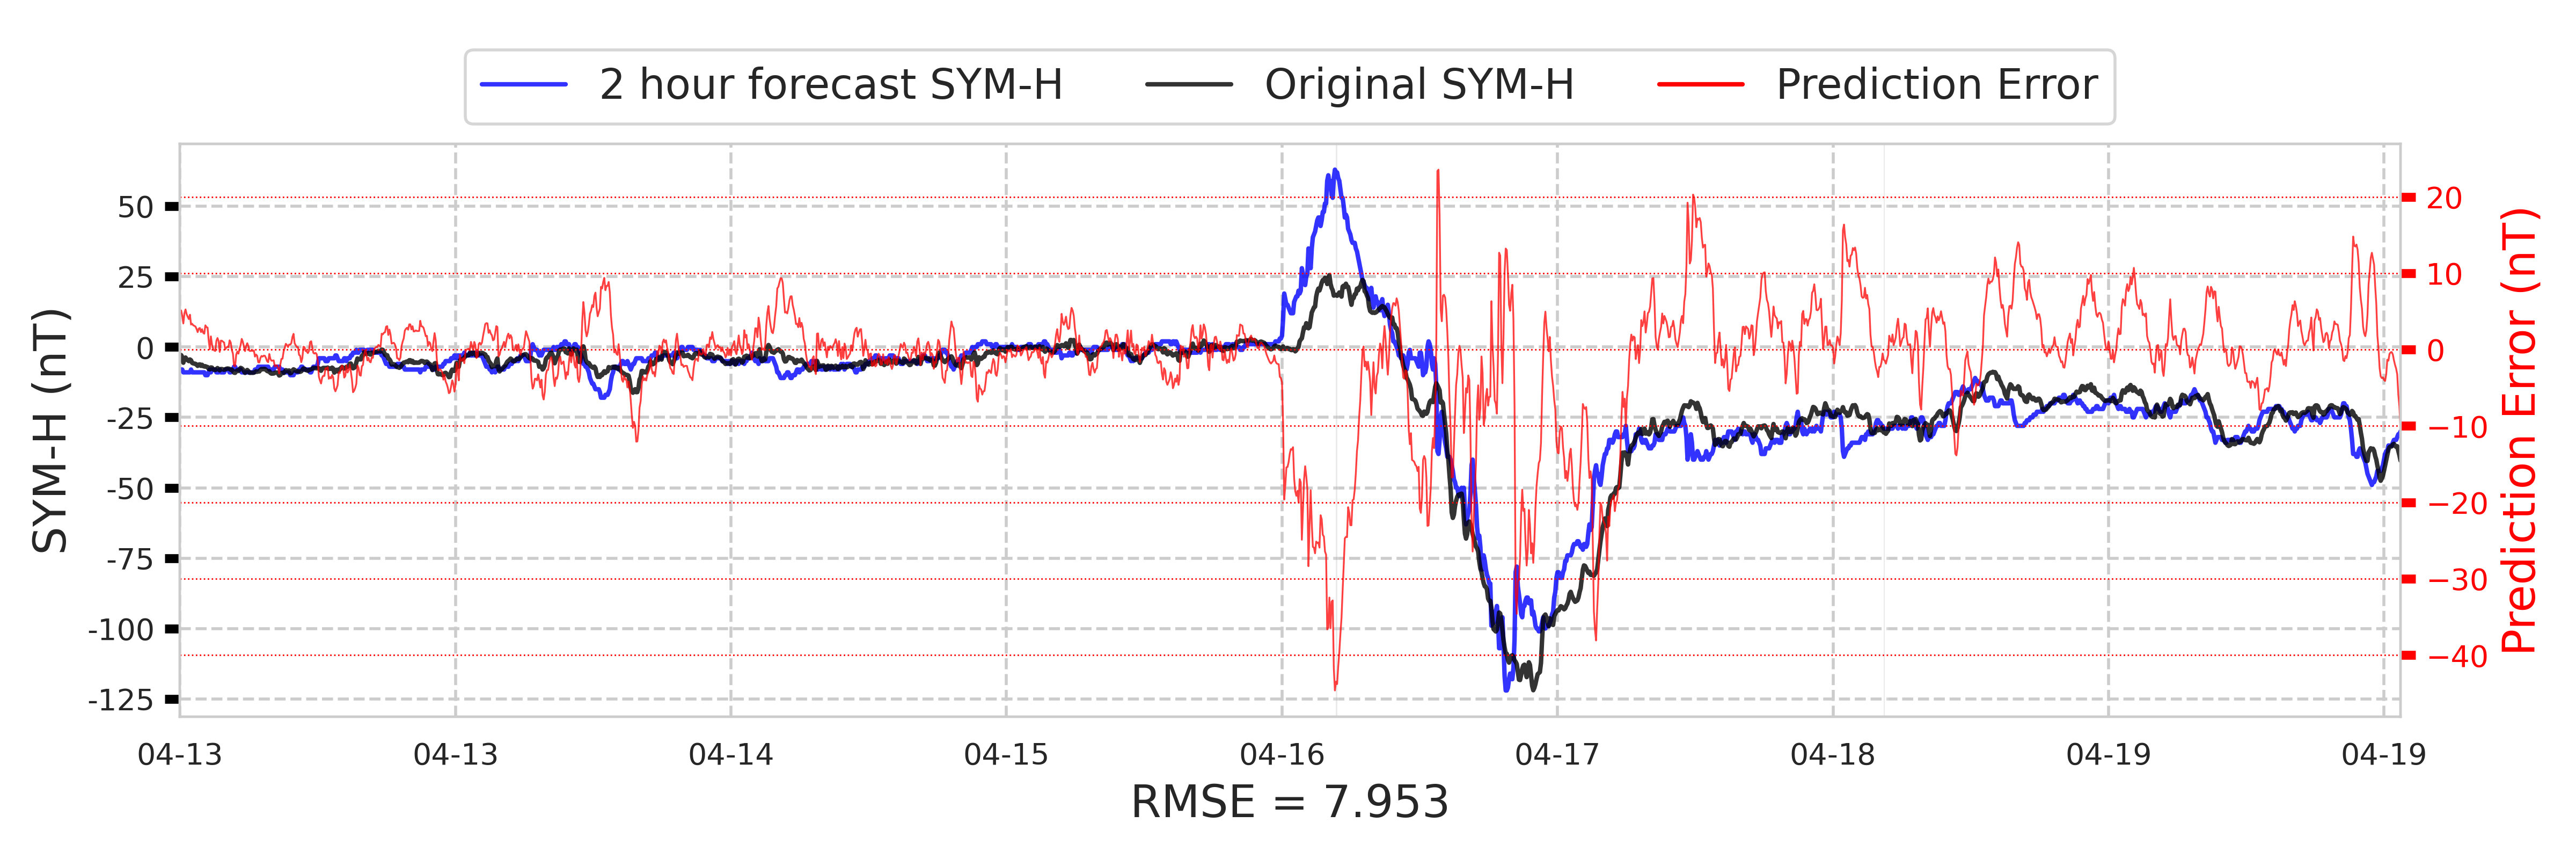
\includegraphics[width=0.49\linewidth]{paper_plots_shade/2h_swics/2h_swics_storm_29.png}
\\
\shortstack{1h forecast using SWICS\\ in laboratory conditions} & \shortstack{2h forecast using SWICS\\ in laboratory conditions}
\vspace*{12pt}
\\
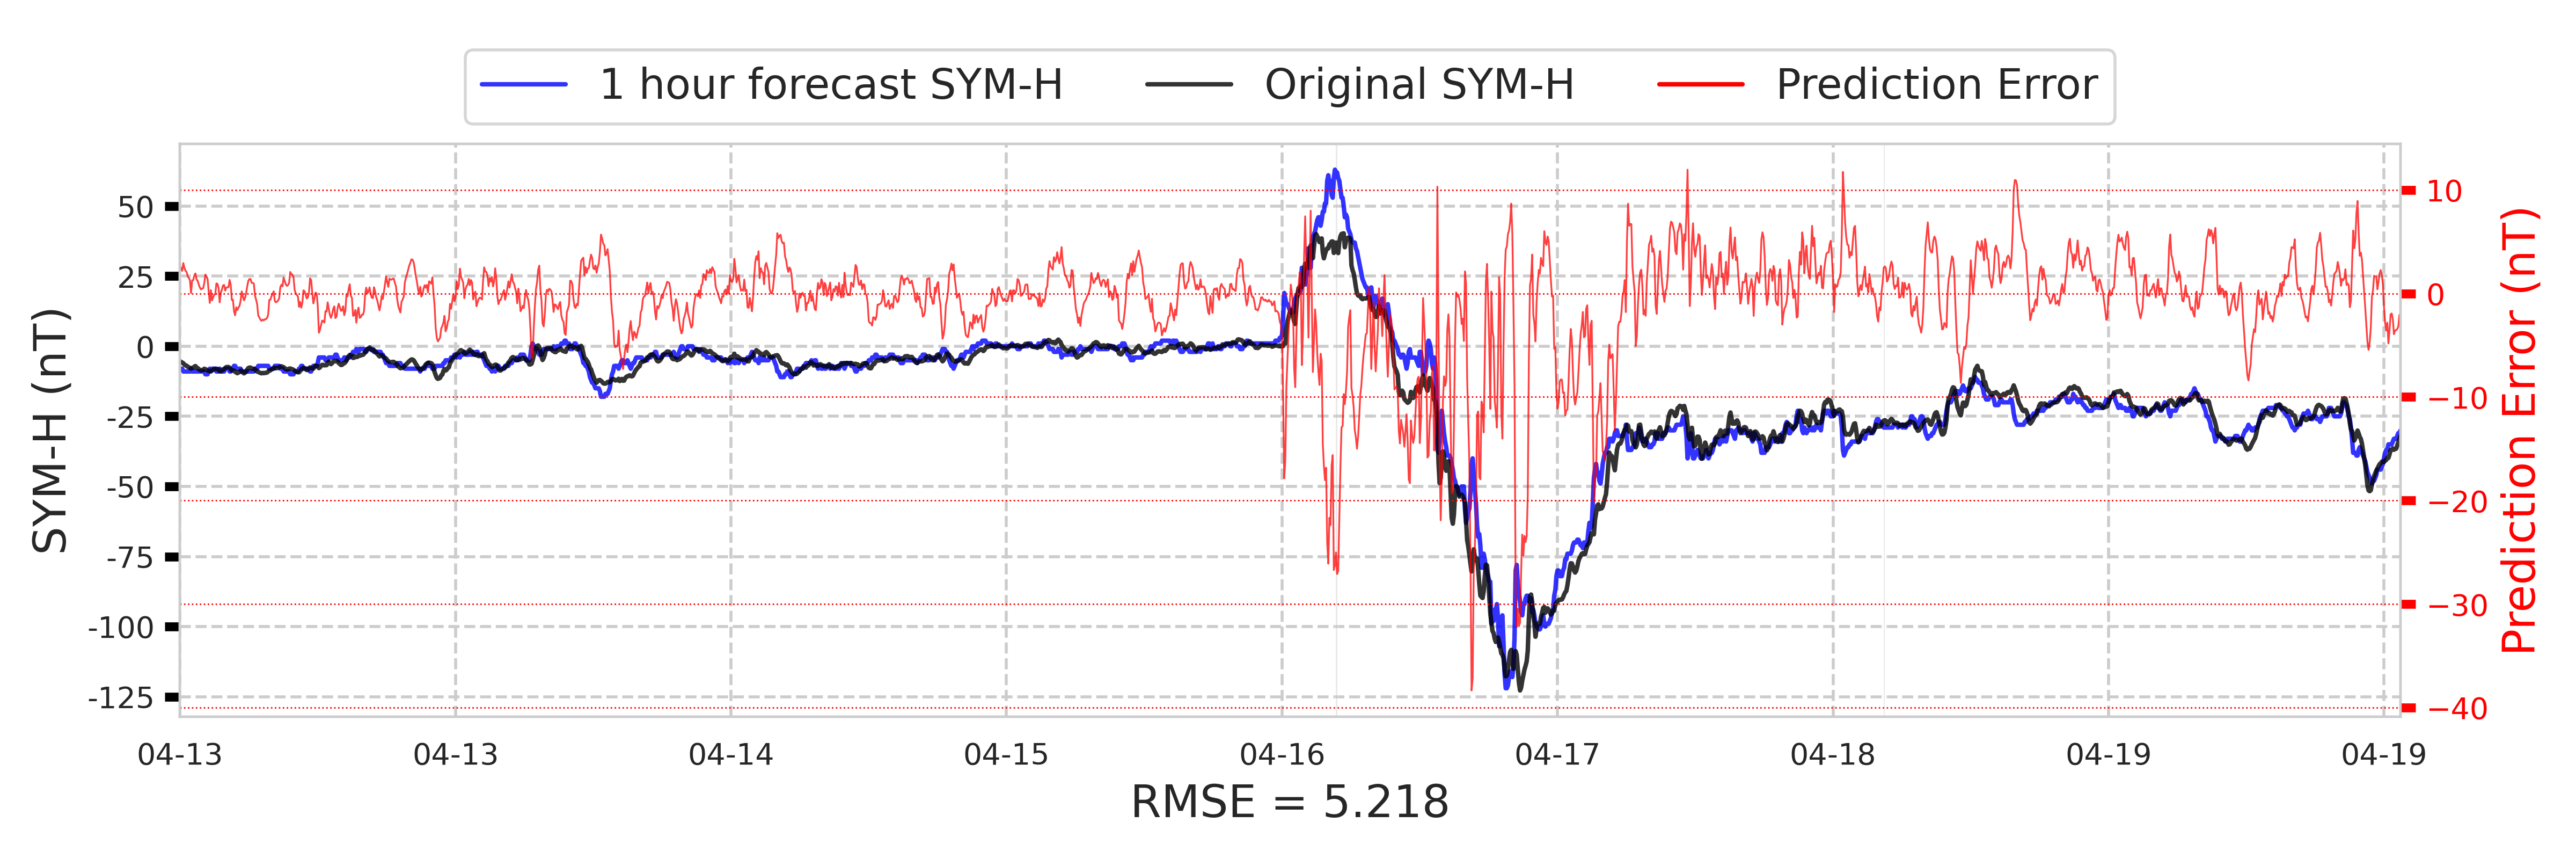
\includegraphics[width=0.49\linewidth]{paper_plots_shade/1h_swics_rt/1h_swics_rt_storm_29.png}
&
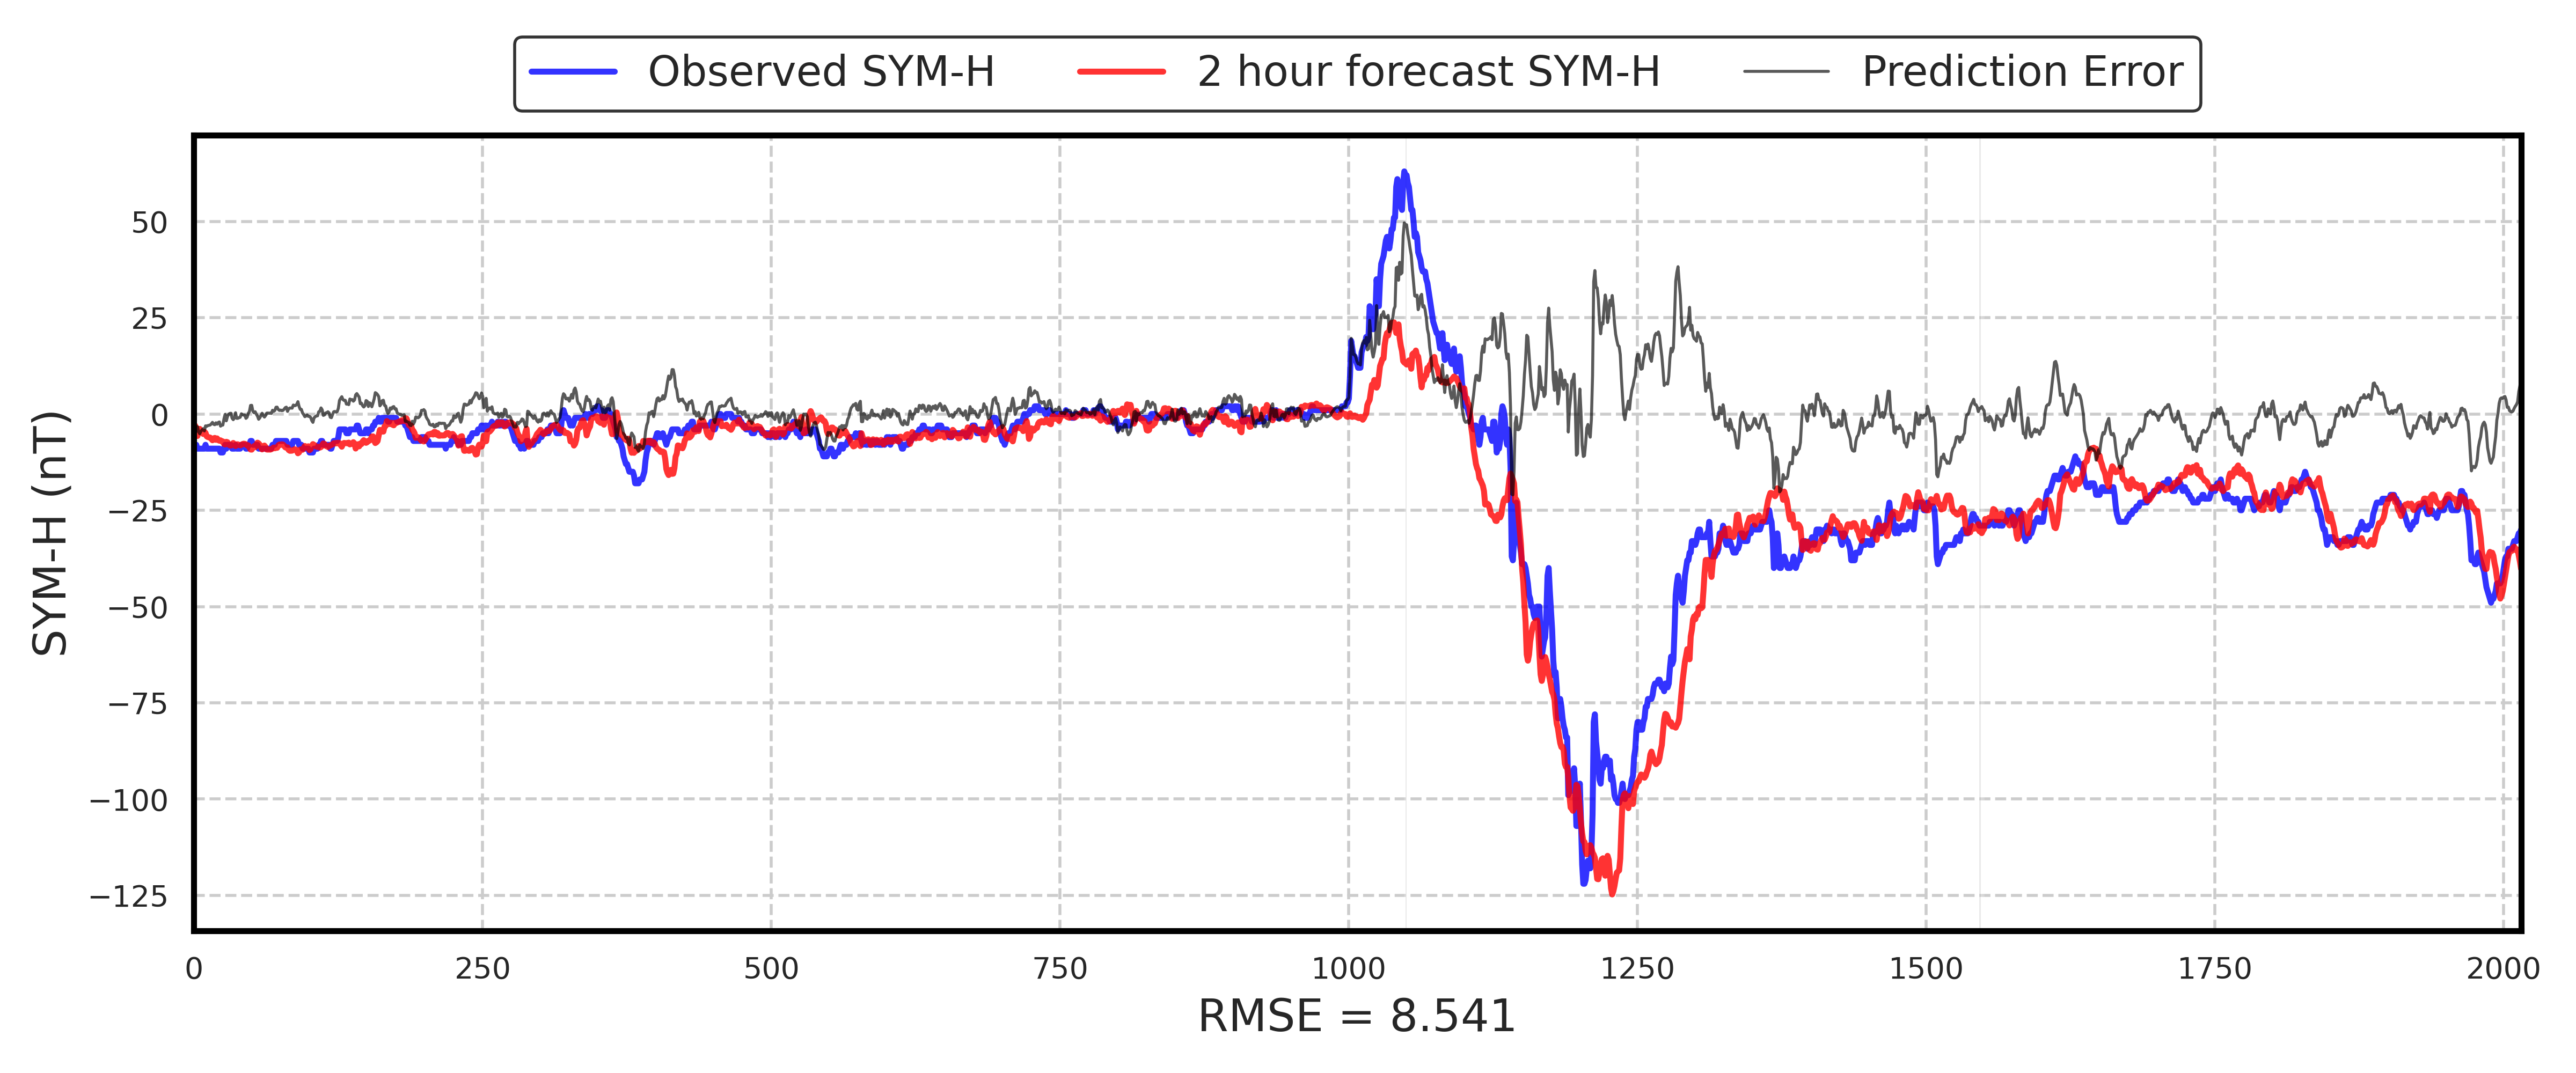
\includegraphics[width=0.49\linewidth]{paper_plots_shade/2h_swics_rt/2h_swics_rt_storm_29.png}
\\
\shortstack{1h operational forecast trained\\ with SWEPAM and SWICS data} & \shortstack{2h operational forecast trained\\ with SWEPAM and SWICS data}
\vspace*{12pt}
\\
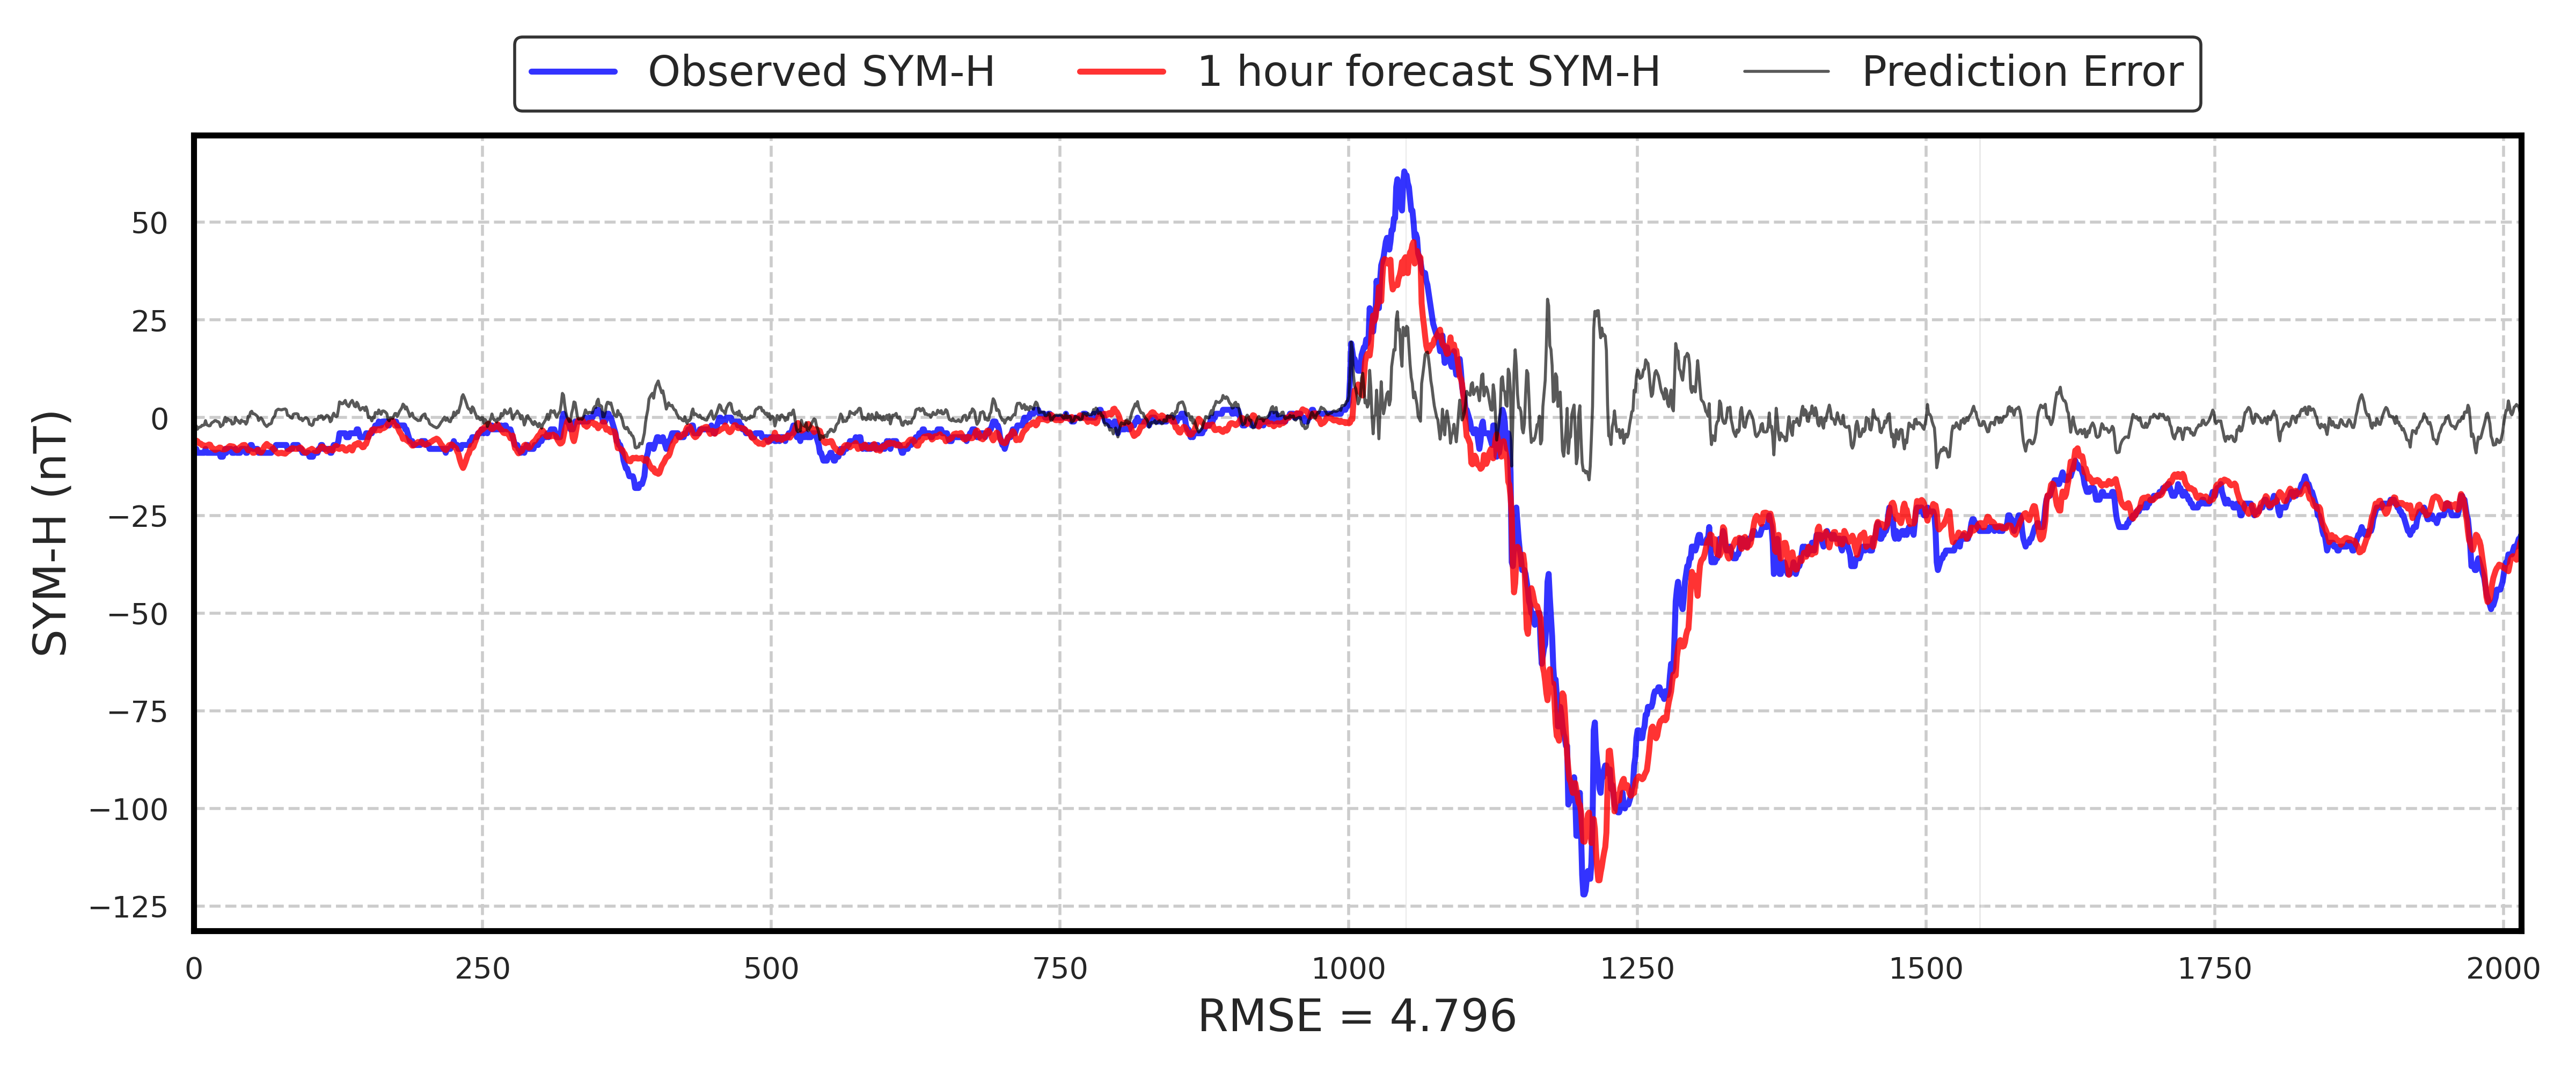
\includegraphics[width=0.49\linewidth]{paper_plots_shade/1h_swepam_rt/1h_swepam_rt_storm_29.png}
&
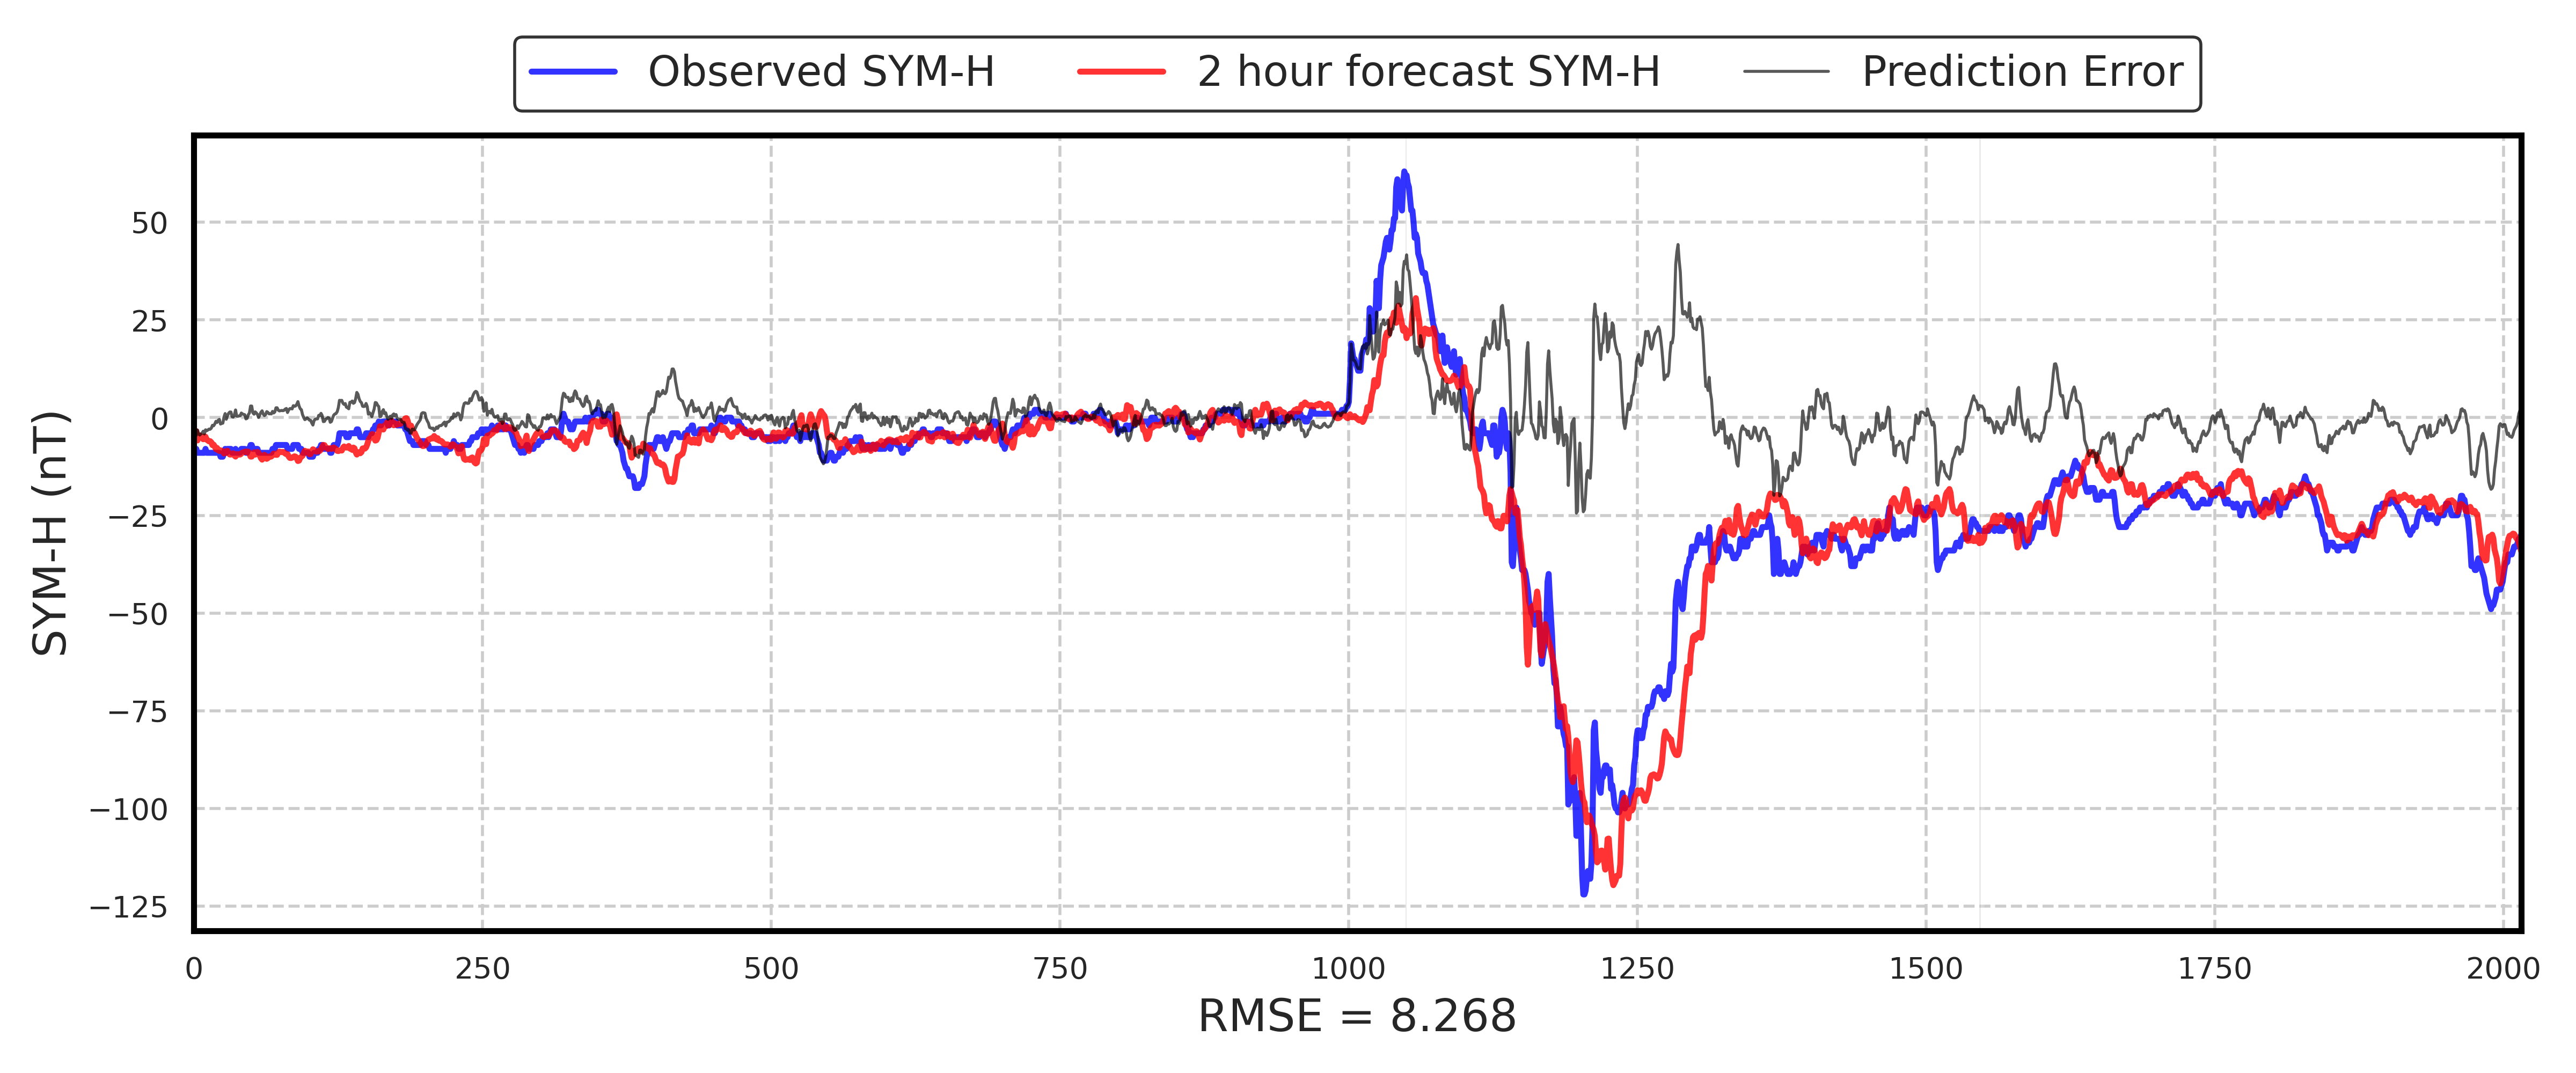
\includegraphics[width=0.49\linewidth]{paper_plots_shade/2h_swepam_rt/2h_swepam_rt_storm_29.png}
\\
\shortstack{1h operational forecast trained\\ with SWEPAM data only} & \shortstack{2h operational forecast trained\\ with SWEPAM data only}
\vspace*{12pt}
\\
\end{tabular}
\caption{Predictions for Storm Number 29 -- April of 1999}
\label{storm-29}
\end{table}



% Figure for storm 30
\begin{table}
\centering
\begin{tabular}{cc}
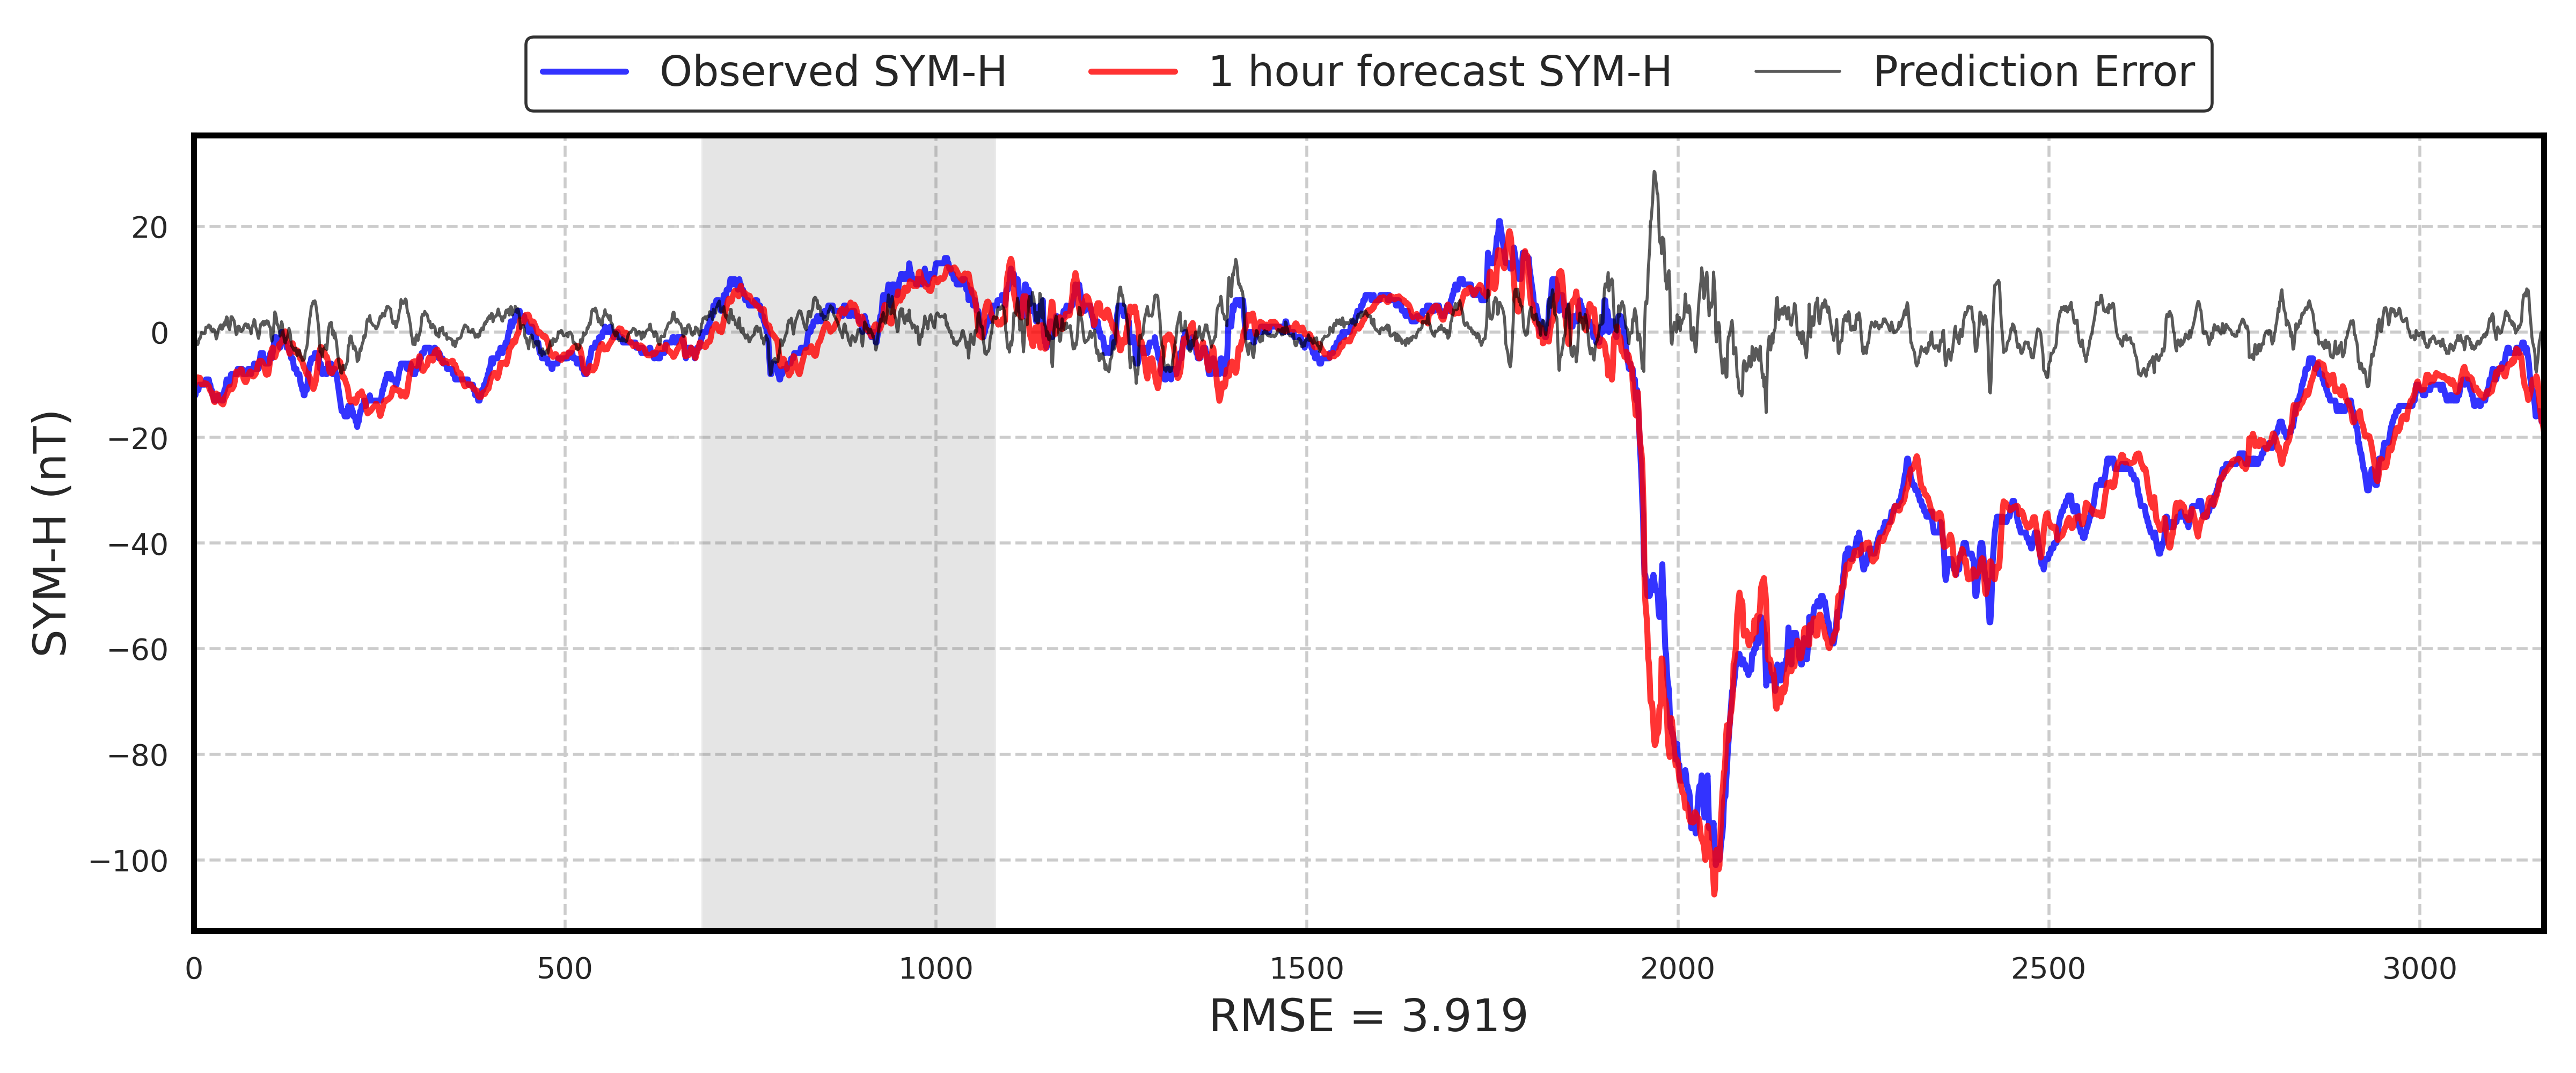
\includegraphics[width=0.49\linewidth]{paper_plots_shade/1h_swics/1h_swics_storm_30.png}
&
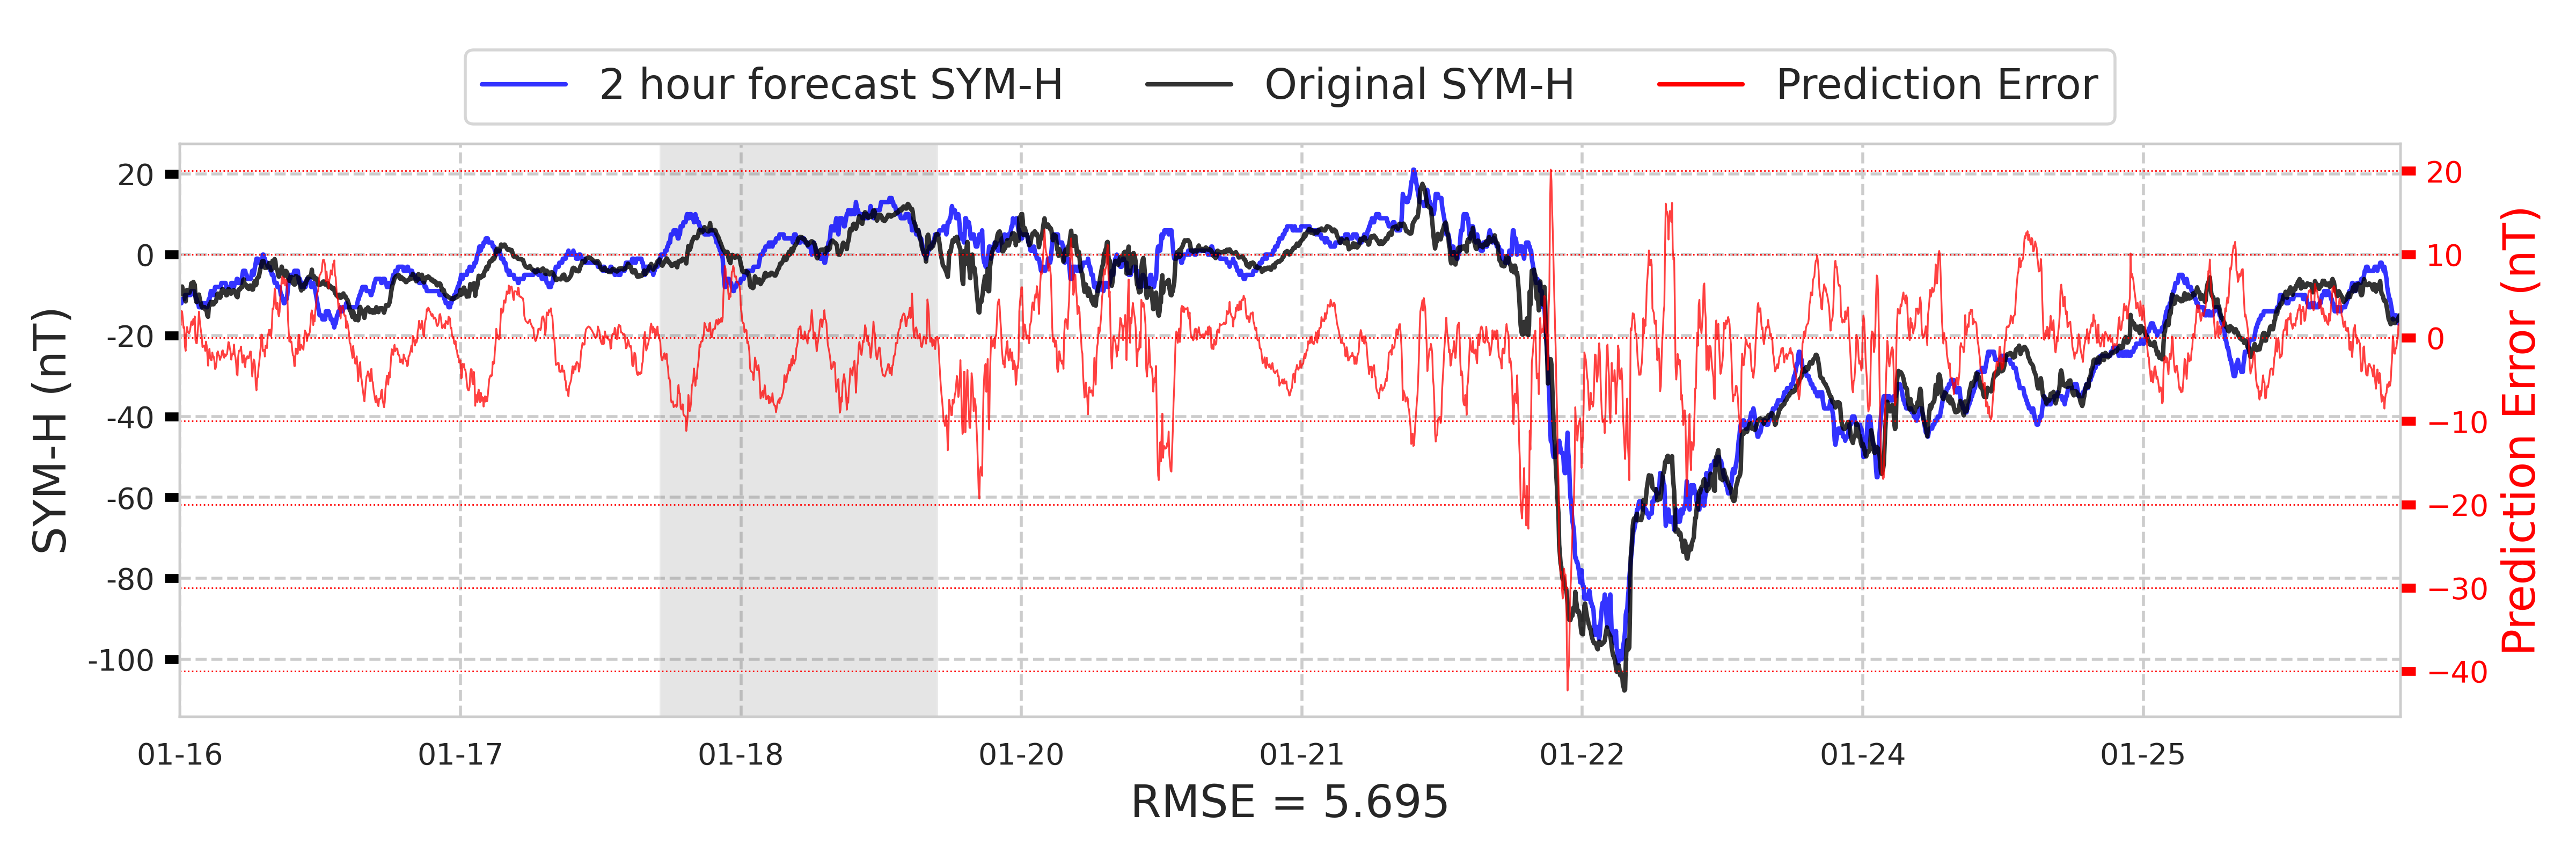
\includegraphics[width=0.49\linewidth]{paper_plots_shade/2h_swics/2h_swics_storm_30.png}
\\
\shortstack{1h forecast using SWICS\\ in laboratory conditions} & \shortstack{2h forecast using SWICS\\ in laboratory conditions}
\vspace*{12pt}
\\
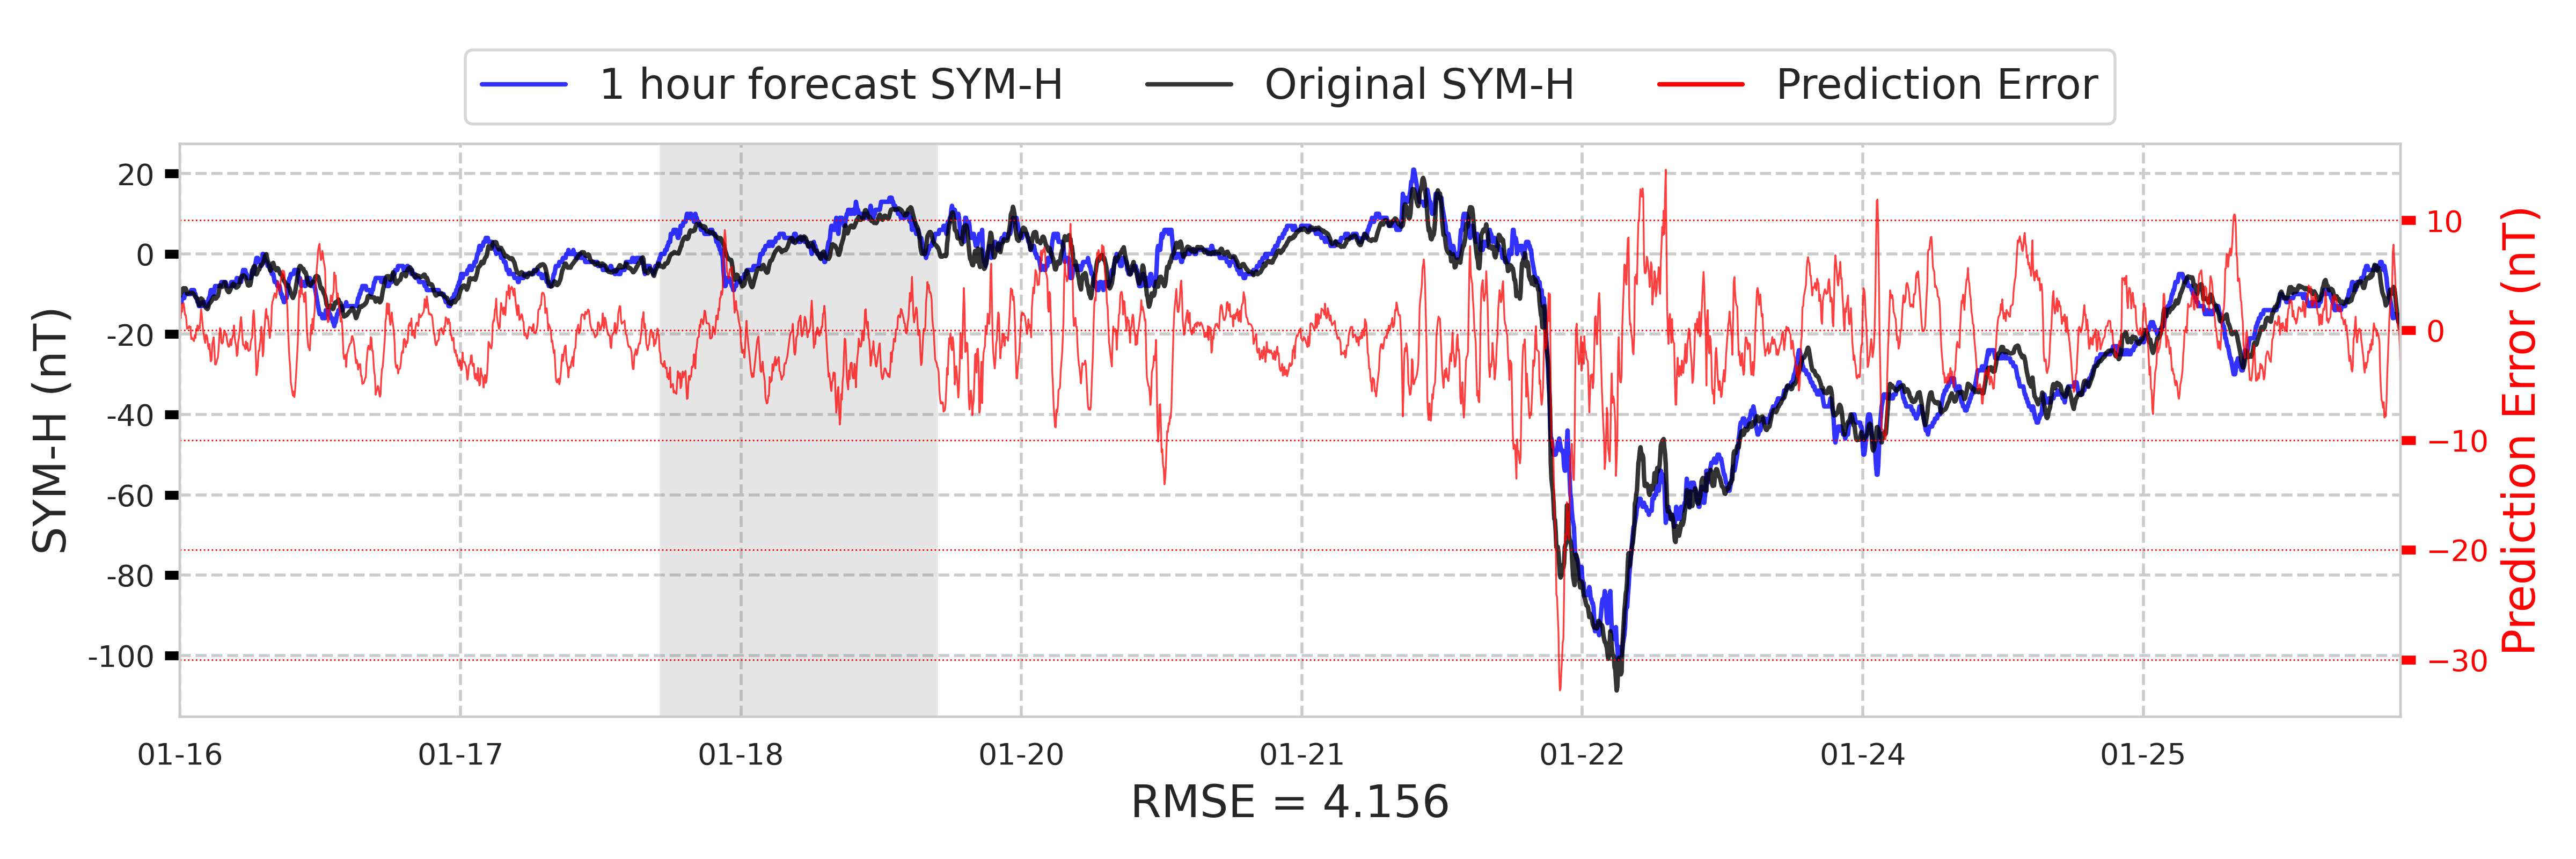
\includegraphics[width=0.49\linewidth]{paper_plots_shade/1h_swics_rt/1h_swics_rt_storm_30.png}
&
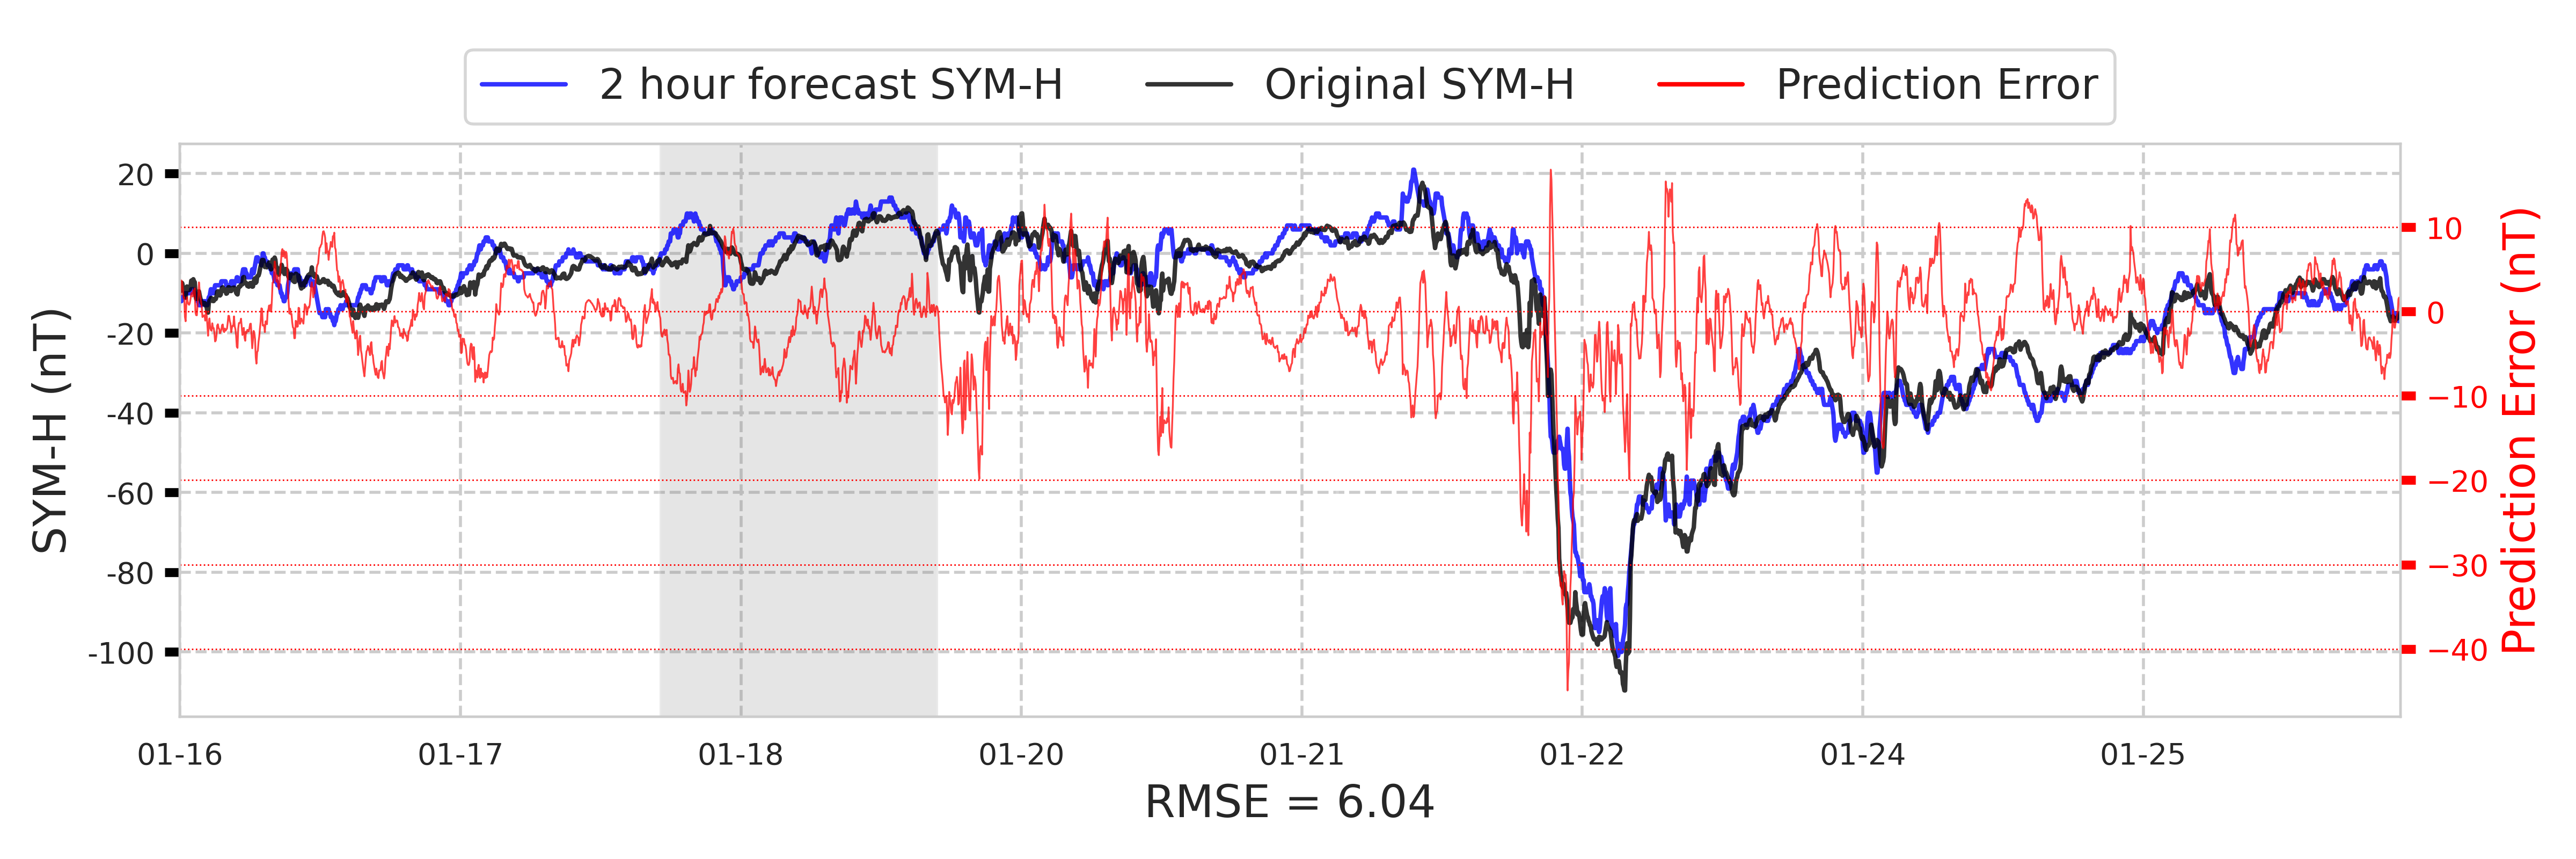
\includegraphics[width=0.49\linewidth]{paper_plots_shade/2h_swics_rt/2h_swics_rt_storm_30.png}
\\
\shortstack{1h operational forecast trained\\ with SWEPAM and SWICS data} & \shortstack{2h operational forecast trained\\ with SWEPAM and SWICS data}
\vspace*{12pt}
\\
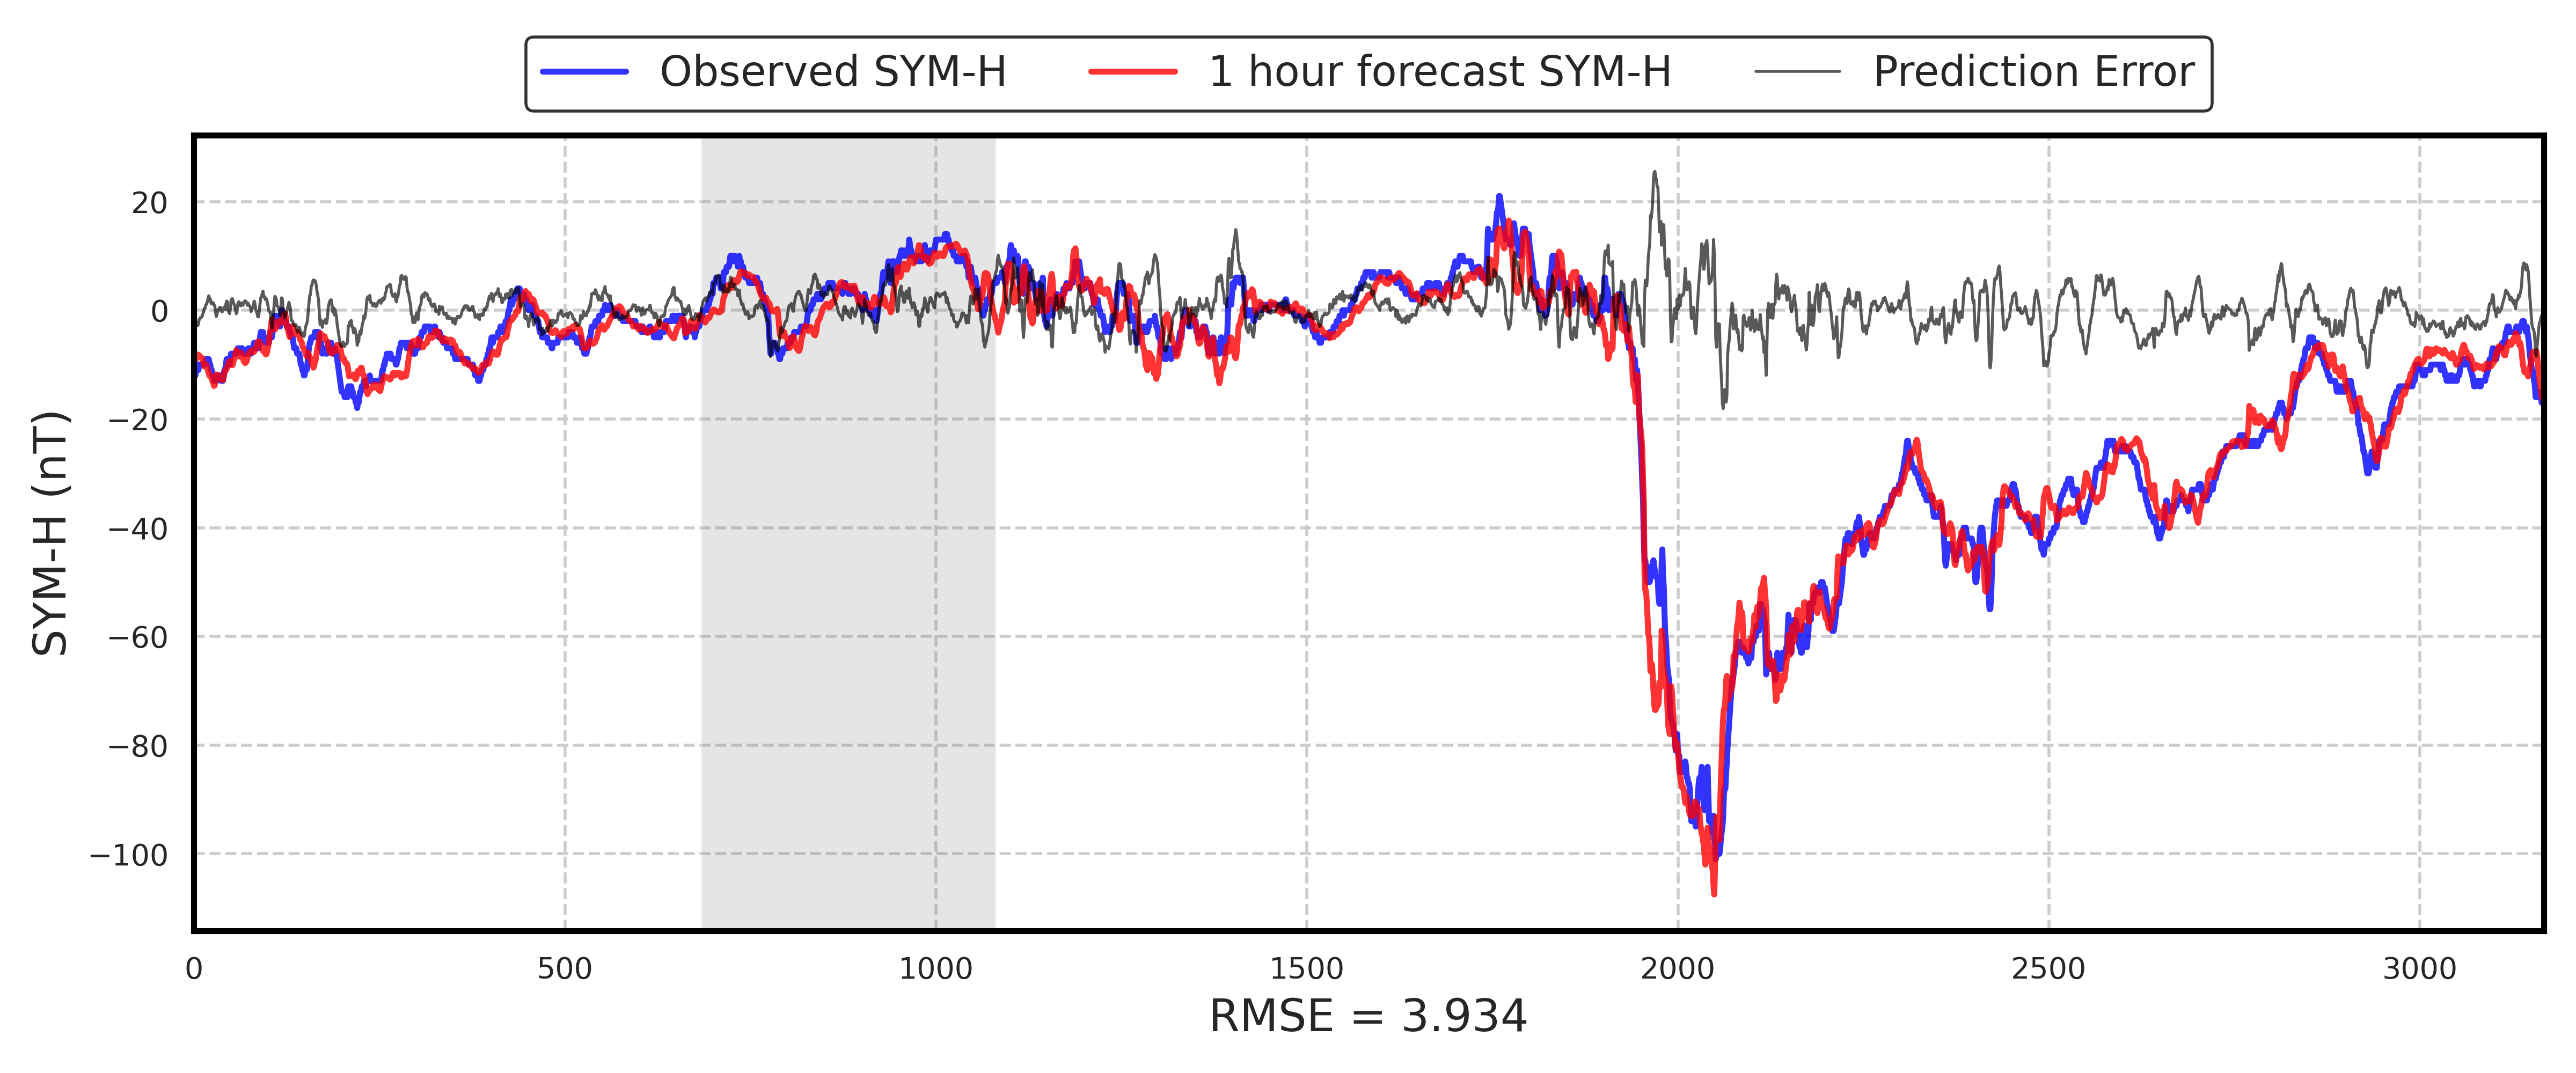
\includegraphics[width=0.49\linewidth]{paper_plots_shade/1h_swepam_rt/1h_swepam_rt_storm_30.png}
&
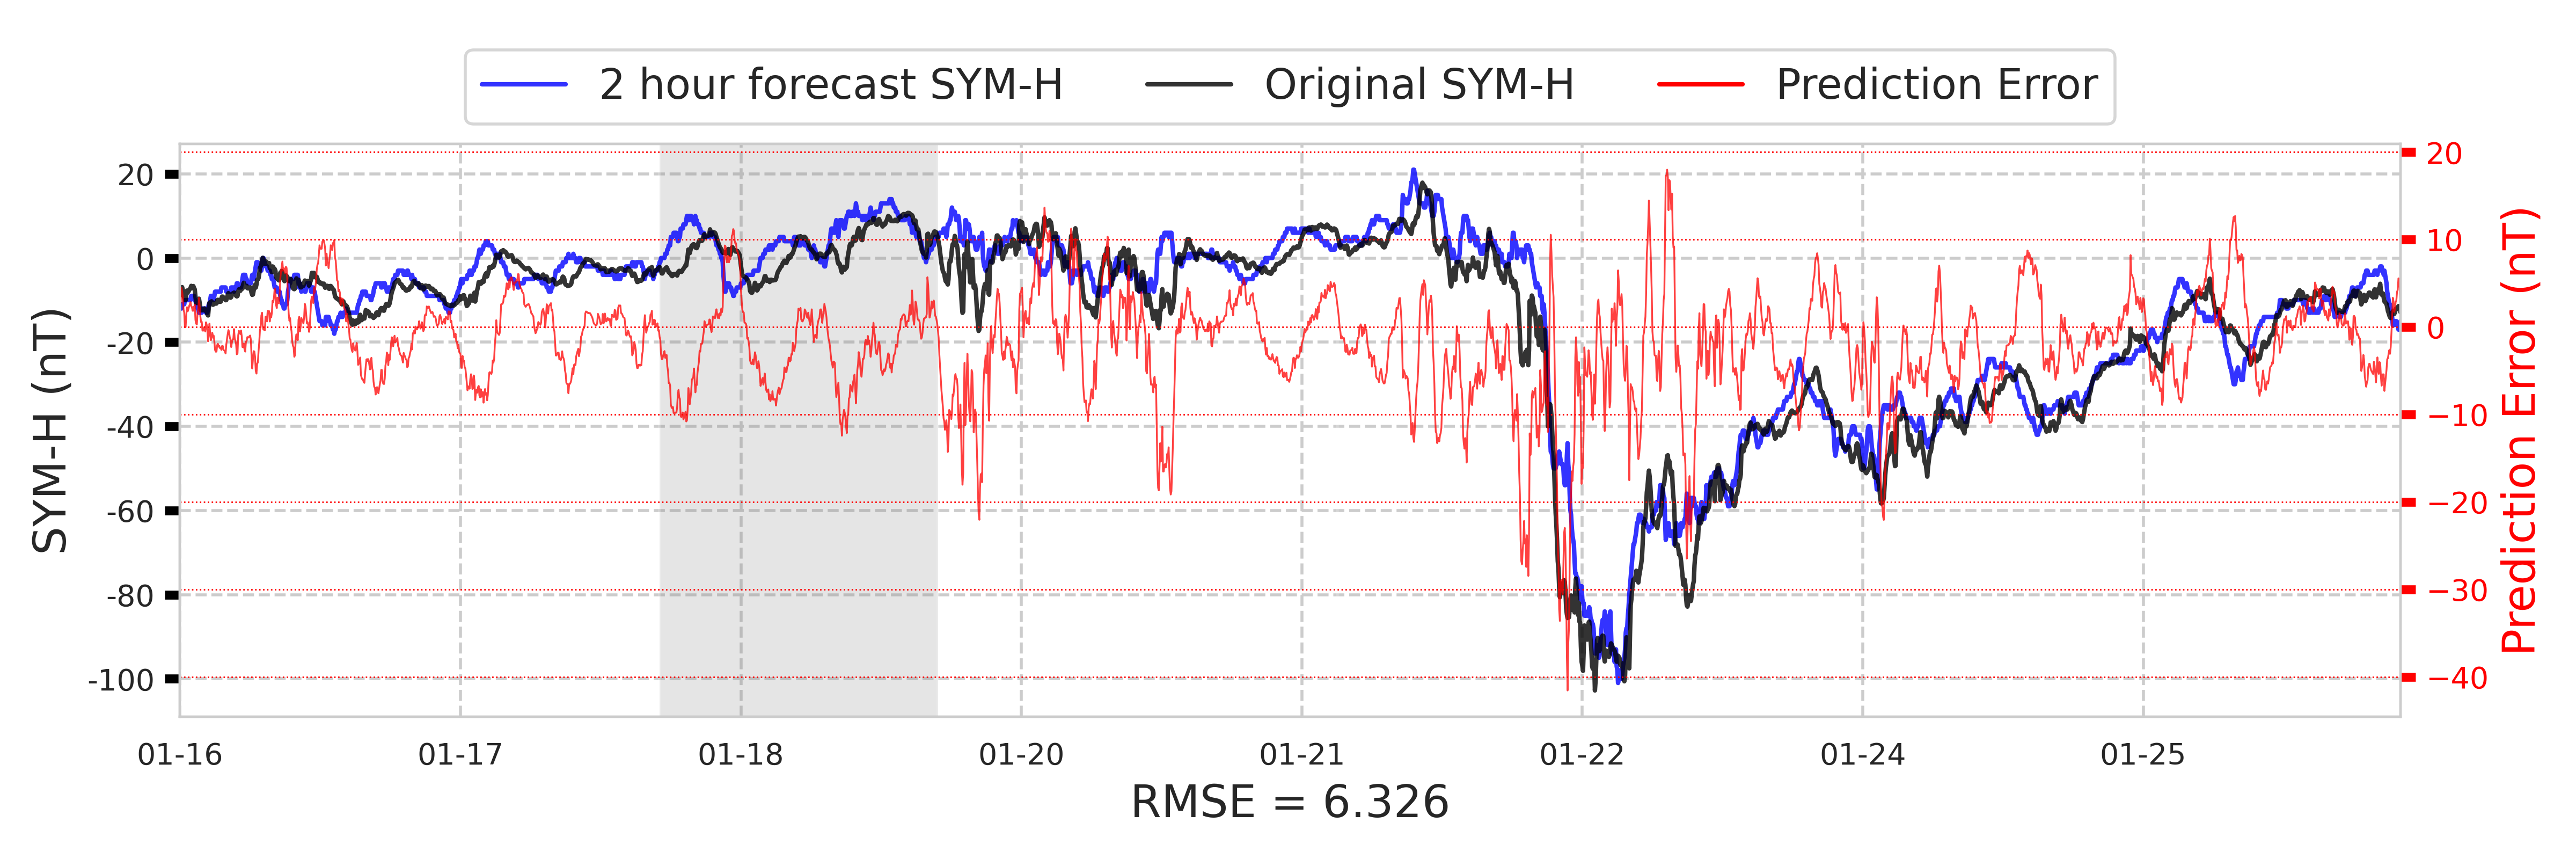
\includegraphics[width=0.49\linewidth]{paper_plots_shade/2h_swepam_rt/2h_swepam_rt_storm_30.png}
\\
\shortstack{1h operational forecast trained\\ with SWEPAM data only} & \shortstack{2h operational forecast trained\\ with SWEPAM data only}
\vspace*{12pt}
\\
\end{tabular}
\caption{Predictions for Storm Number 30 -- January of 2000}
\label{storm-30}
\end{table}



% Figure for storm 31
\begin{table}
\centering
\begin{tabular}{cc}
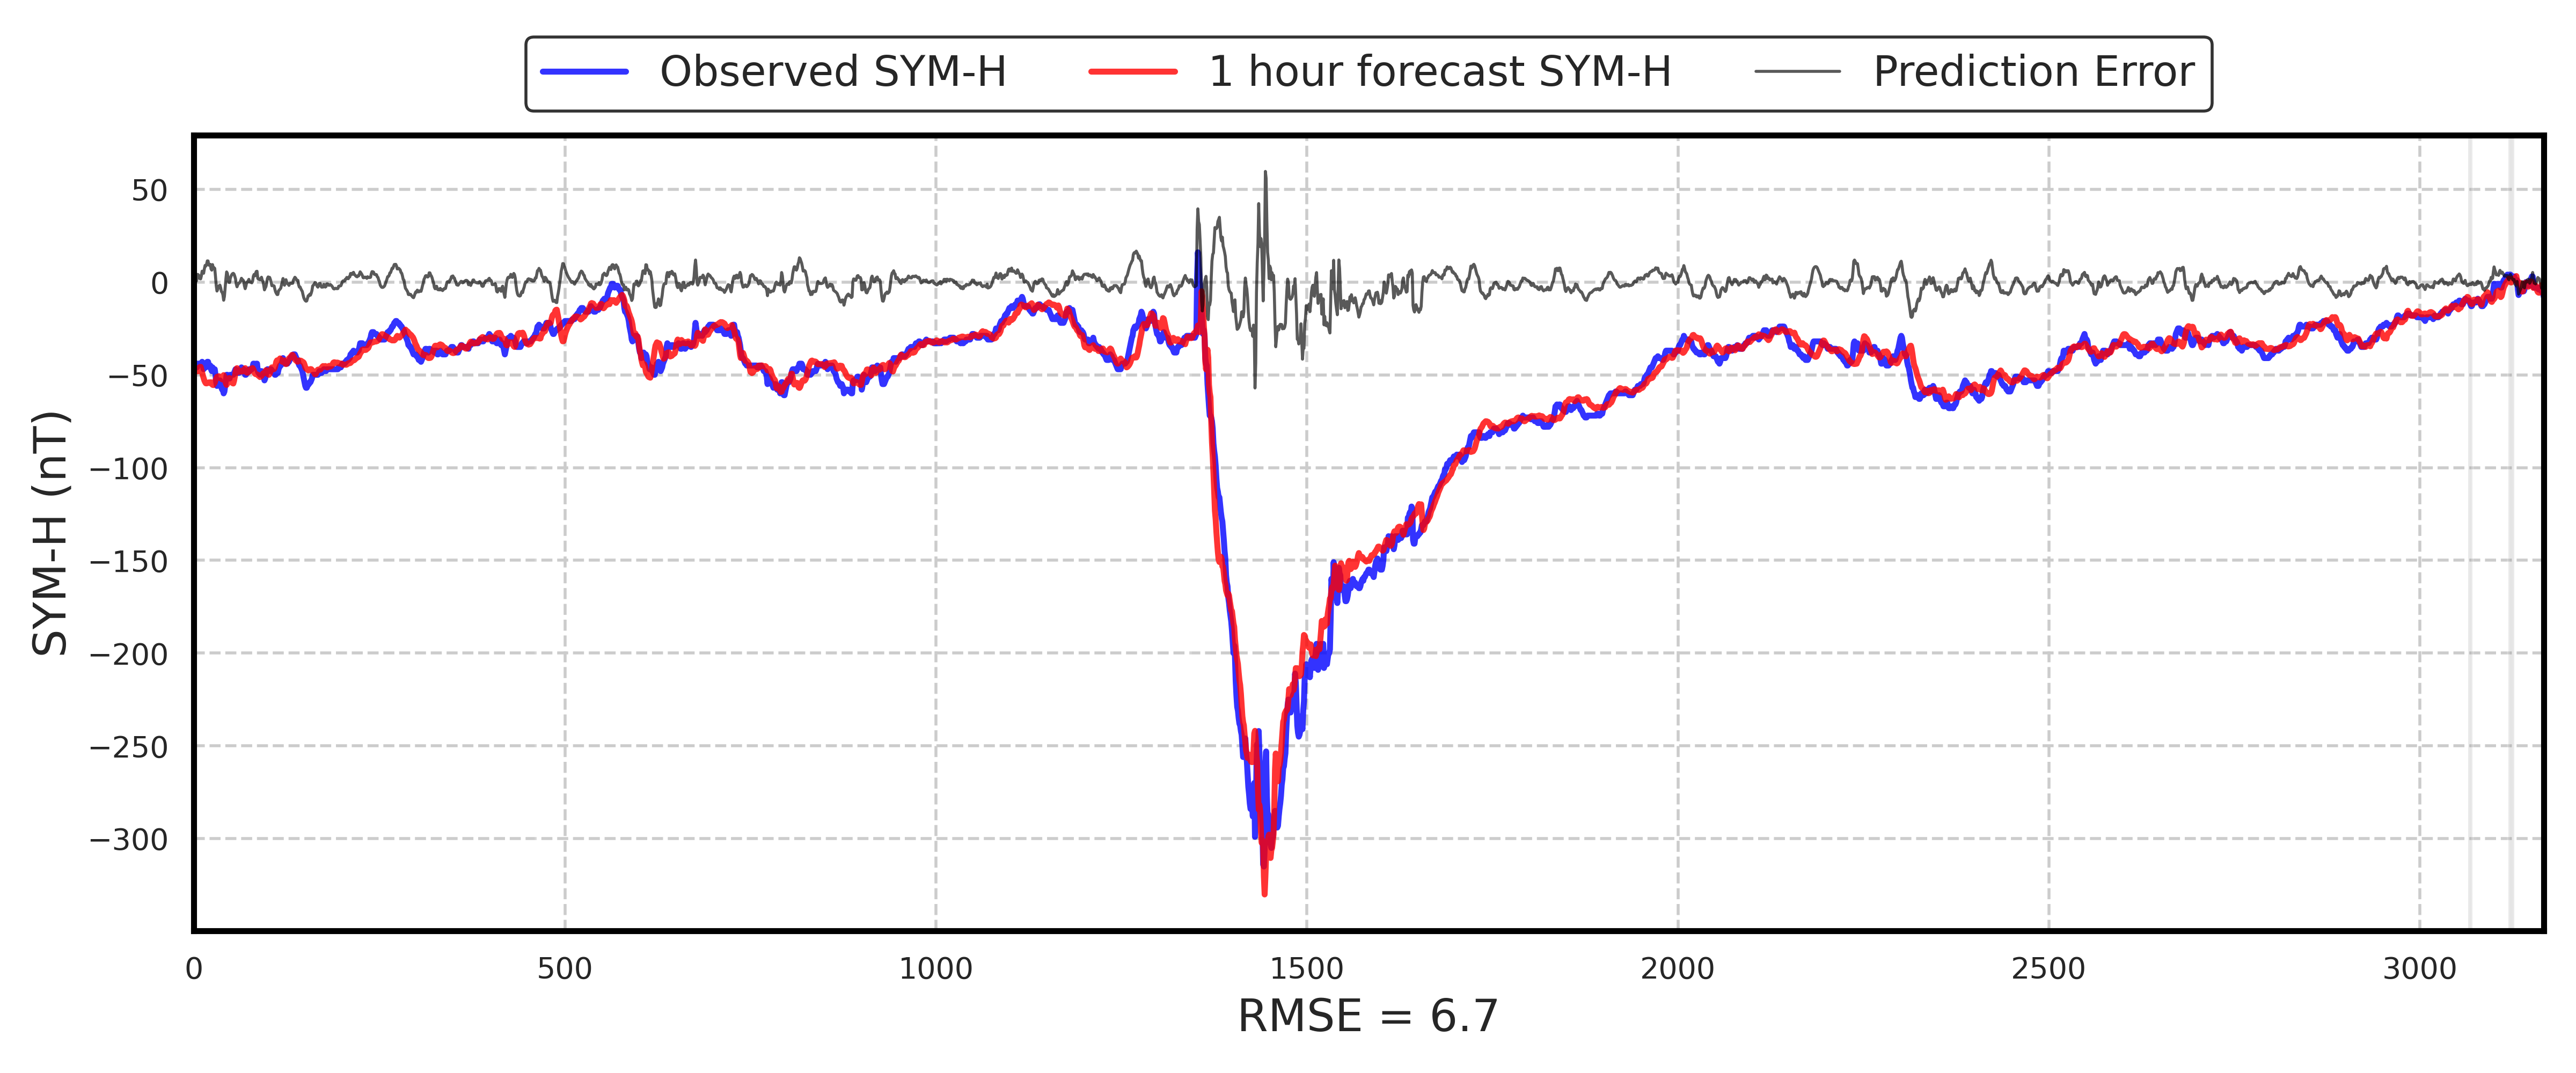
\includegraphics[width=0.49\linewidth]{paper_plots_shade/1h_swics/1h_swics_storm_31.png}
&
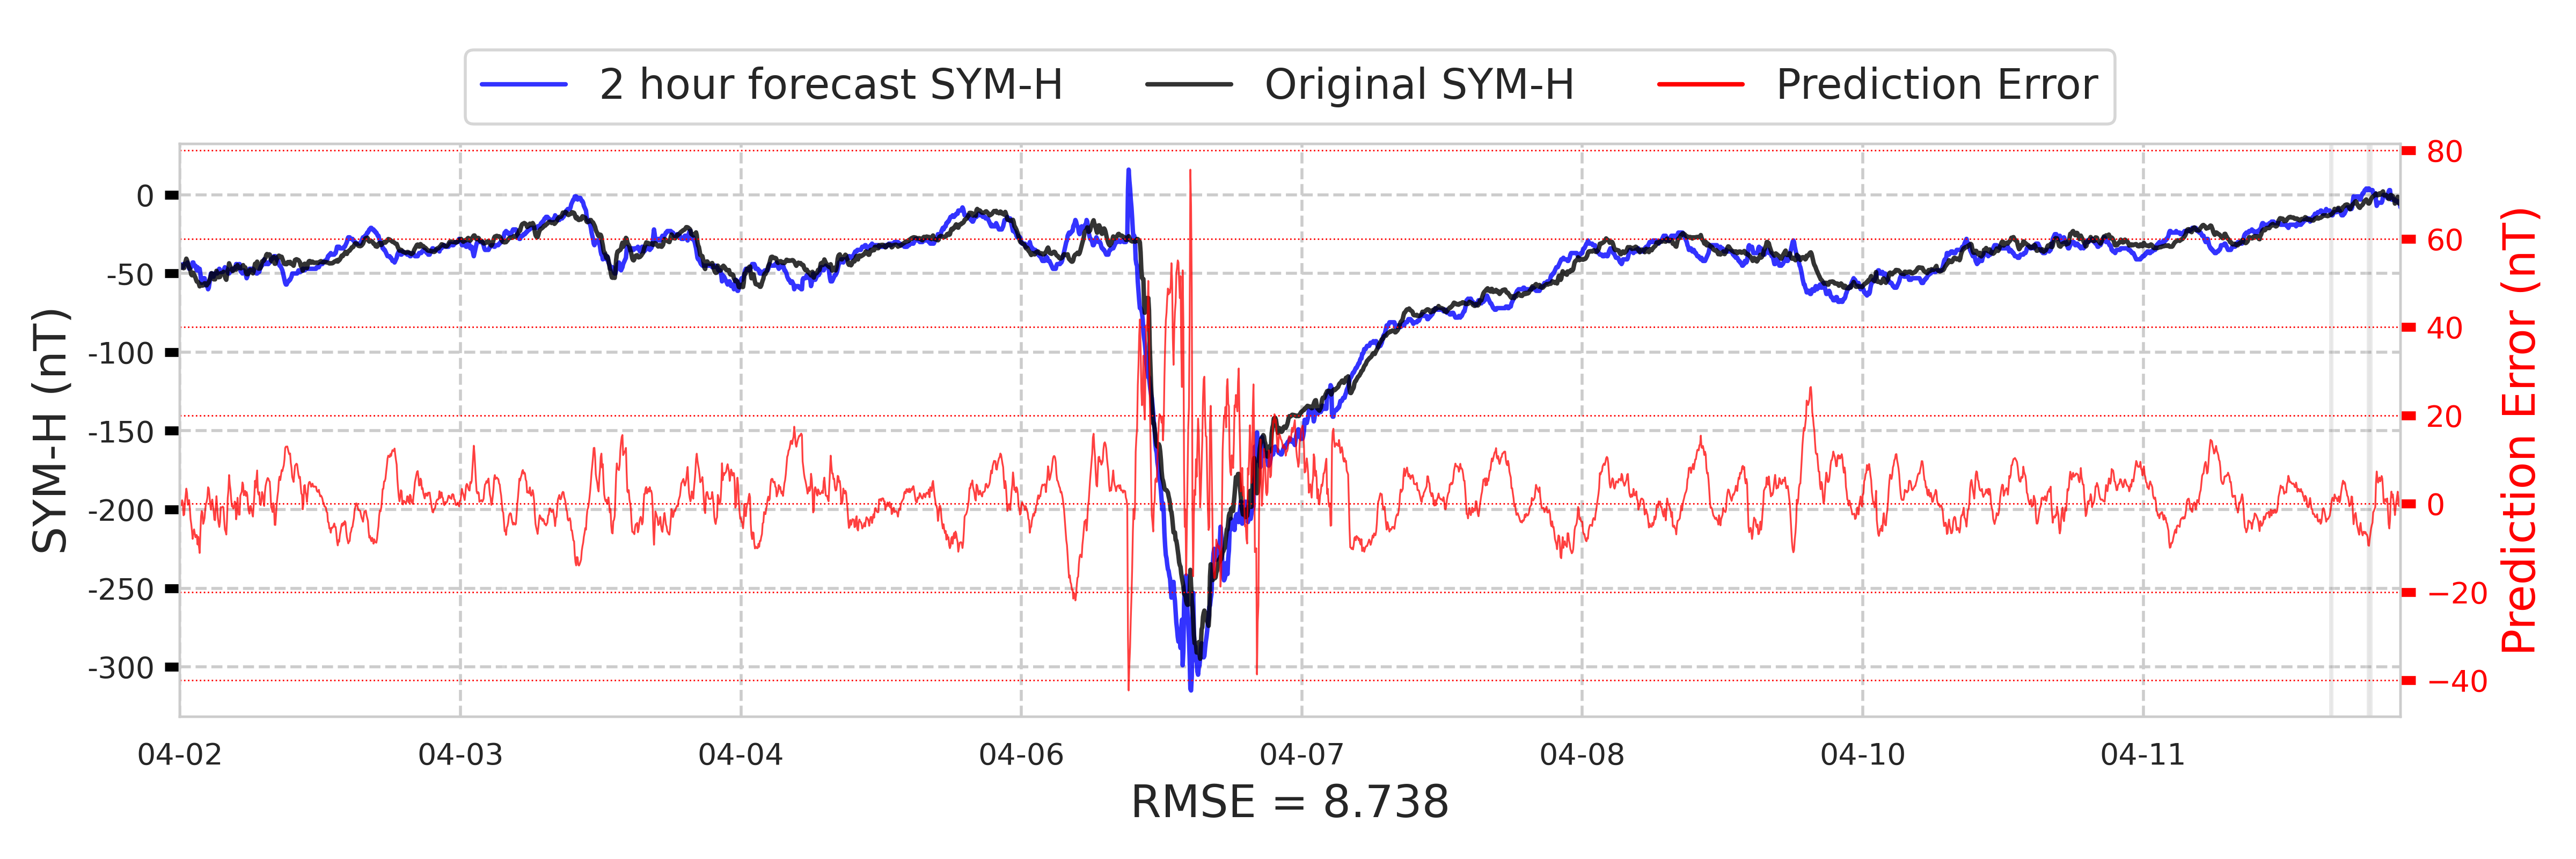
\includegraphics[width=0.49\linewidth]{paper_plots_shade/2h_swics/2h_swics_storm_31.png}
\\
\shortstack{1h forecast using SWICS\\ in laboratory conditions} & \shortstack{2h forecast using SWICS\\ in laboratory conditions}
\vspace*{12pt}
\\
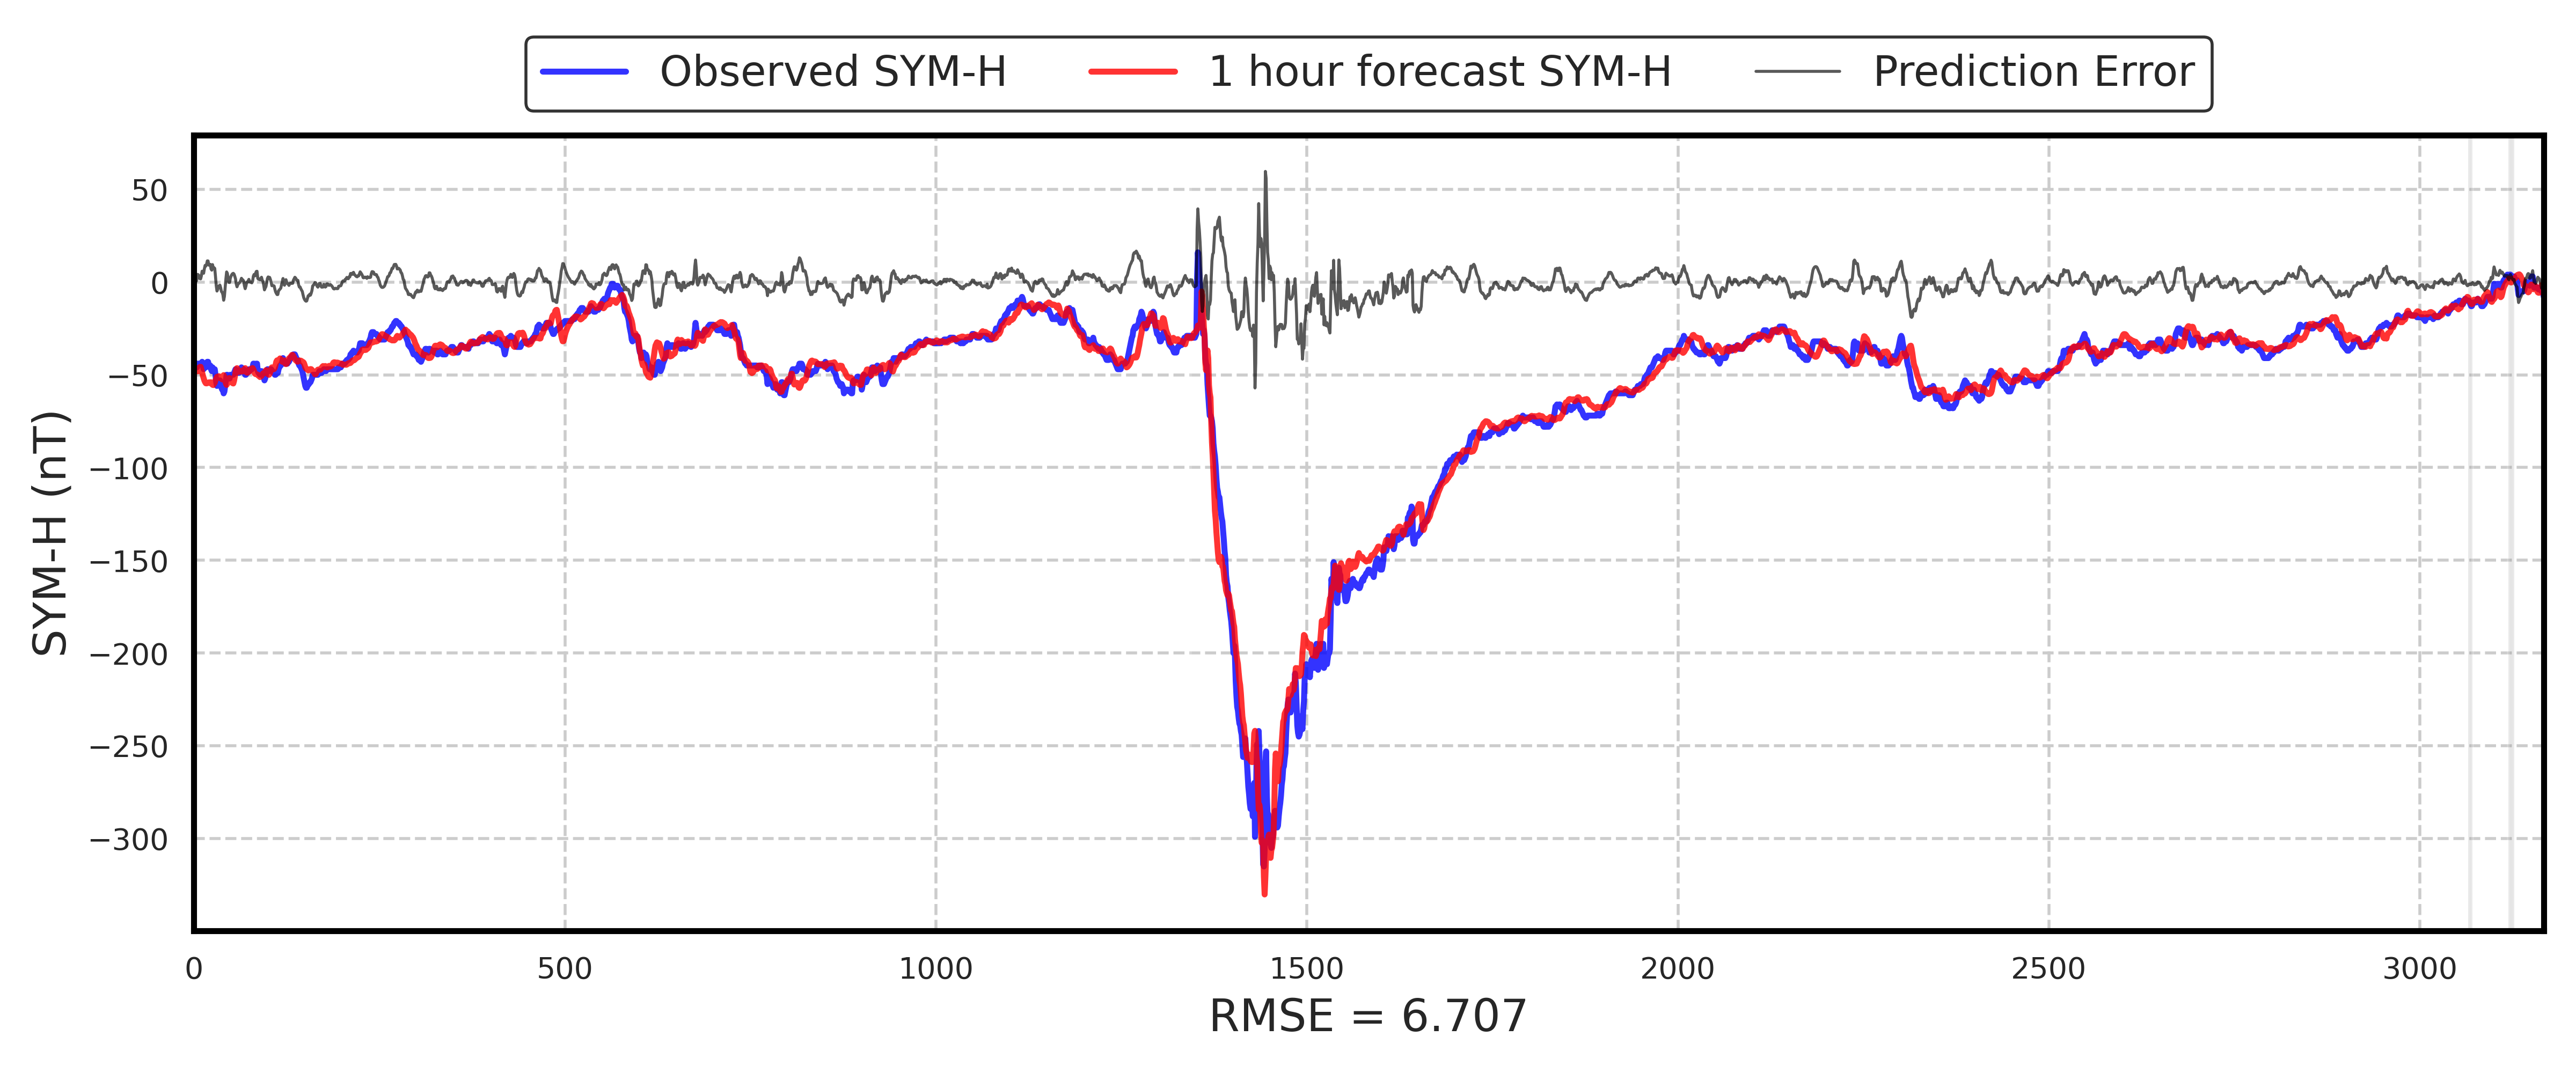
\includegraphics[width=0.49\linewidth]{paper_plots_shade/1h_swics_rt/1h_swics_rt_storm_31.png}
&
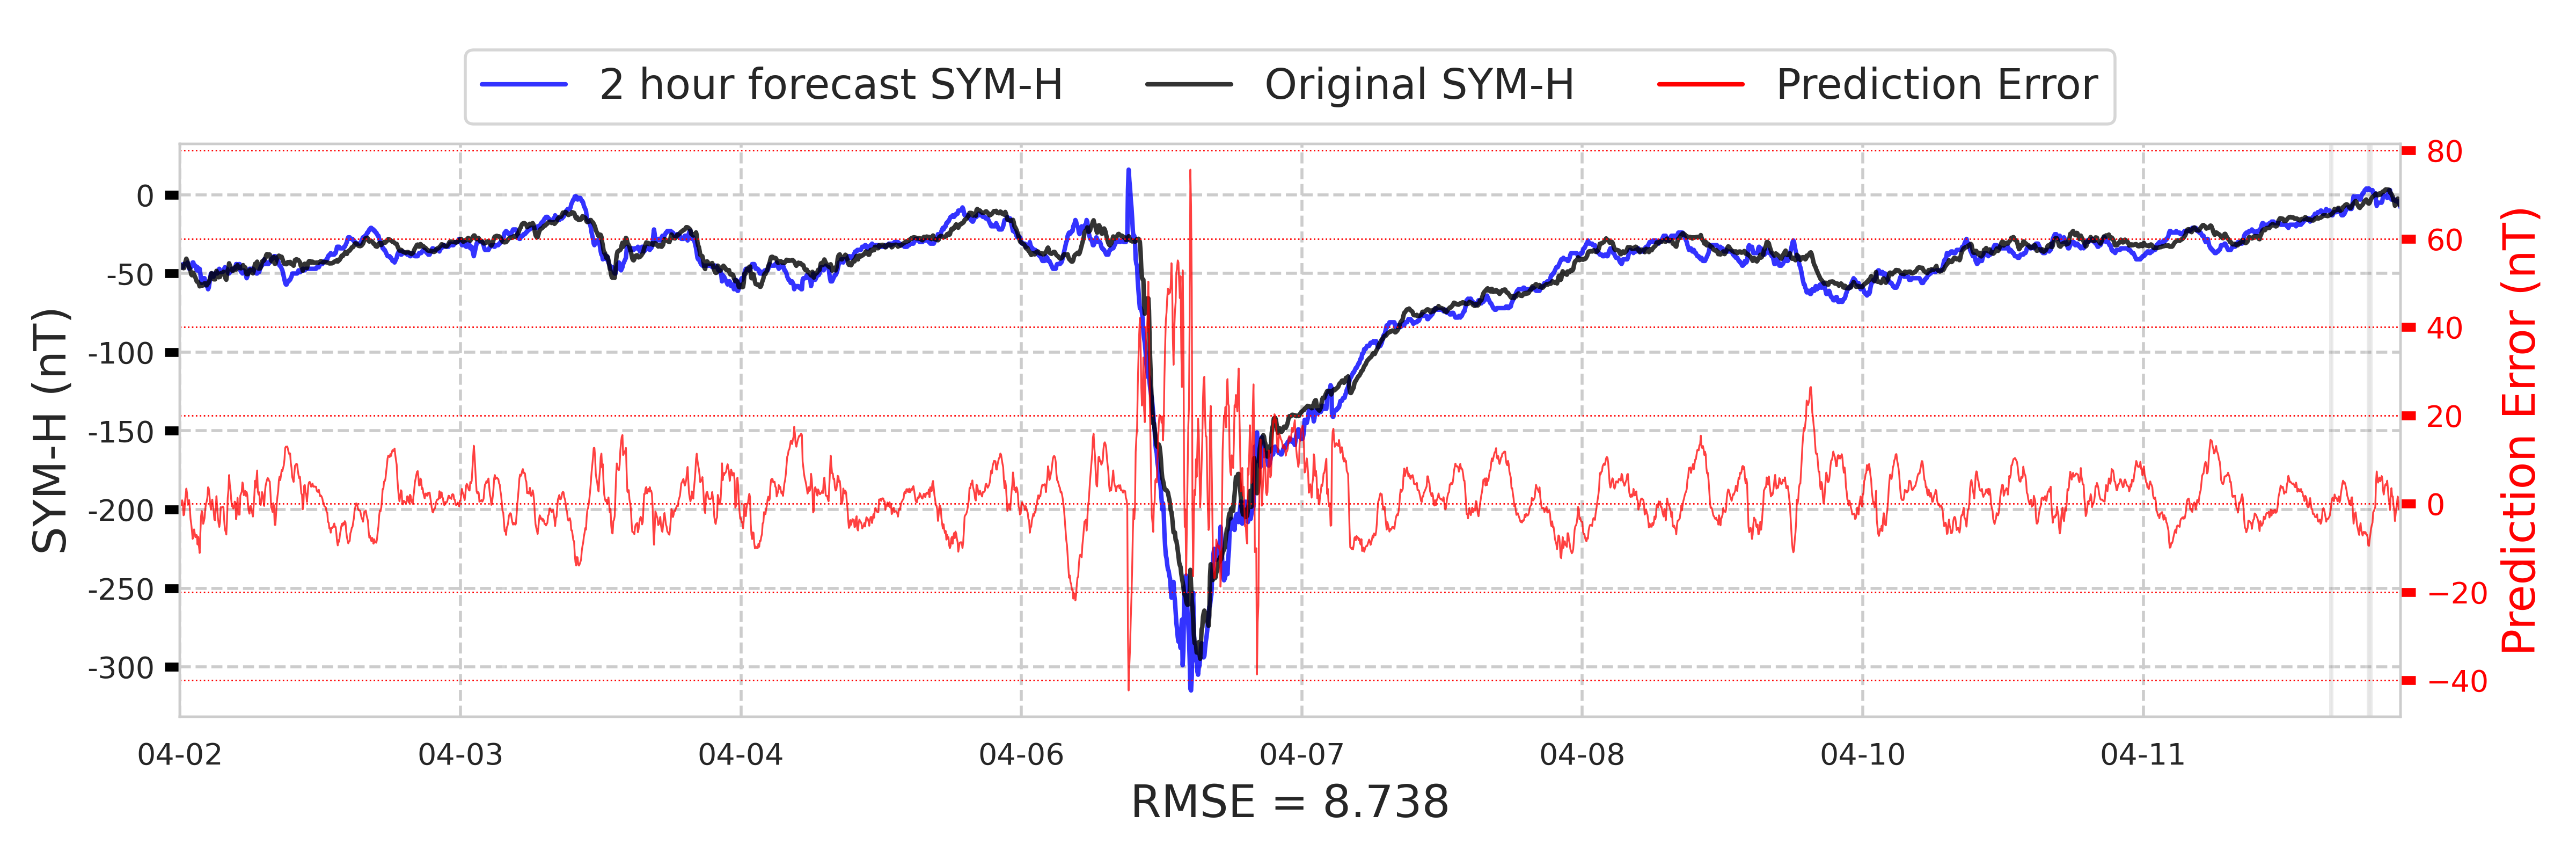
\includegraphics[width=0.49\linewidth]{paper_plots_shade/2h_swics_rt/2h_swics_rt_storm_31.png}
\\
\shortstack{1h operational forecast trained\\ with SWEPAM and SWICS data} & \shortstack{2h operational forecast trained\\ with SWEPAM and SWICS data}
\vspace*{12pt}
\\
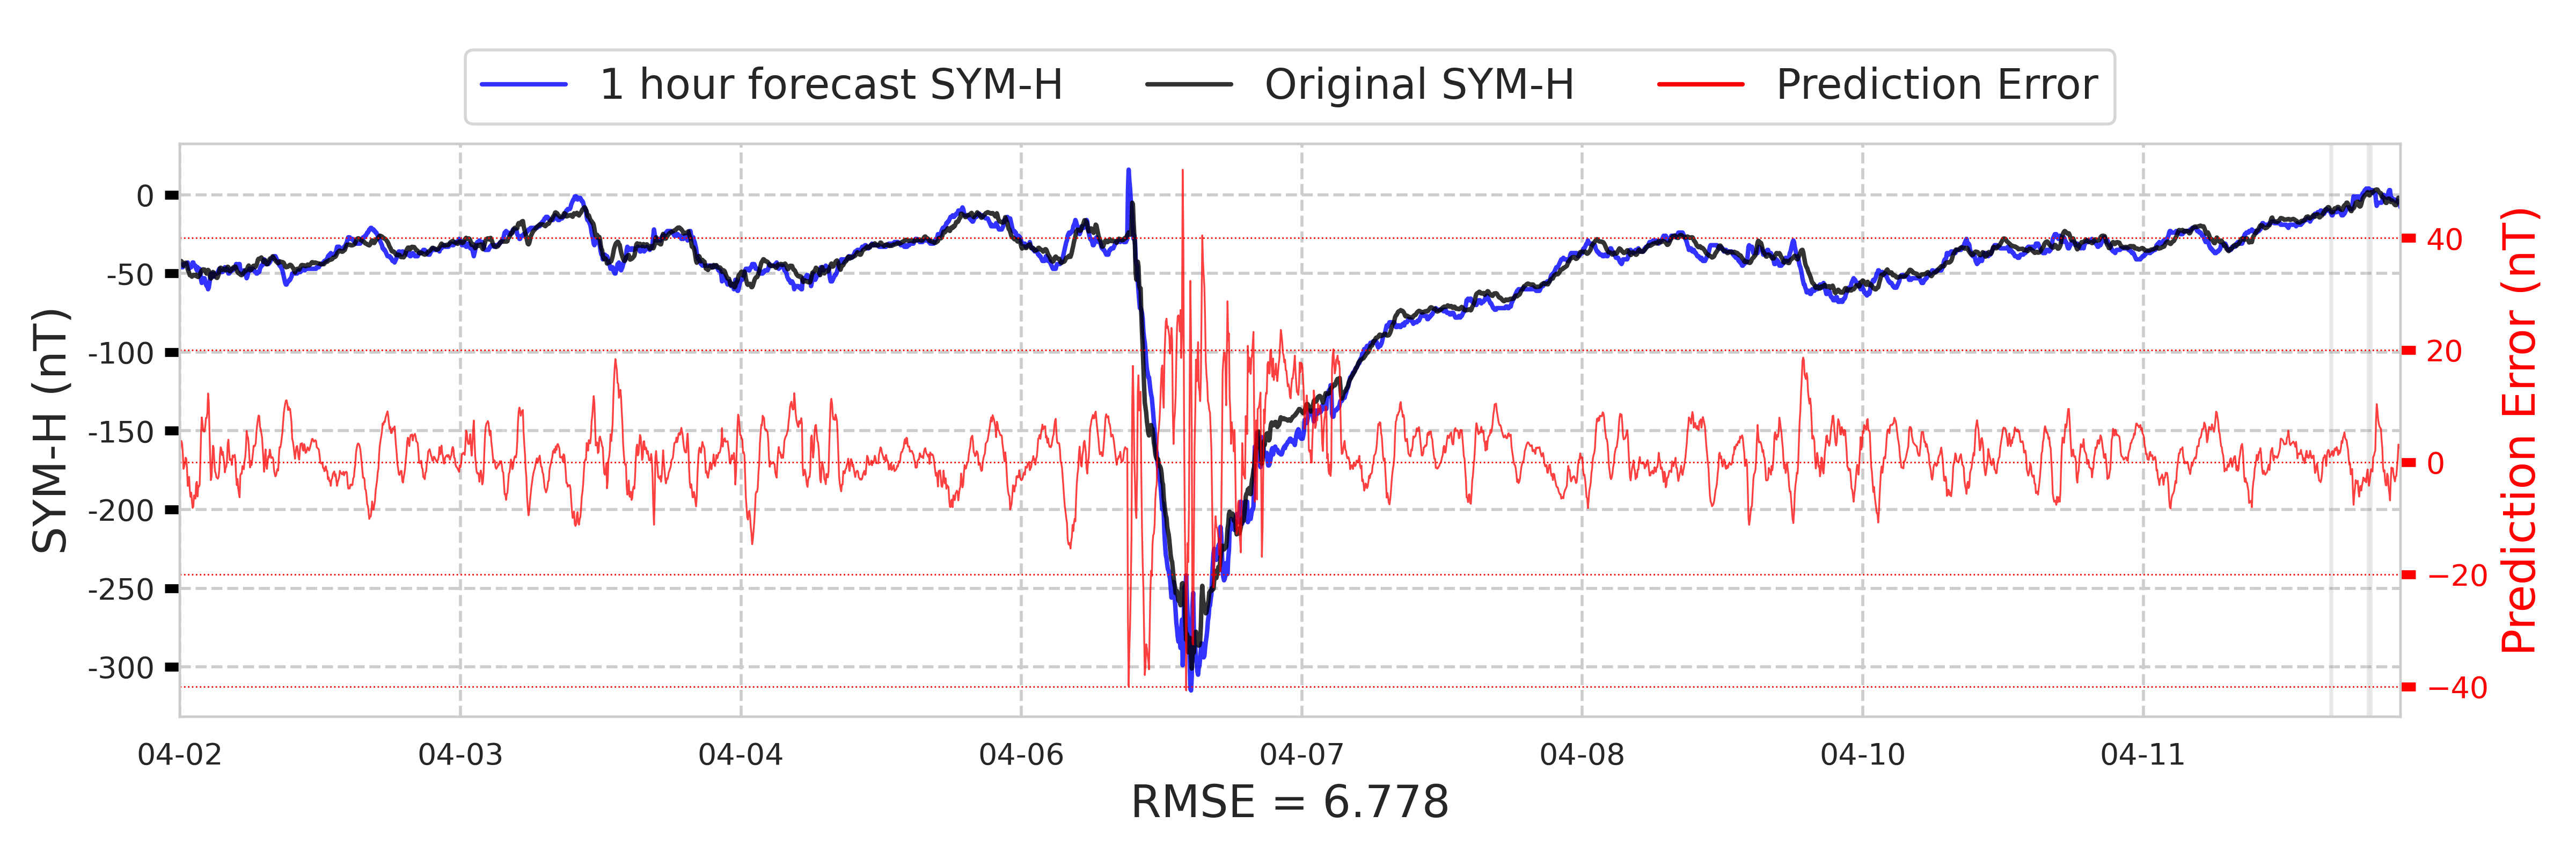
\includegraphics[width=0.49\linewidth]{paper_plots_shade/1h_swepam_rt/1h_swepam_rt_storm_31.png}
&
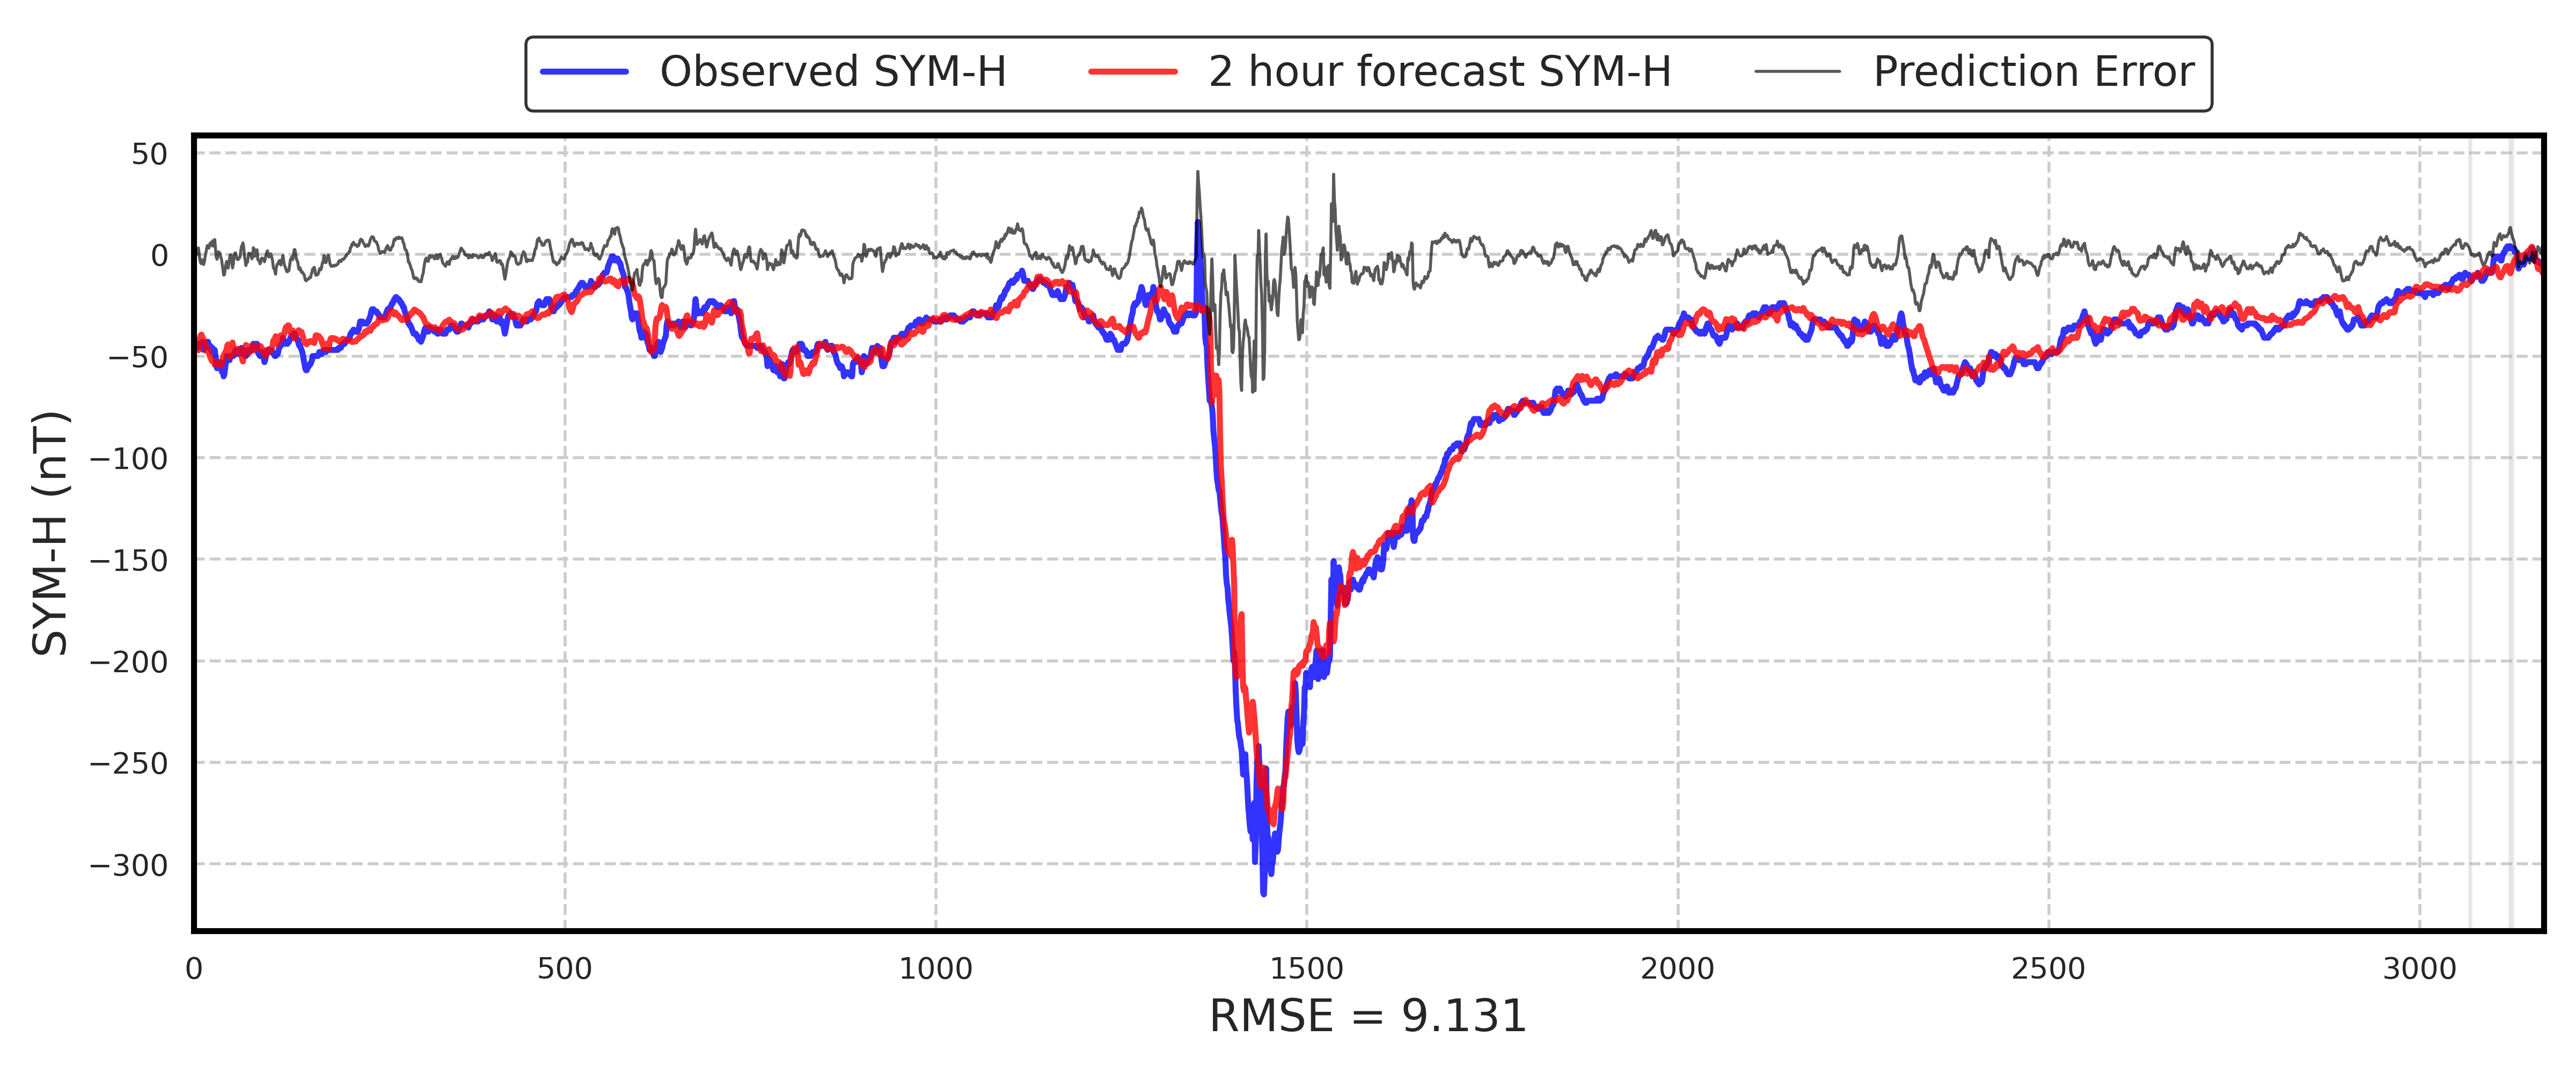
\includegraphics[width=0.49\linewidth]{paper_plots_shade/2h_swepam_rt/2h_swepam_rt_storm_31.png}
\\
\shortstack{1h operational forecast trained\\ with SWEPAM data only} & \shortstack{2h operational forecast trained\\ with SWEPAM data only}
\vspace*{12pt}
\\
\end{tabular}
\caption{Predictions for Storm Number 31 -- April of 2000}
\label{storm-31}
\end{table}



% Figure for storm 32
\begin{table}
\centering
\begin{tabular}{cc}
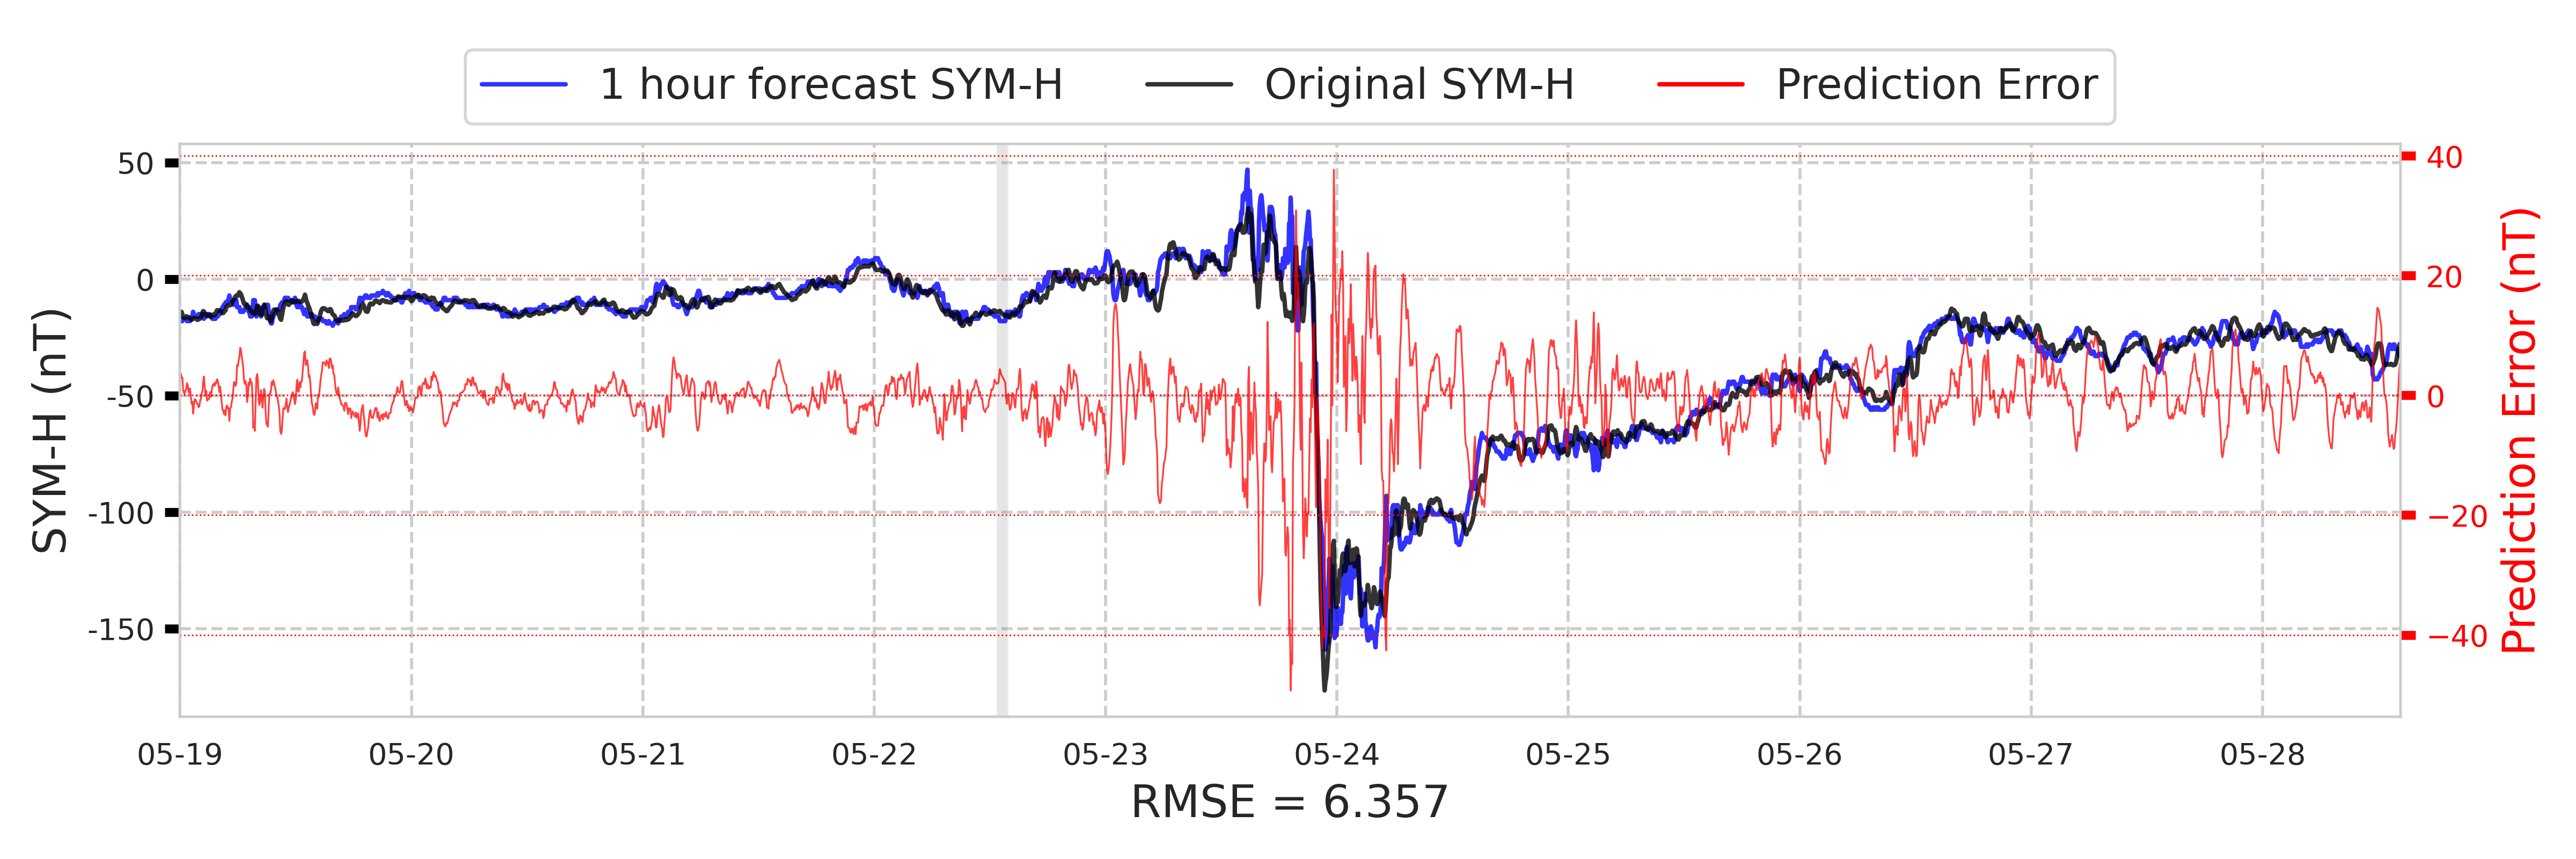
\includegraphics[width=0.49\linewidth]{paper_plots_shade/1h_swics/1h_swics_storm_32.png}
&
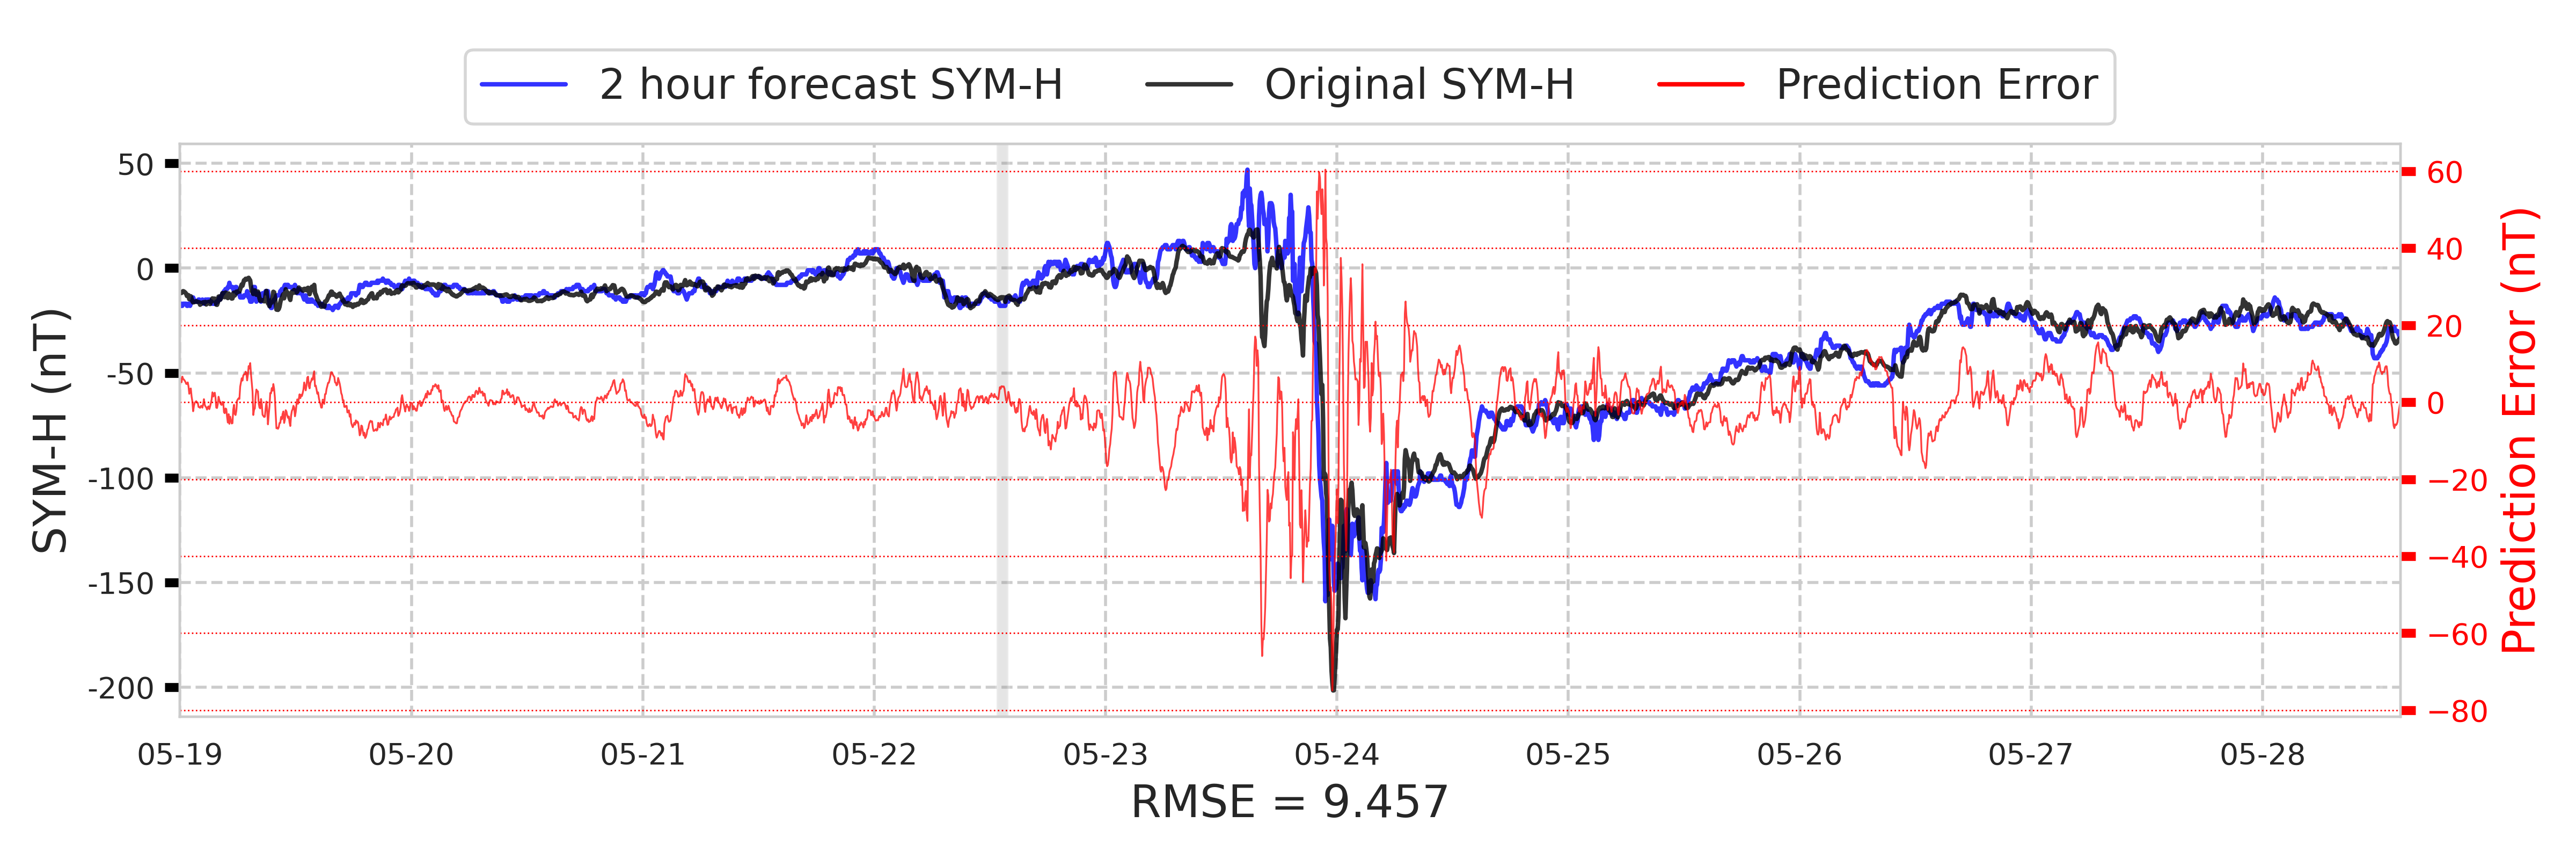
\includegraphics[width=0.49\linewidth]{paper_plots_shade/2h_swics/2h_swics_storm_32.png}
\\
\shortstack{1h forecast using SWICS\\ in laboratory conditions} & \shortstack{2h forecast using SWICS\\ in laboratory conditions}
\vspace*{12pt}
\\
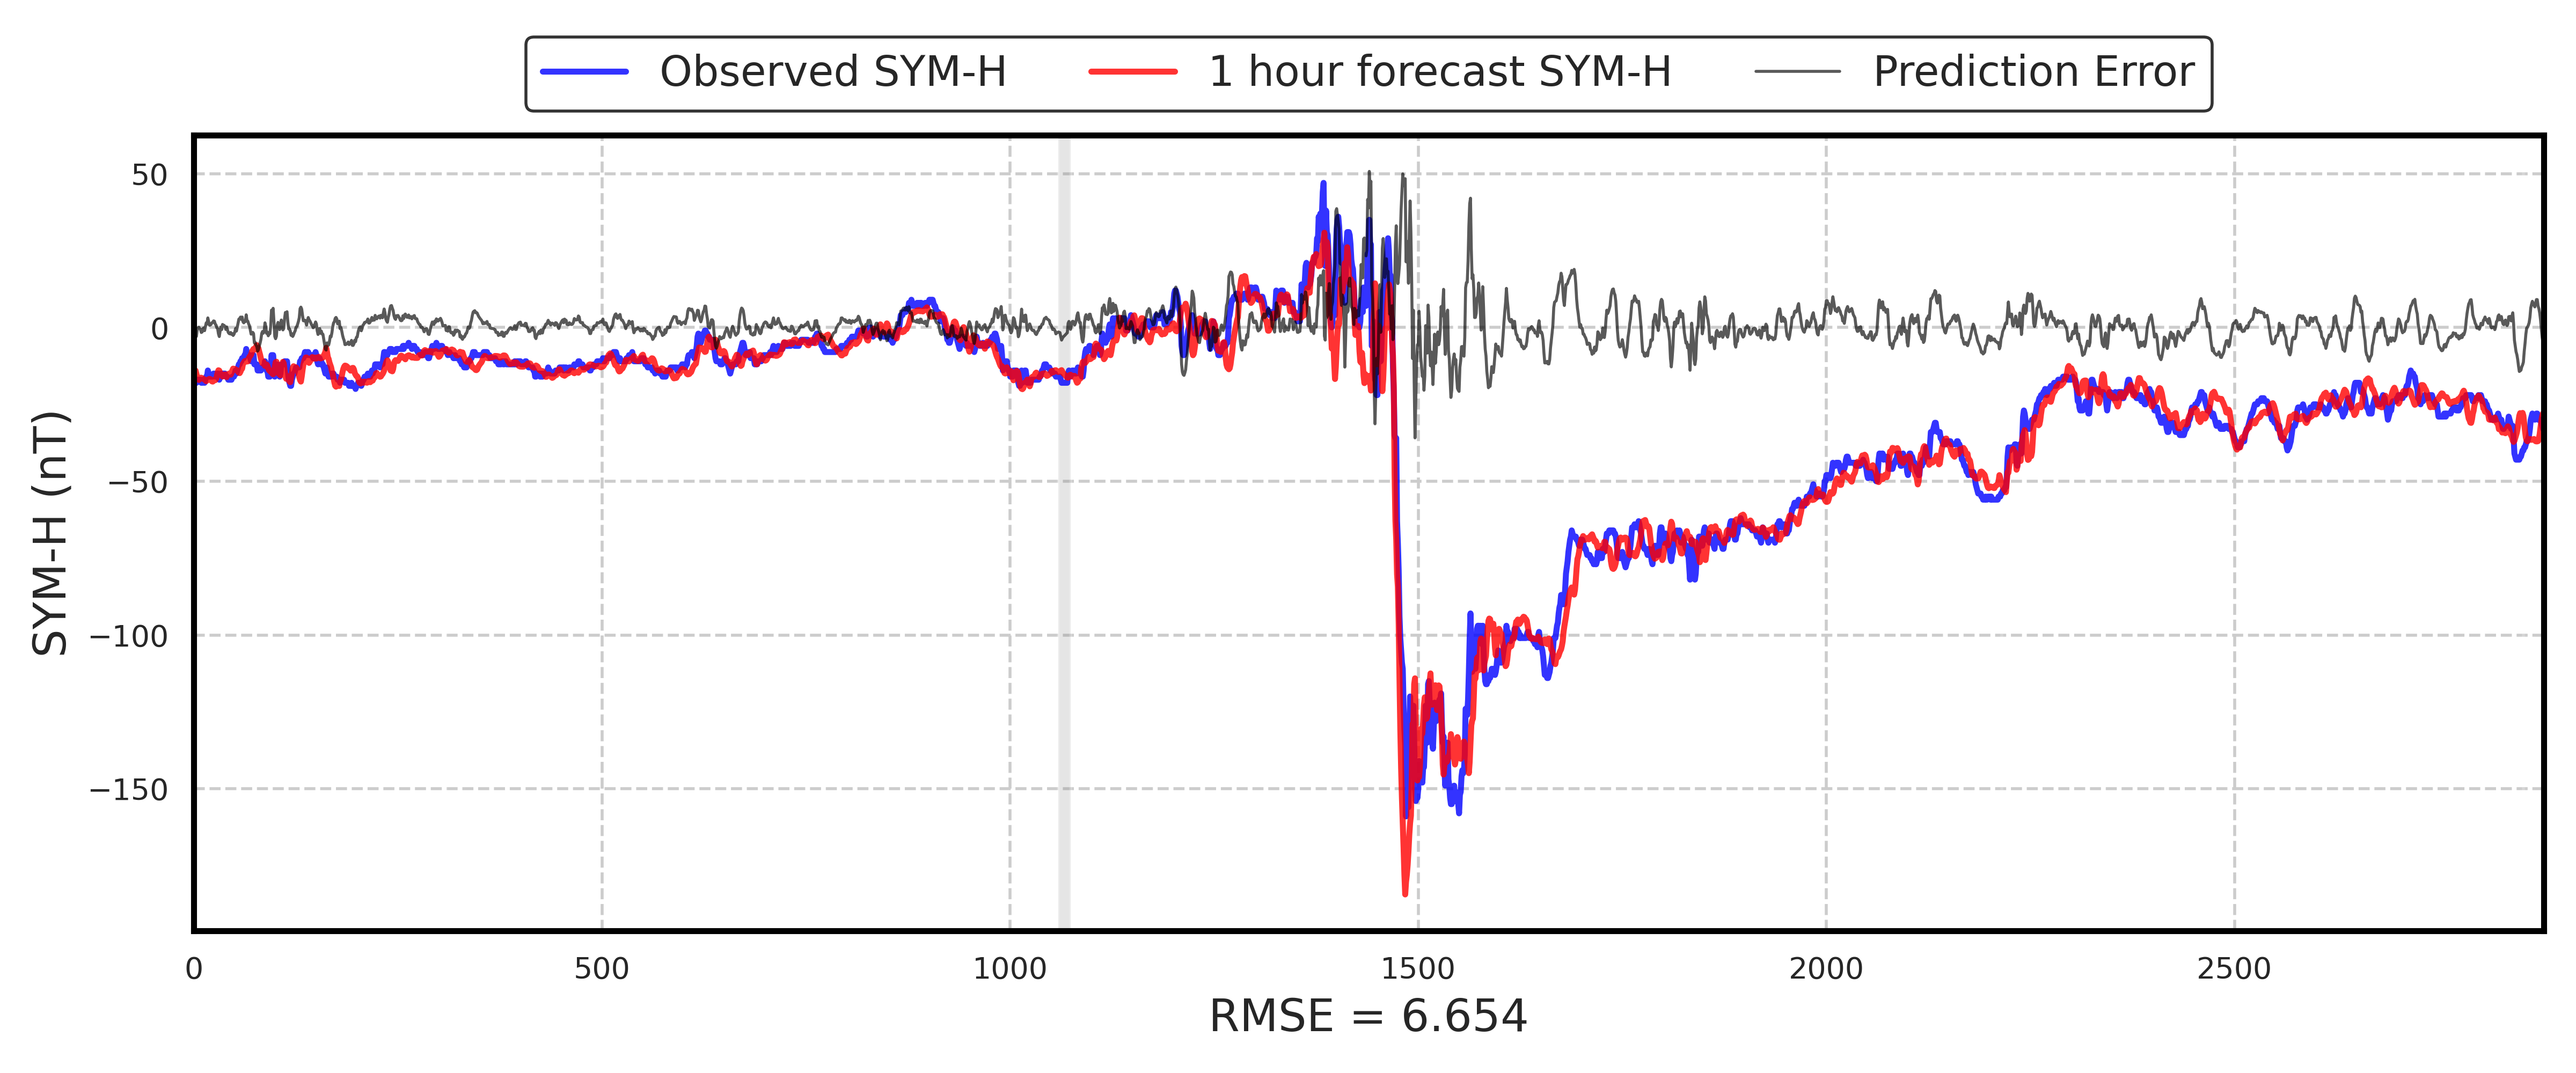
\includegraphics[width=0.49\linewidth]{paper_plots_shade/1h_swics_rt/1h_swics_rt_storm_32.png}
&
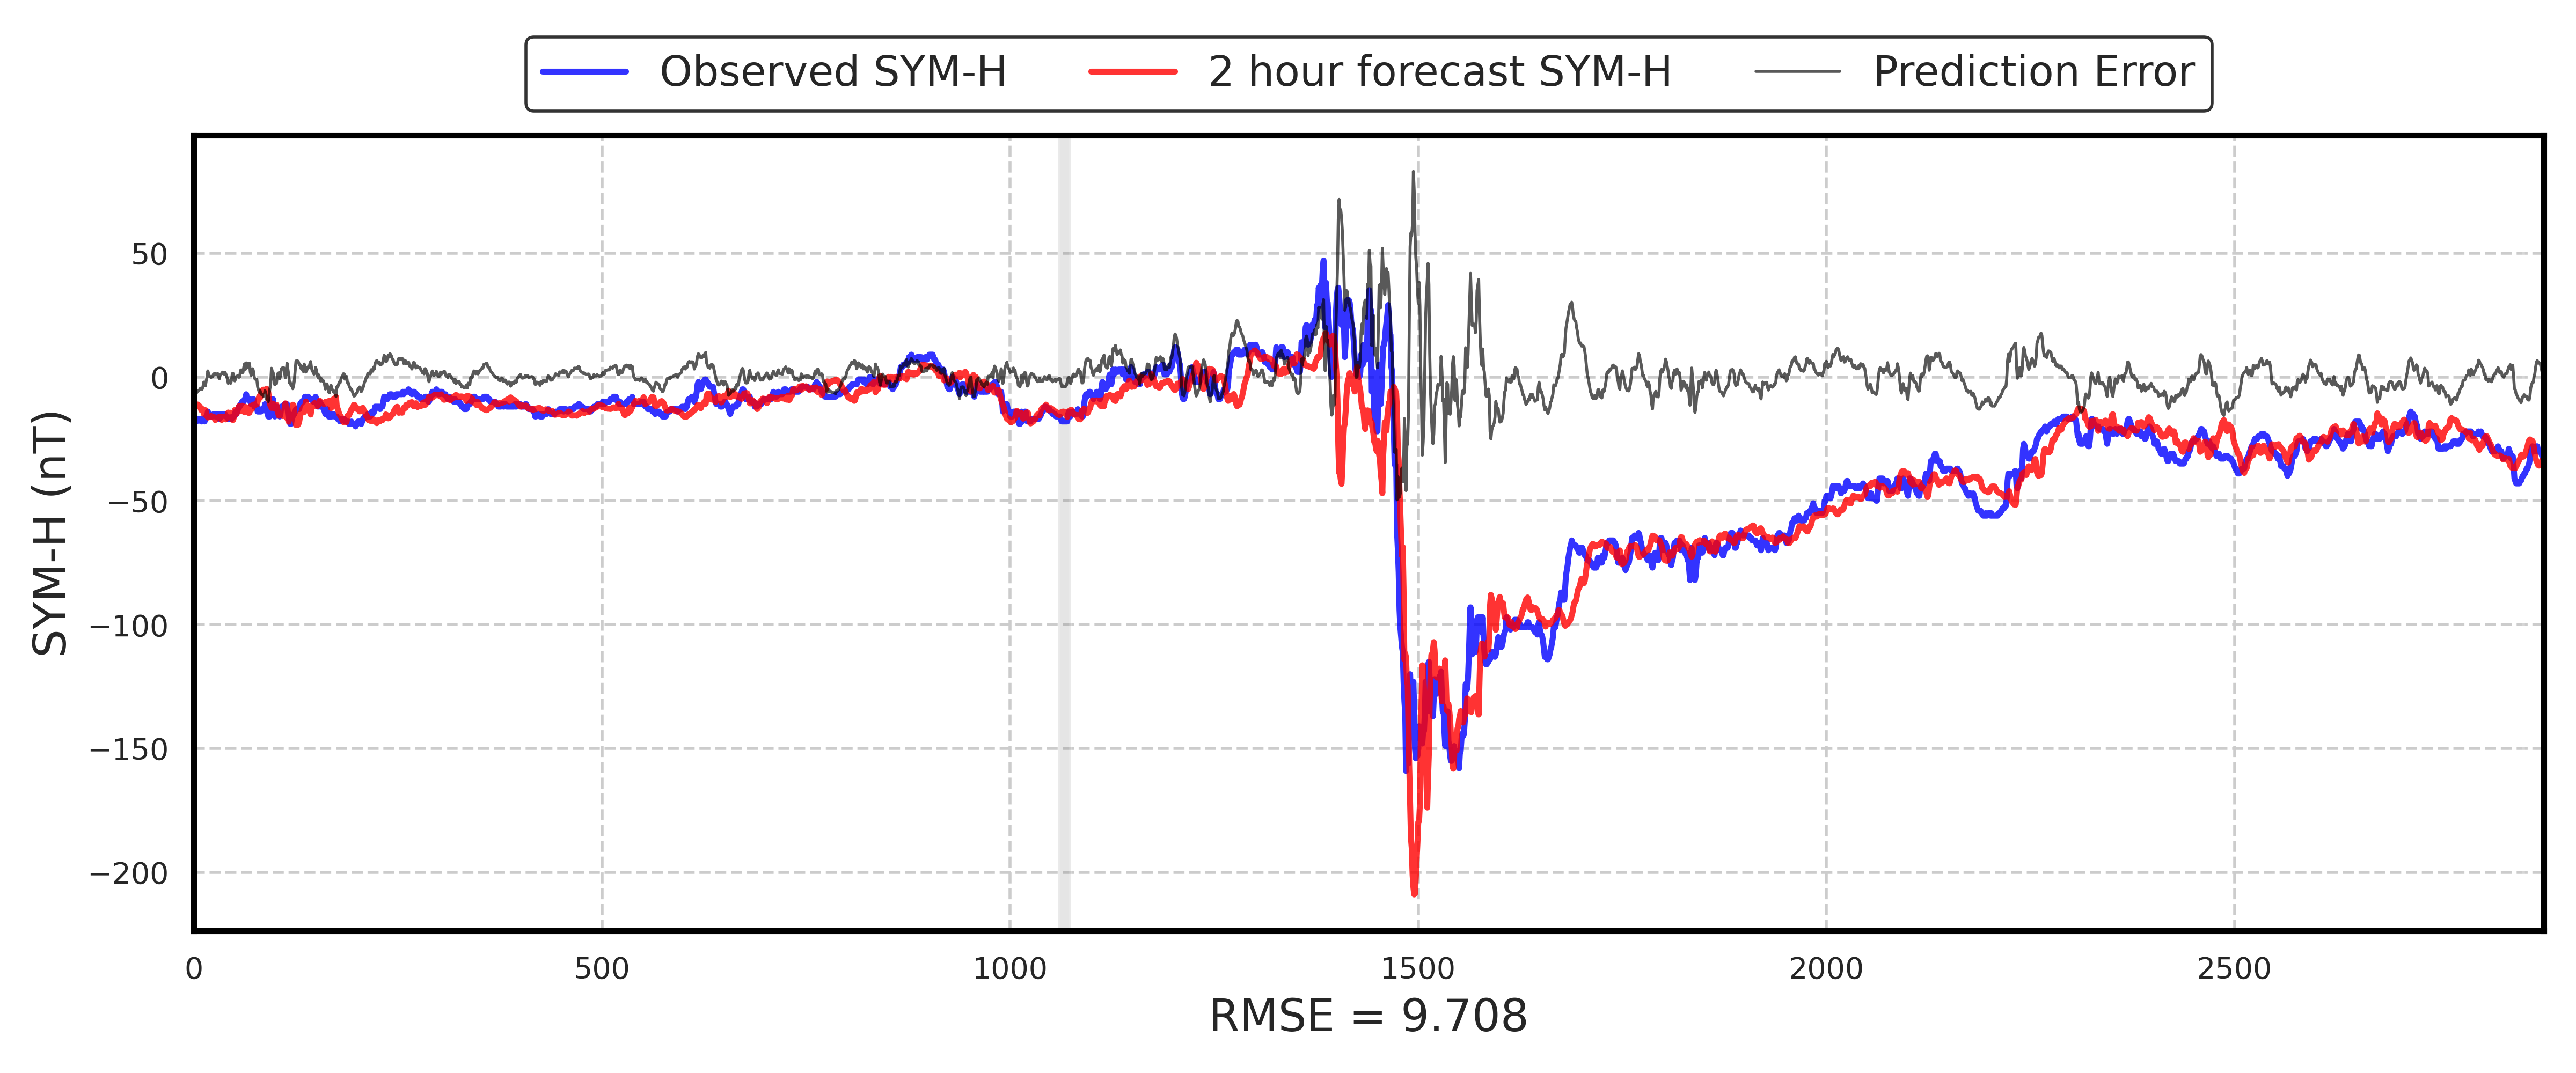
\includegraphics[width=0.49\linewidth]{paper_plots_shade/2h_swics_rt/2h_swics_rt_storm_32.png}
\\
\shortstack{1h operational forecast trained\\ with SWEPAM and SWICS data} & \shortstack{2h operational forecast trained\\ with SWEPAM and SWICS data}
\vspace*{12pt}
\\
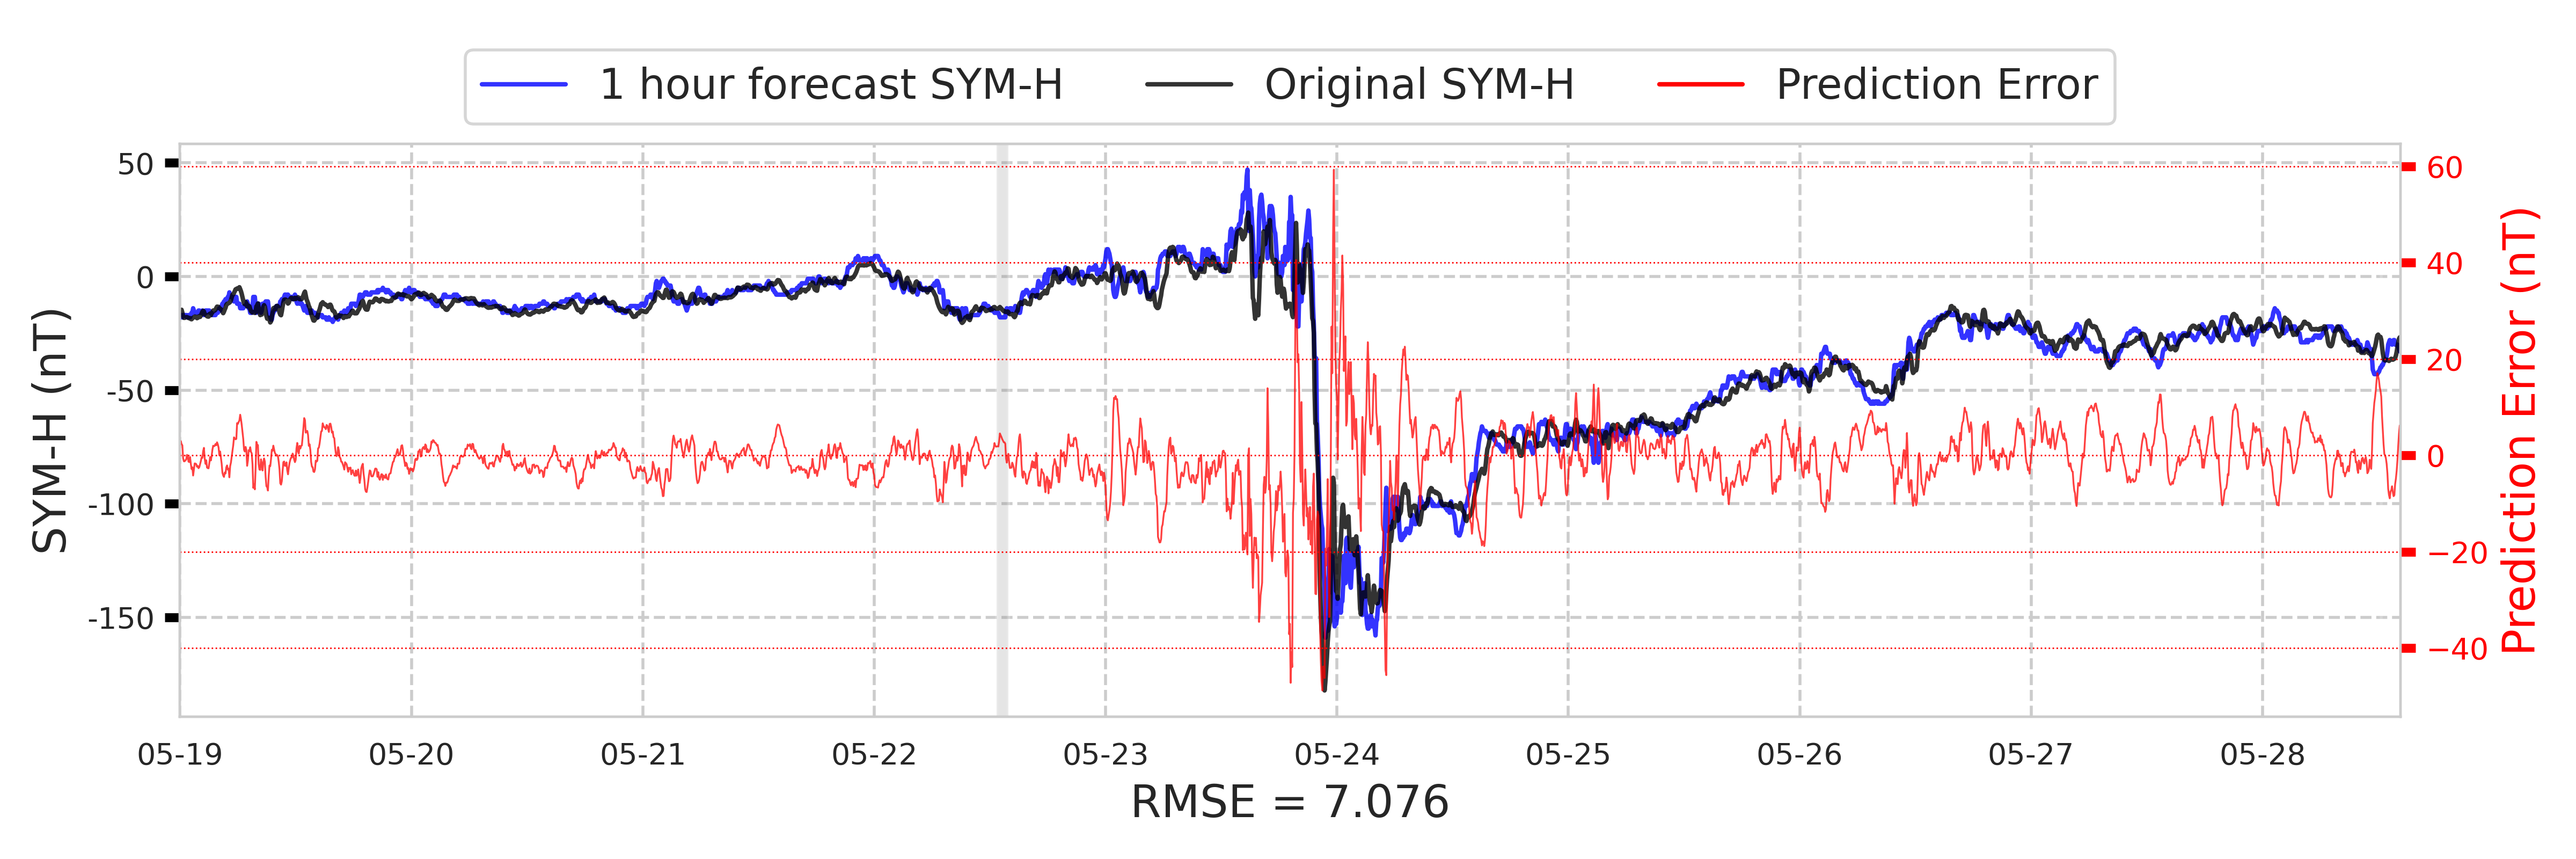
\includegraphics[width=0.49\linewidth]{paper_plots_shade/1h_swepam_rt/1h_swepam_rt_storm_32.png}
&
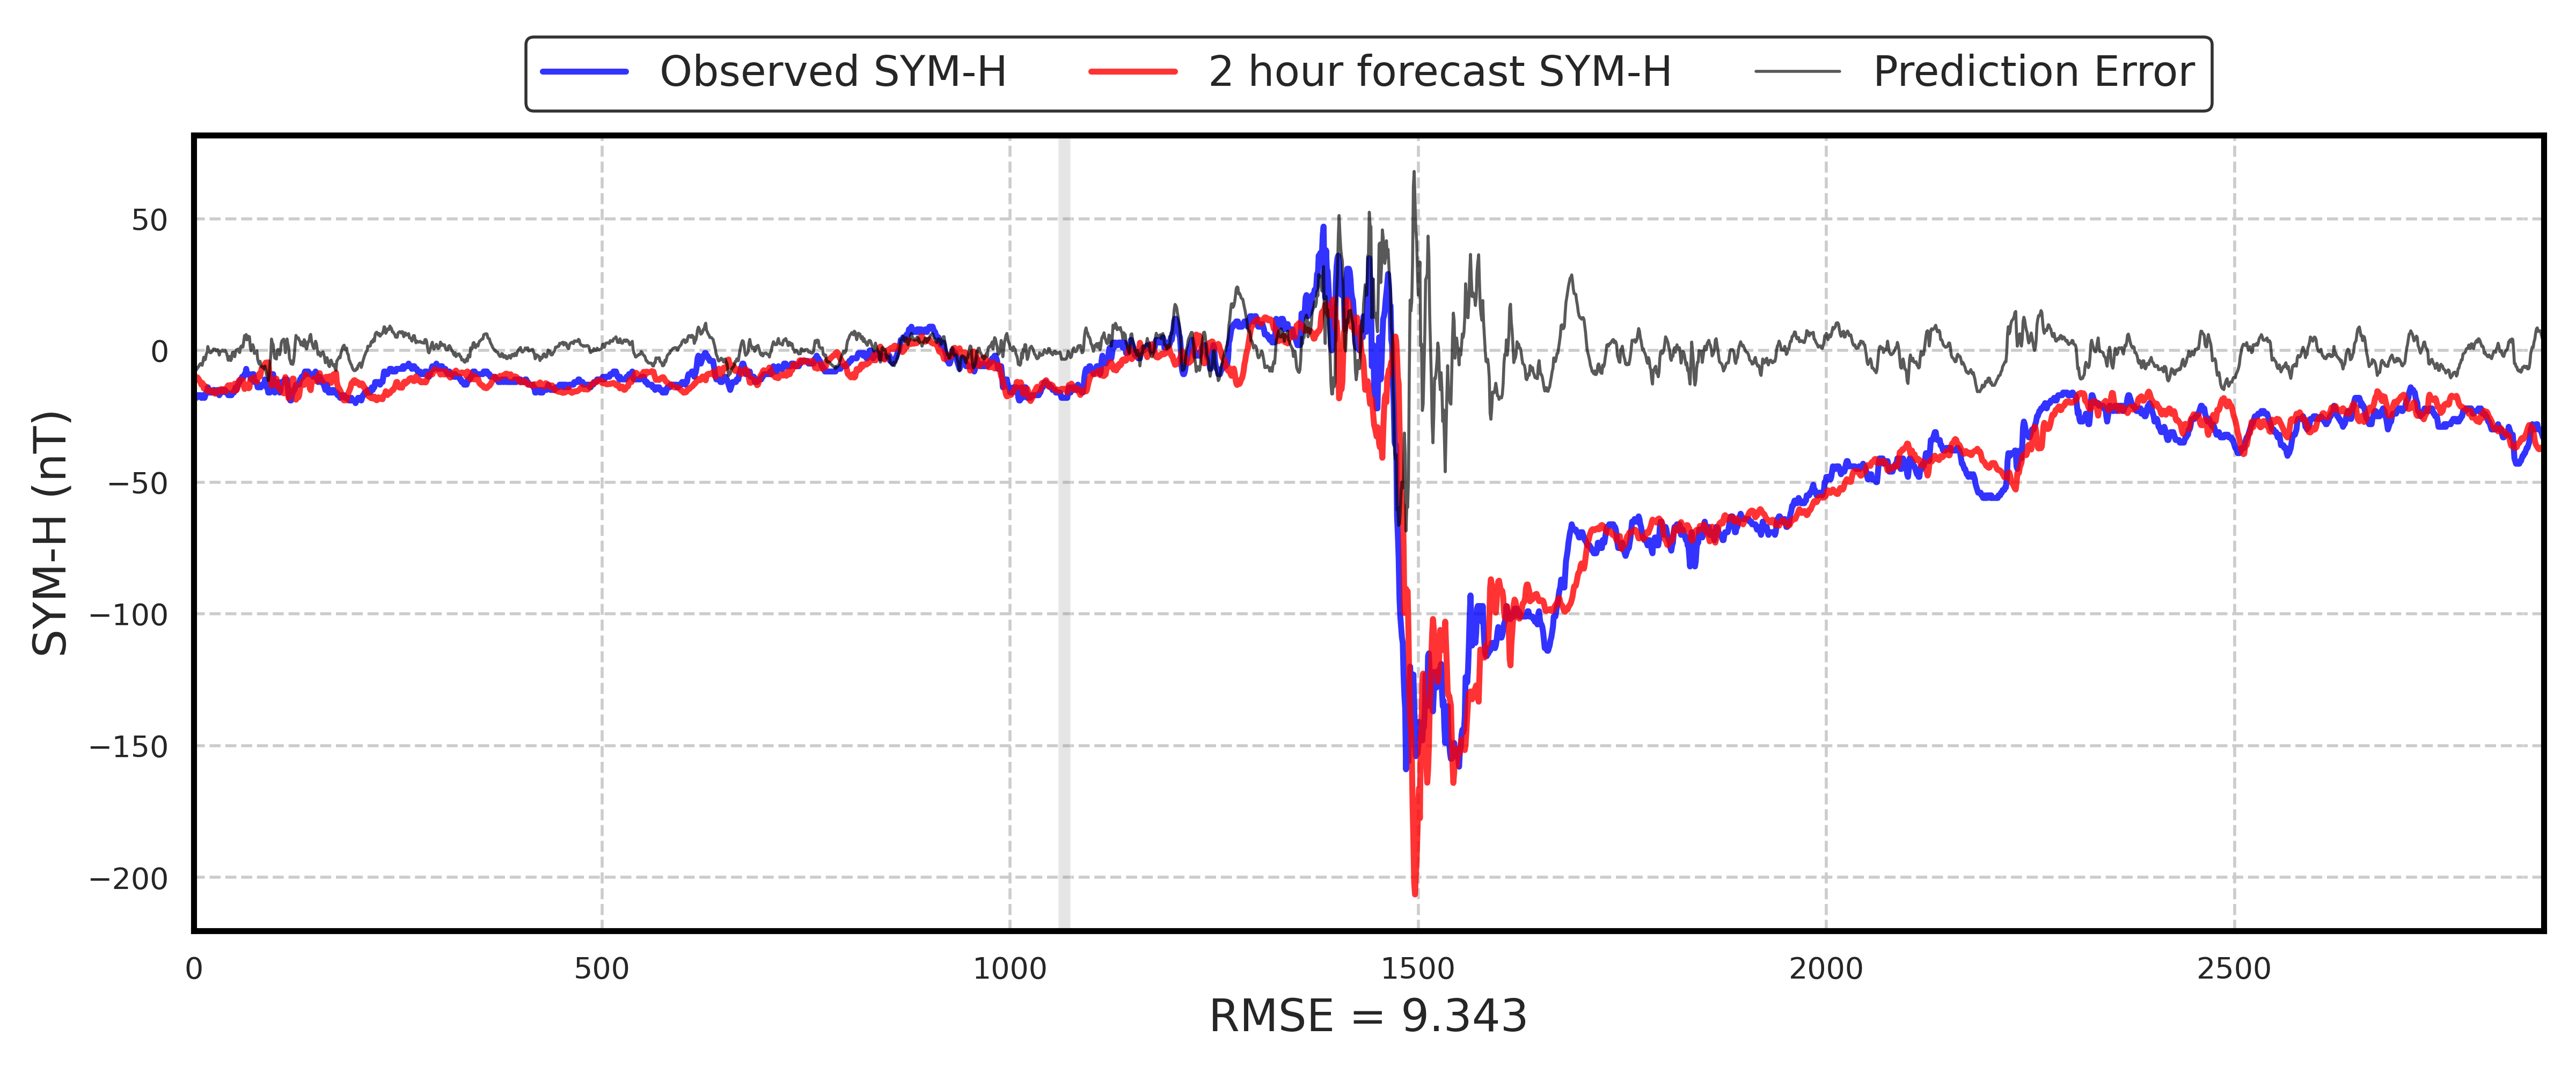
\includegraphics[width=0.49\linewidth]{paper_plots_shade/2h_swepam_rt/2h_swepam_rt_storm_32.png}
\\
\shortstack{1h operational forecast trained\\ with SWEPAM data only} & \shortstack{2h operational forecast trained\\ with SWEPAM data only}
\vspace*{12pt}
\\
\end{tabular}
\caption{Predictions for Storm Number 32 -- May of 2000}
\label{storm-32}
\end{table}



% Figure for storm 33
\begin{table}
\centering
\begin{tabular}{cc}
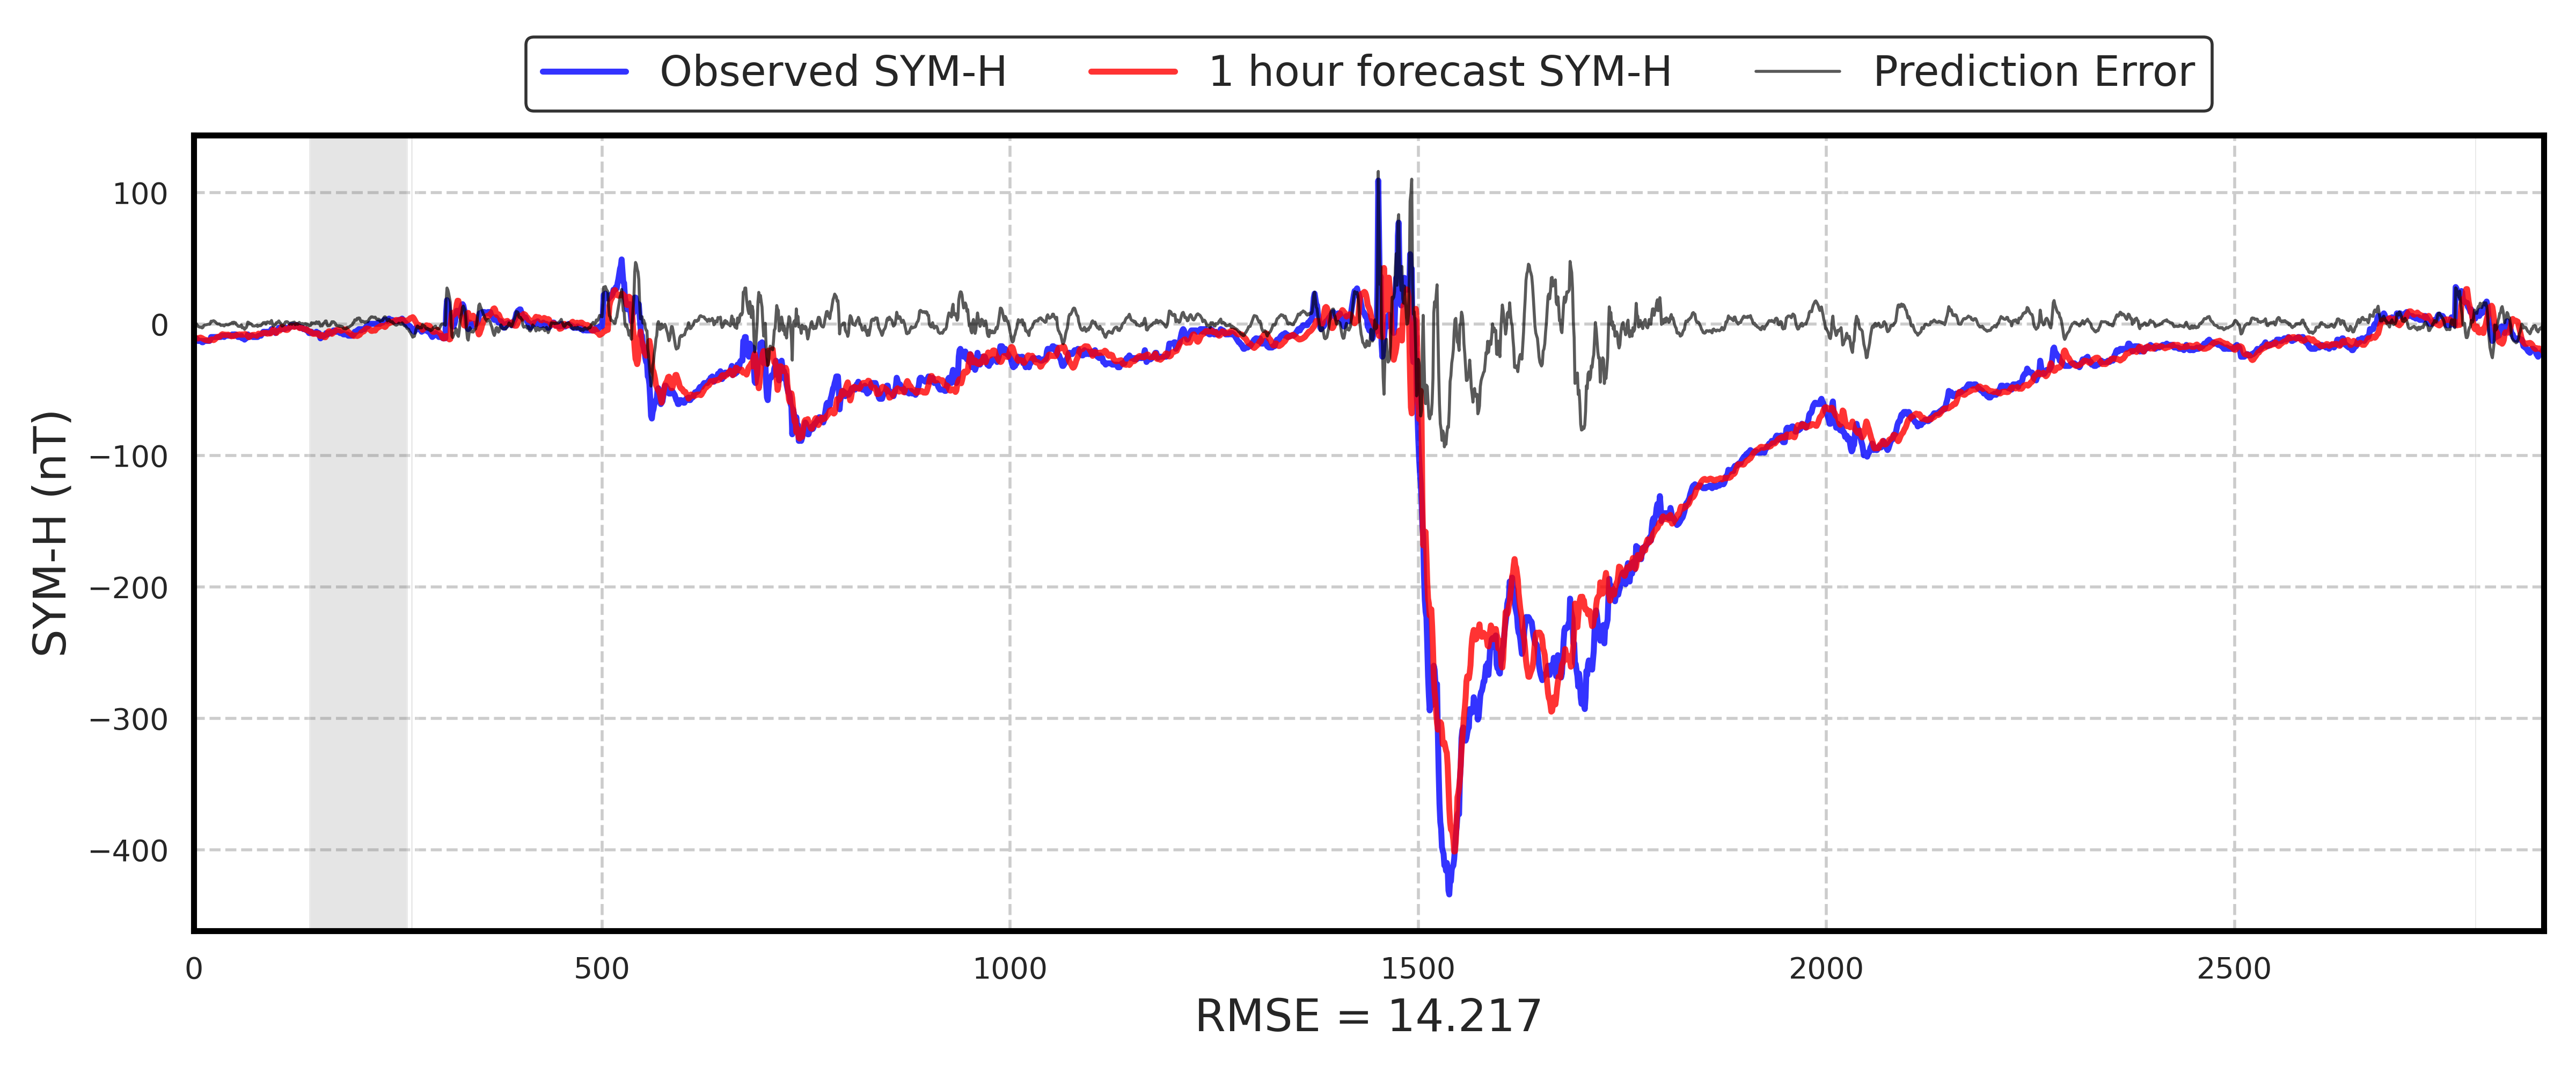
\includegraphics[width=0.49\linewidth]{paper_plots_shade/1h_swics/1h_swics_storm_33.png}
&
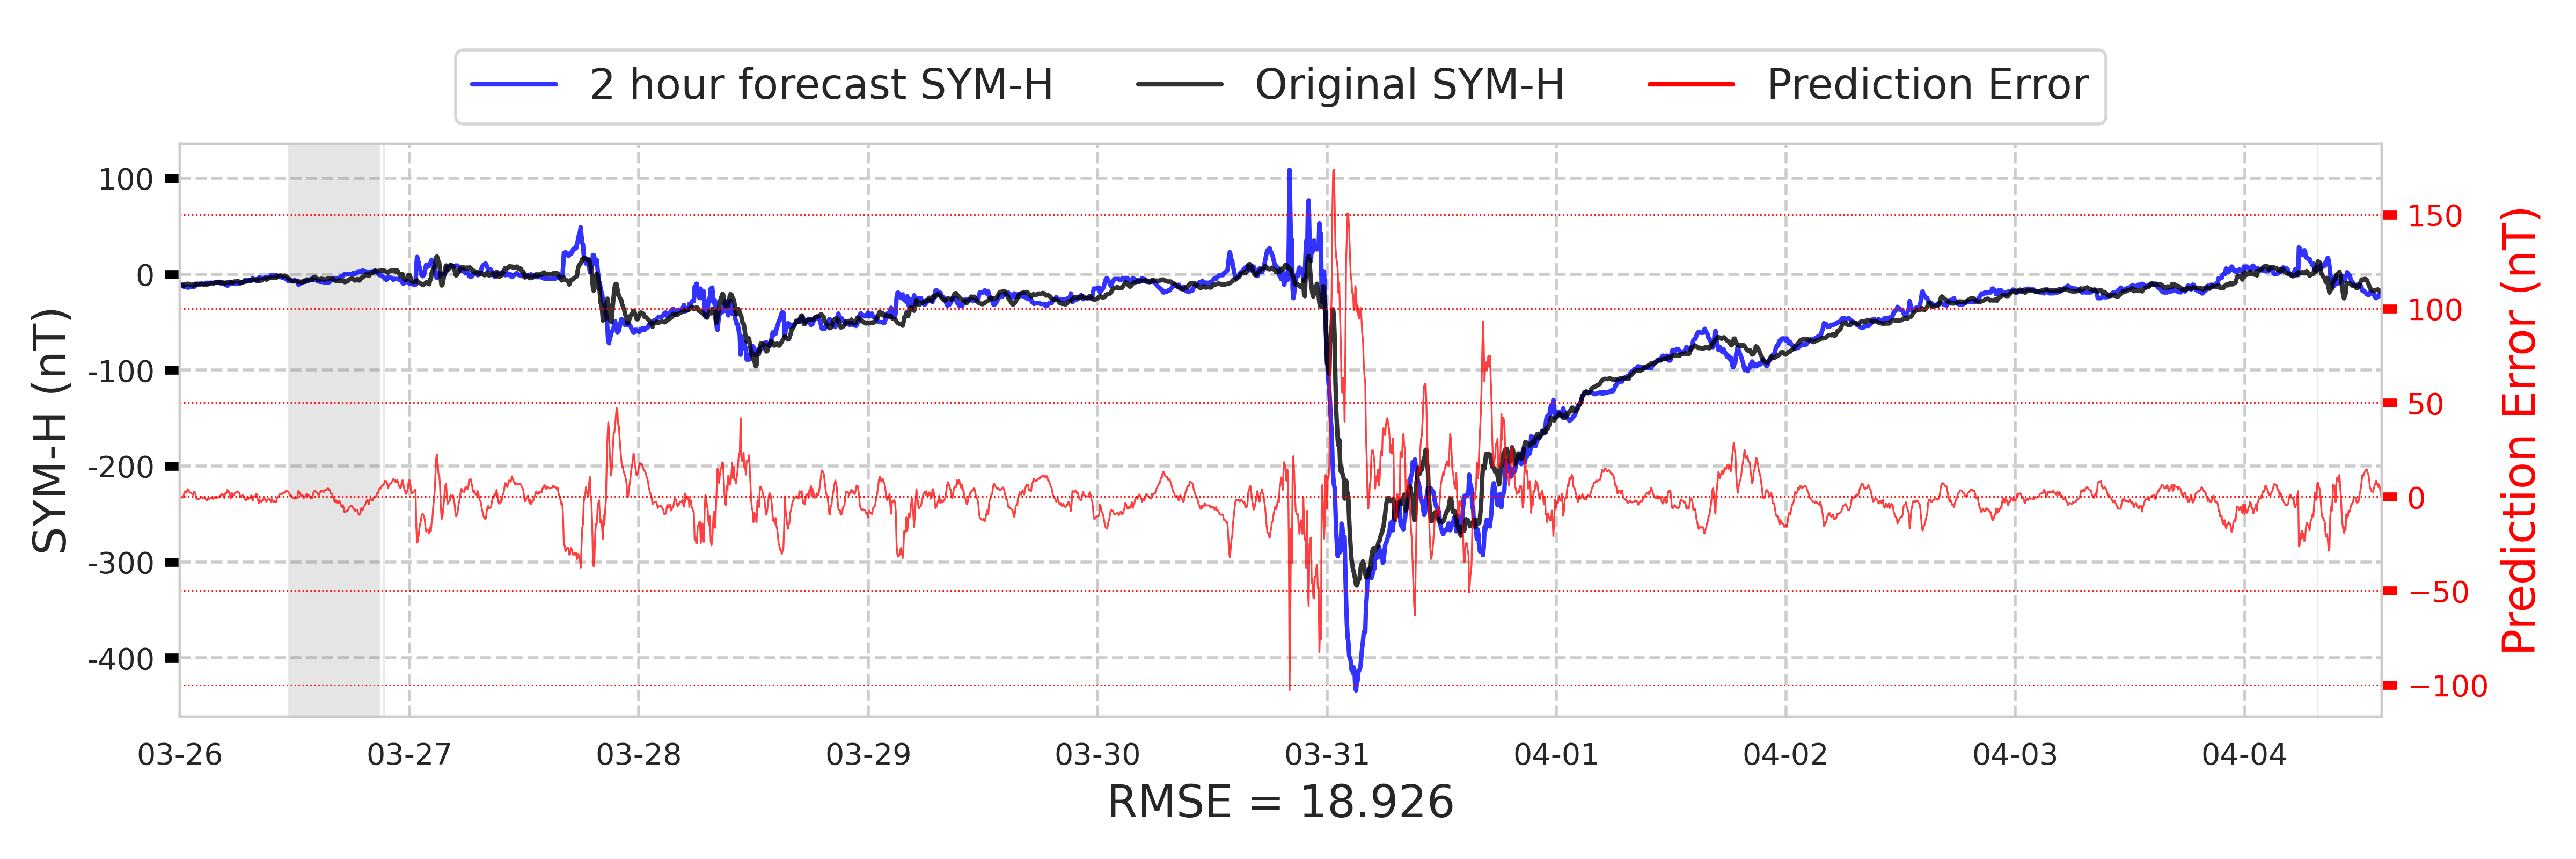
\includegraphics[width=0.49\linewidth]{paper_plots_shade/2h_swics/2h_swics_storm_33.png}
\\
\shortstack{1h forecast using SWICS\\ in laboratory conditions} & \shortstack{2h forecast using SWICS\\ in laboratory conditions}
\vspace*{12pt}
\\
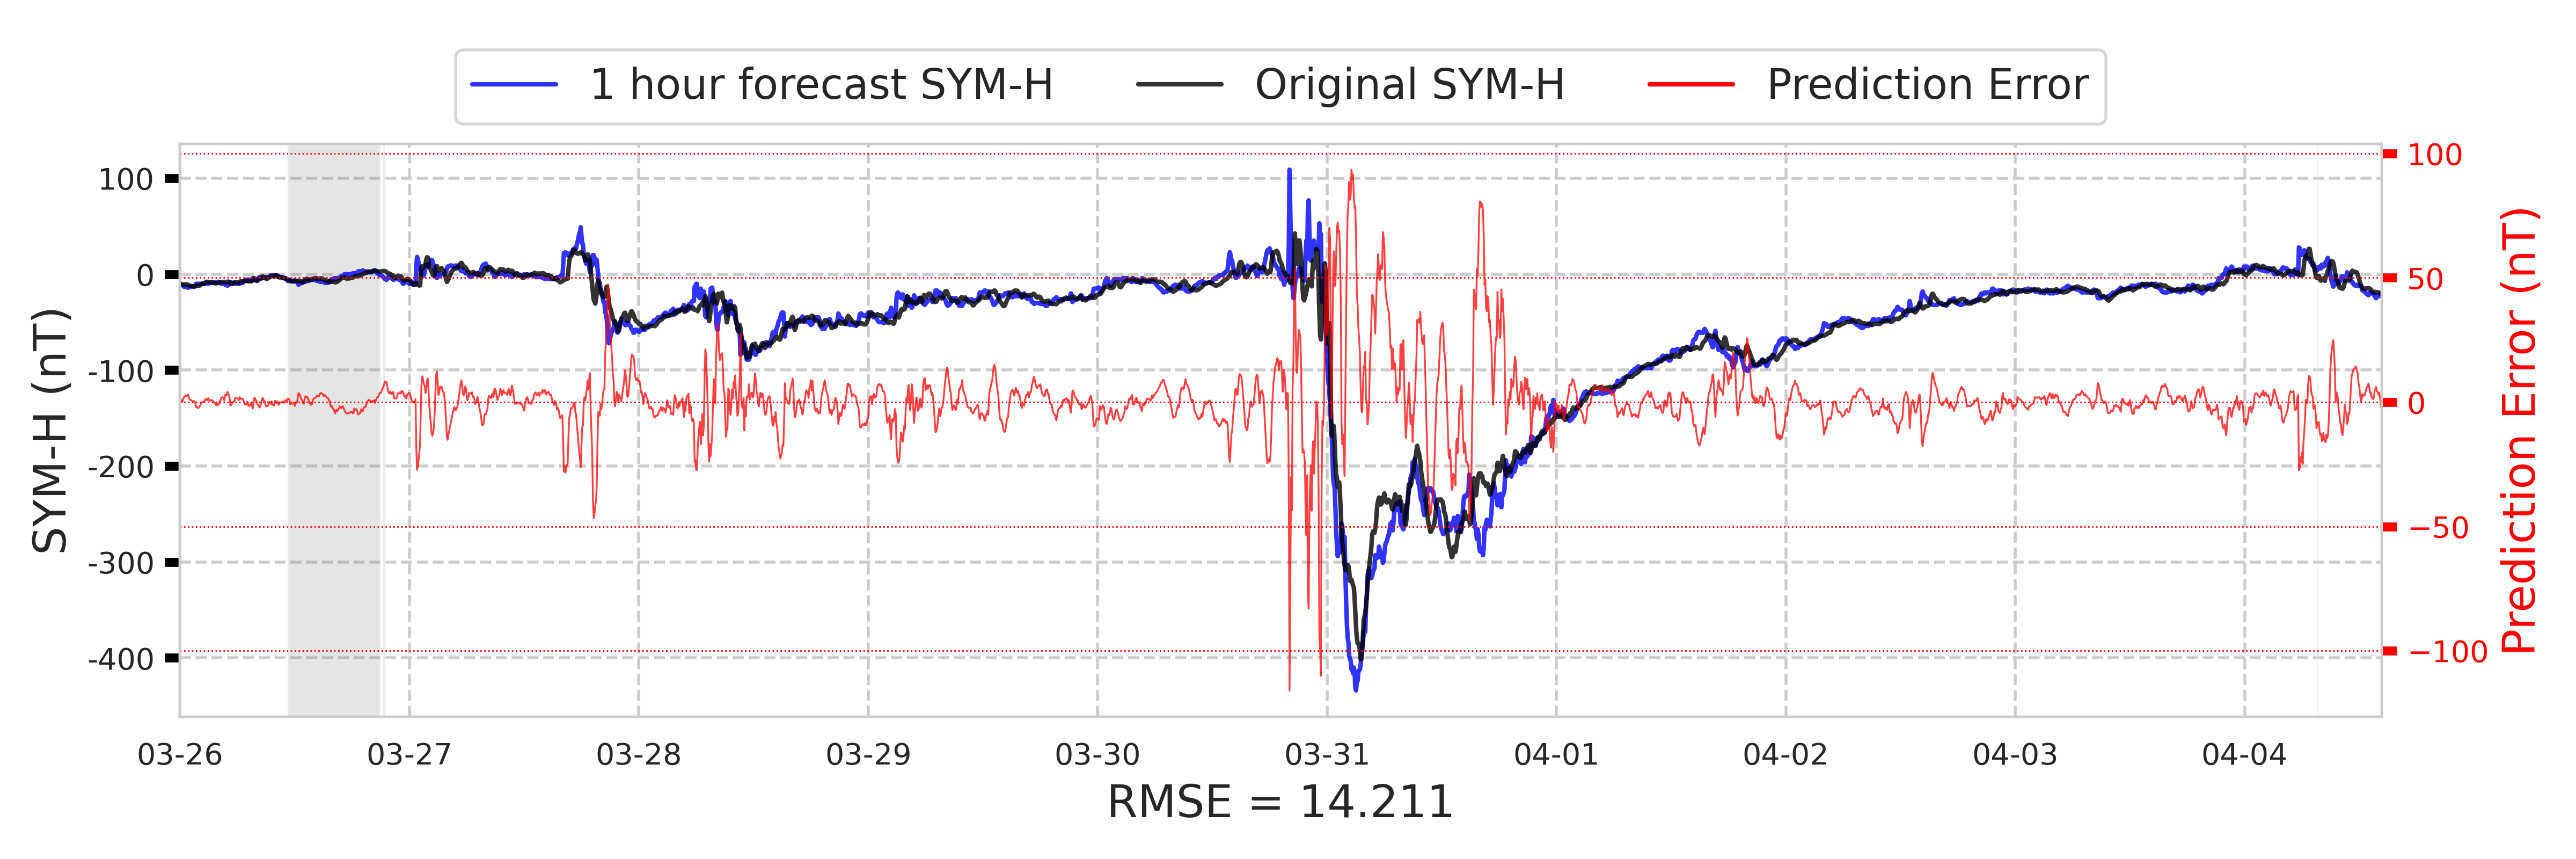
\includegraphics[width=0.49\linewidth]{paper_plots_shade/1h_swics_rt/1h_swics_rt_storm_33.png}
&
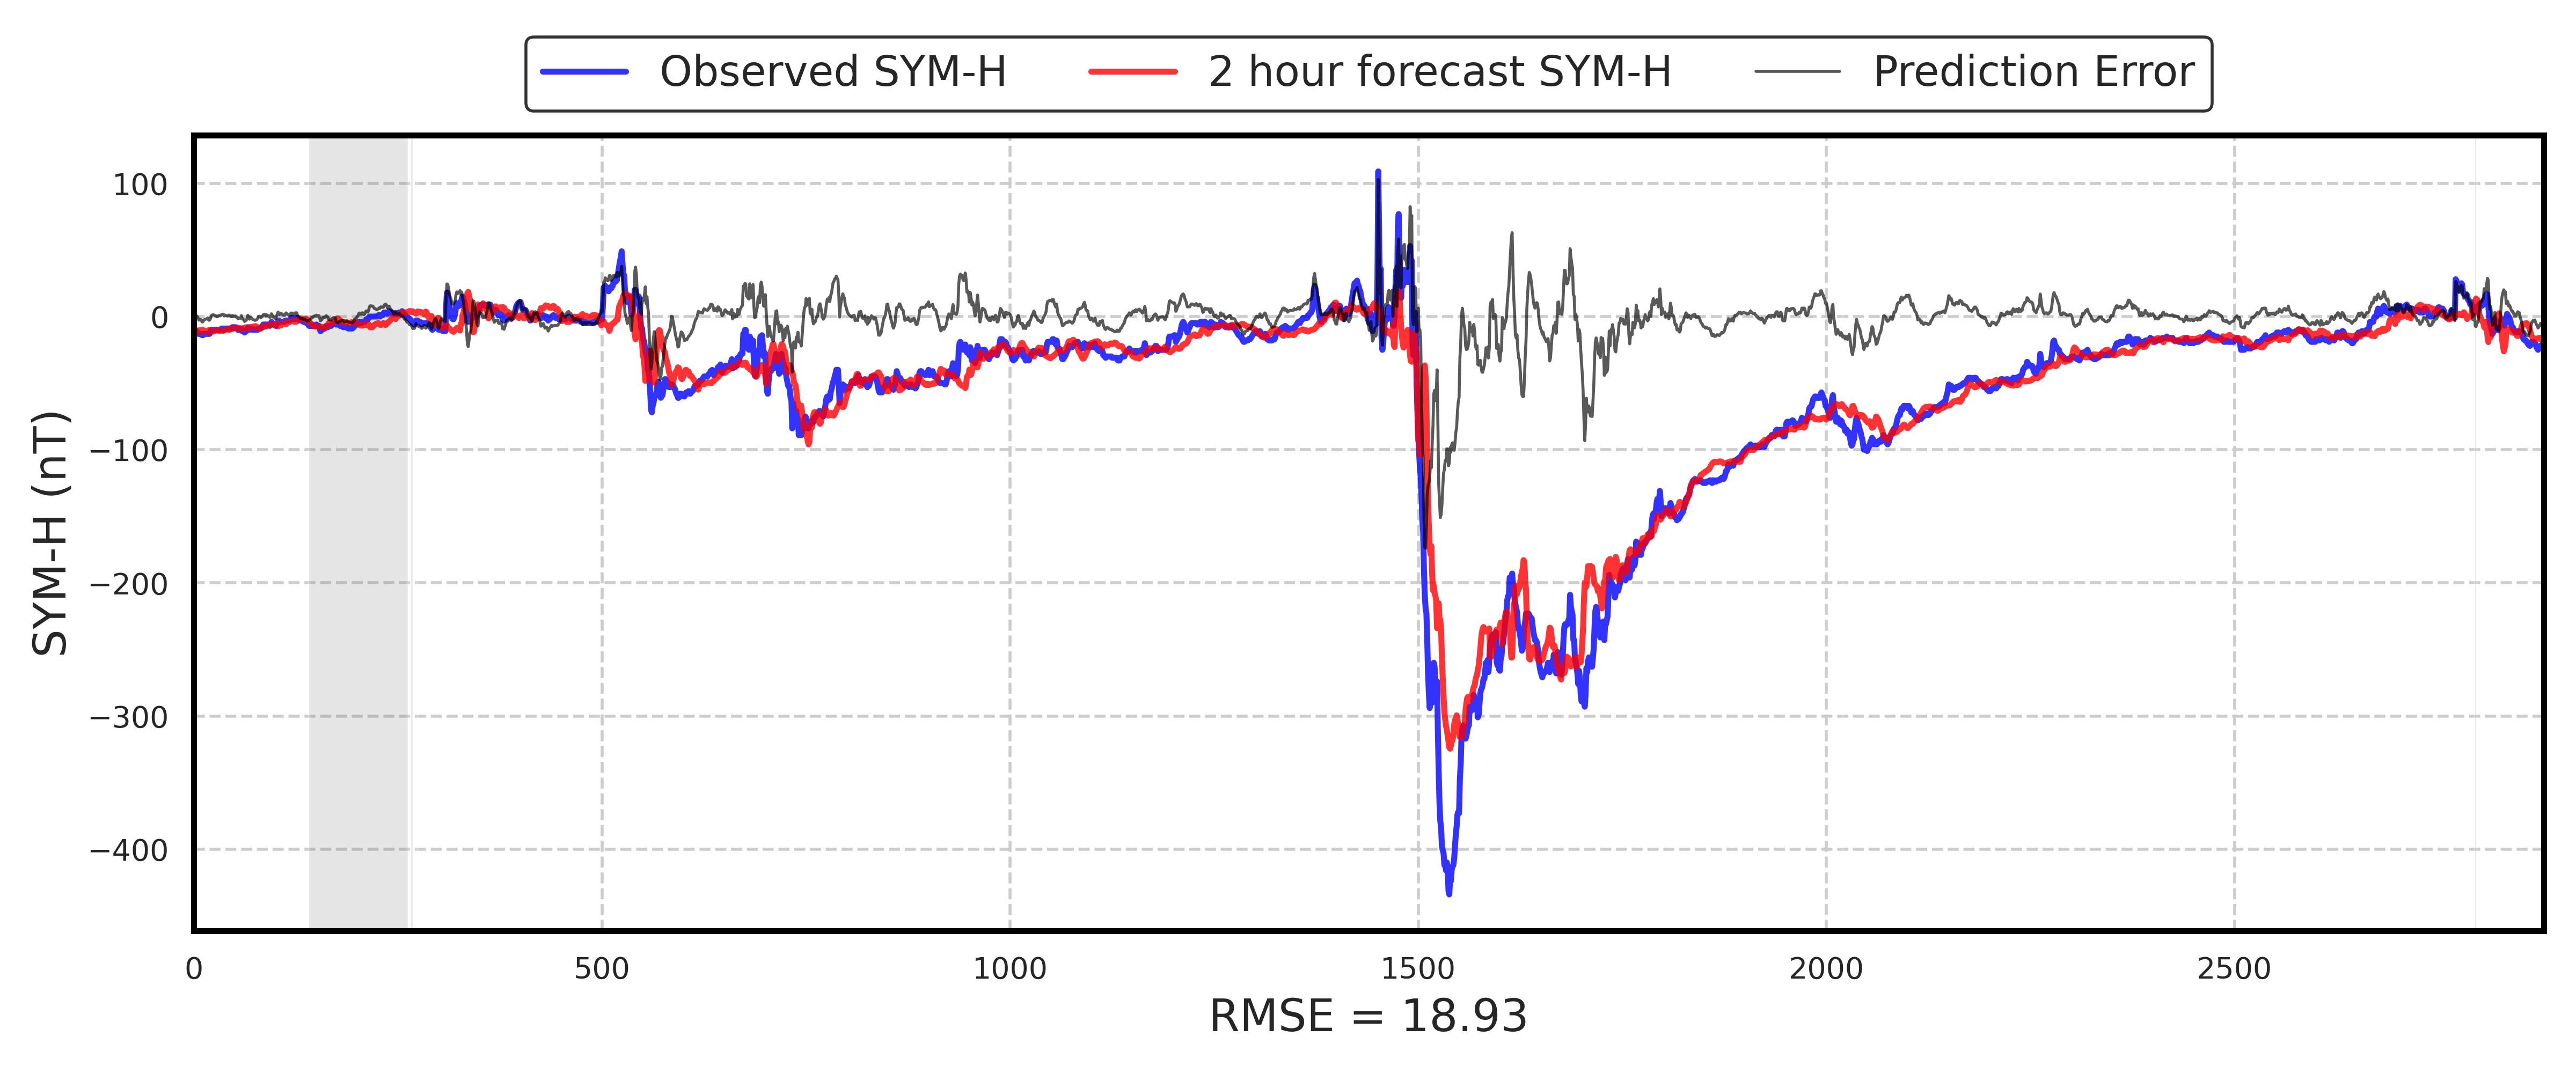
\includegraphics[width=0.49\linewidth]{paper_plots_shade/2h_swics_rt/2h_swics_rt_storm_33.png}
\\
\shortstack{1h operational forecast trained\\ with SWEPAM and SWICS data} & \shortstack{2h operational forecast trained\\ with SWEPAM and SWICS data}
\vspace*{12pt}
\\
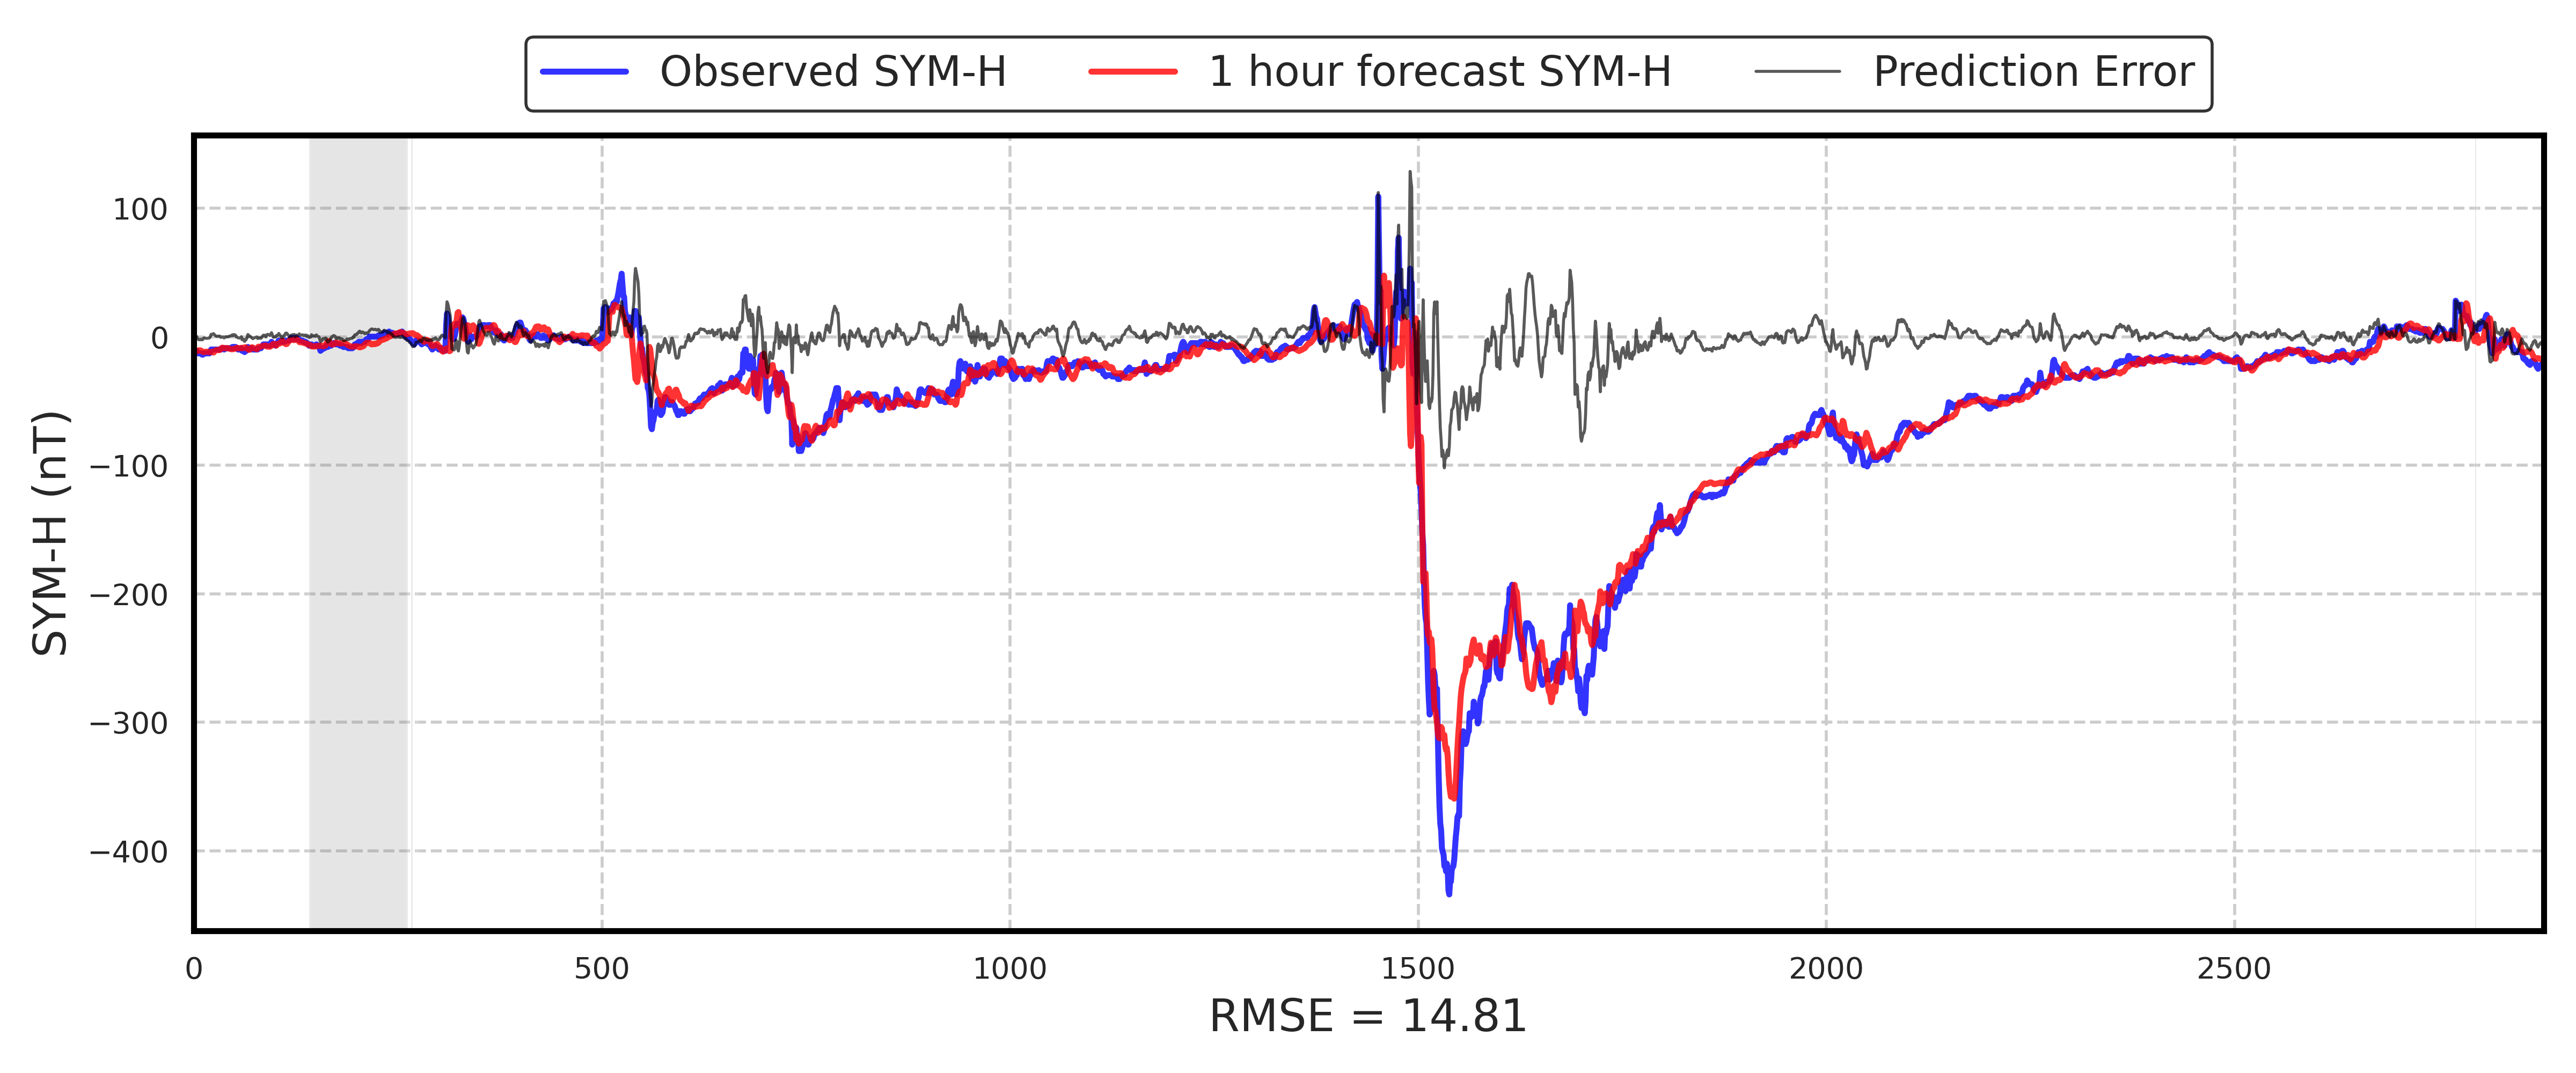
\includegraphics[width=0.49\linewidth]{paper_plots_shade/1h_swepam_rt/1h_swepam_rt_storm_33.png}
&
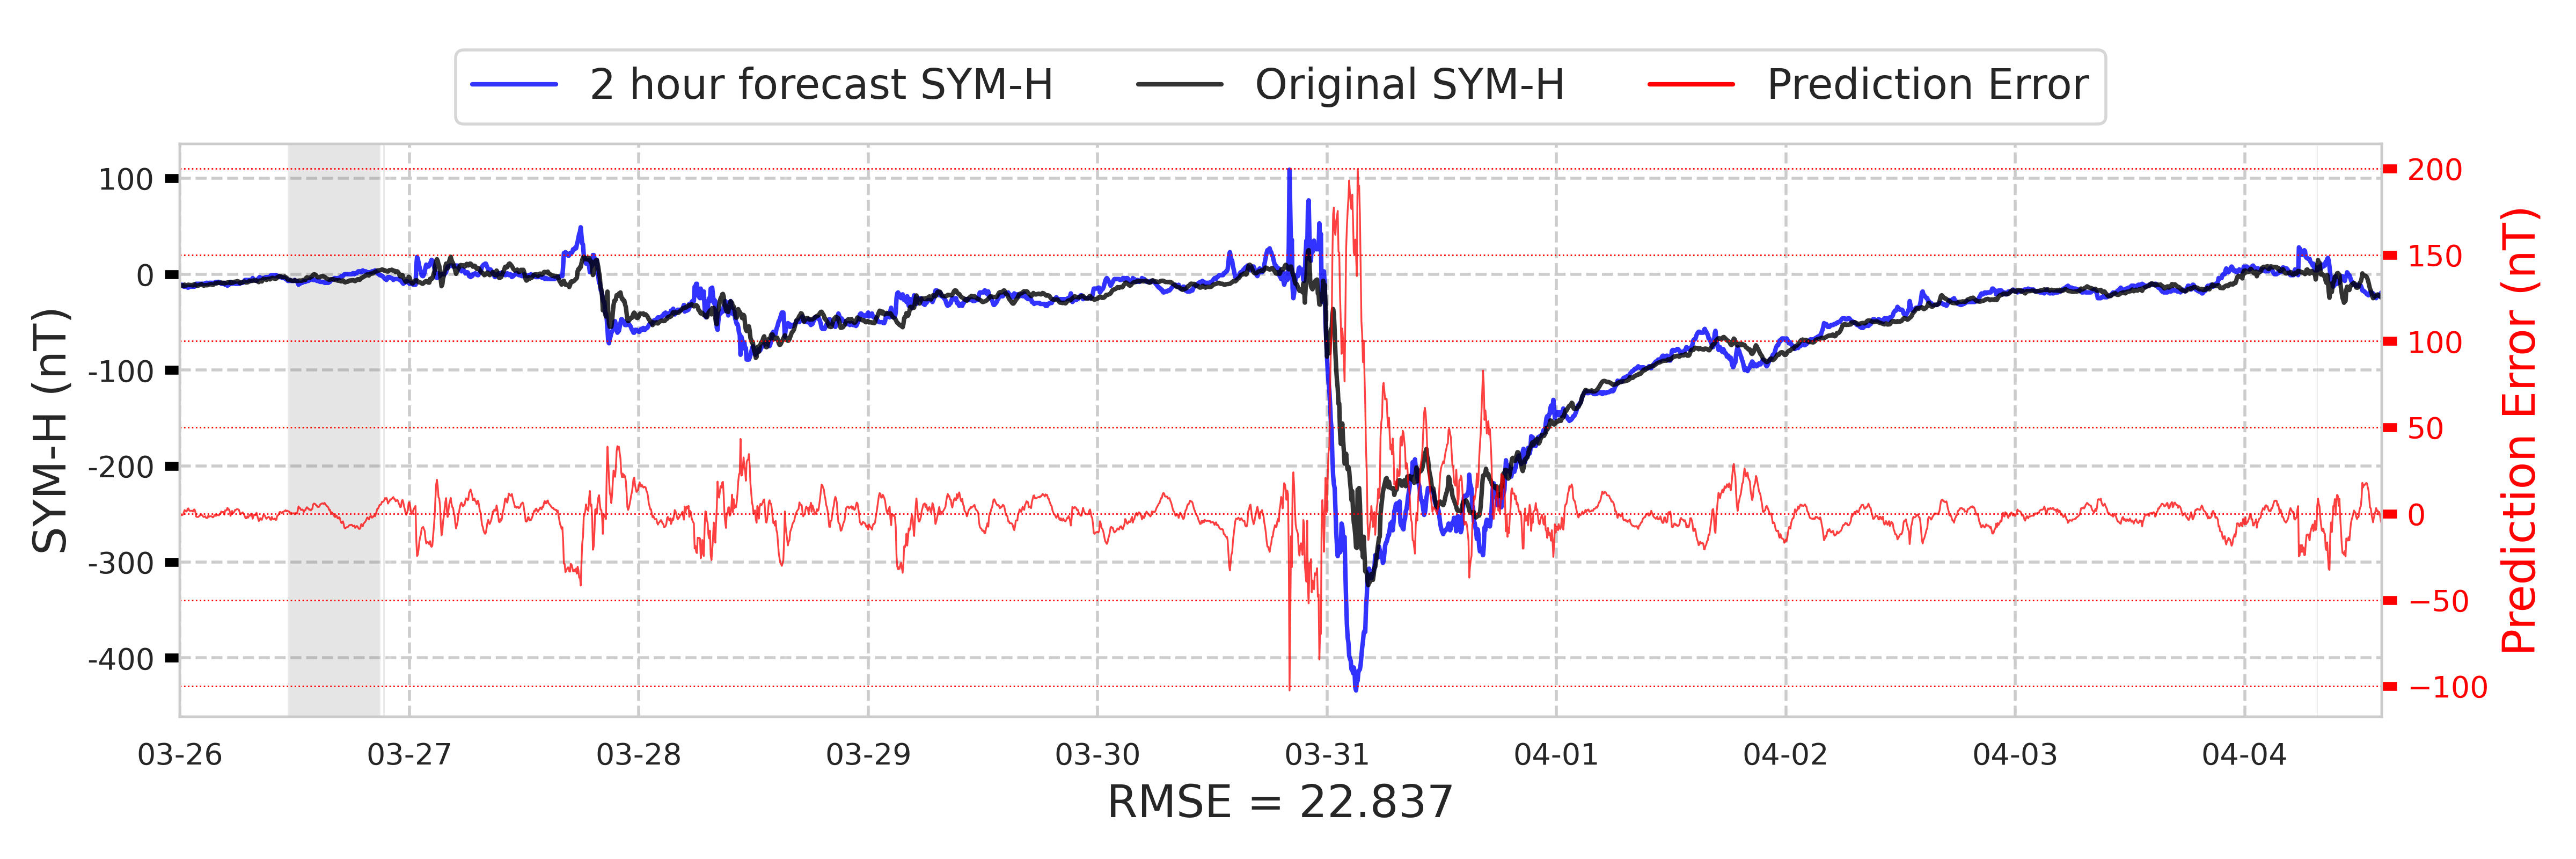
\includegraphics[width=0.49\linewidth]{paper_plots_shade/2h_swepam_rt/2h_swepam_rt_storm_33.png}
\\
\shortstack{1h operational forecast trained\\ with SWEPAM data only} & \shortstack{2h operational forecast trained\\ with SWEPAM data only}
\vspace*{12pt}
\\
\end{tabular}
\caption{Predictions for Storm Number 33 -- March of 2001}
\label{storm-33}
\end{table}



% Figure for storm 34
\begin{table}
\centering
\begin{tabular}{cc}
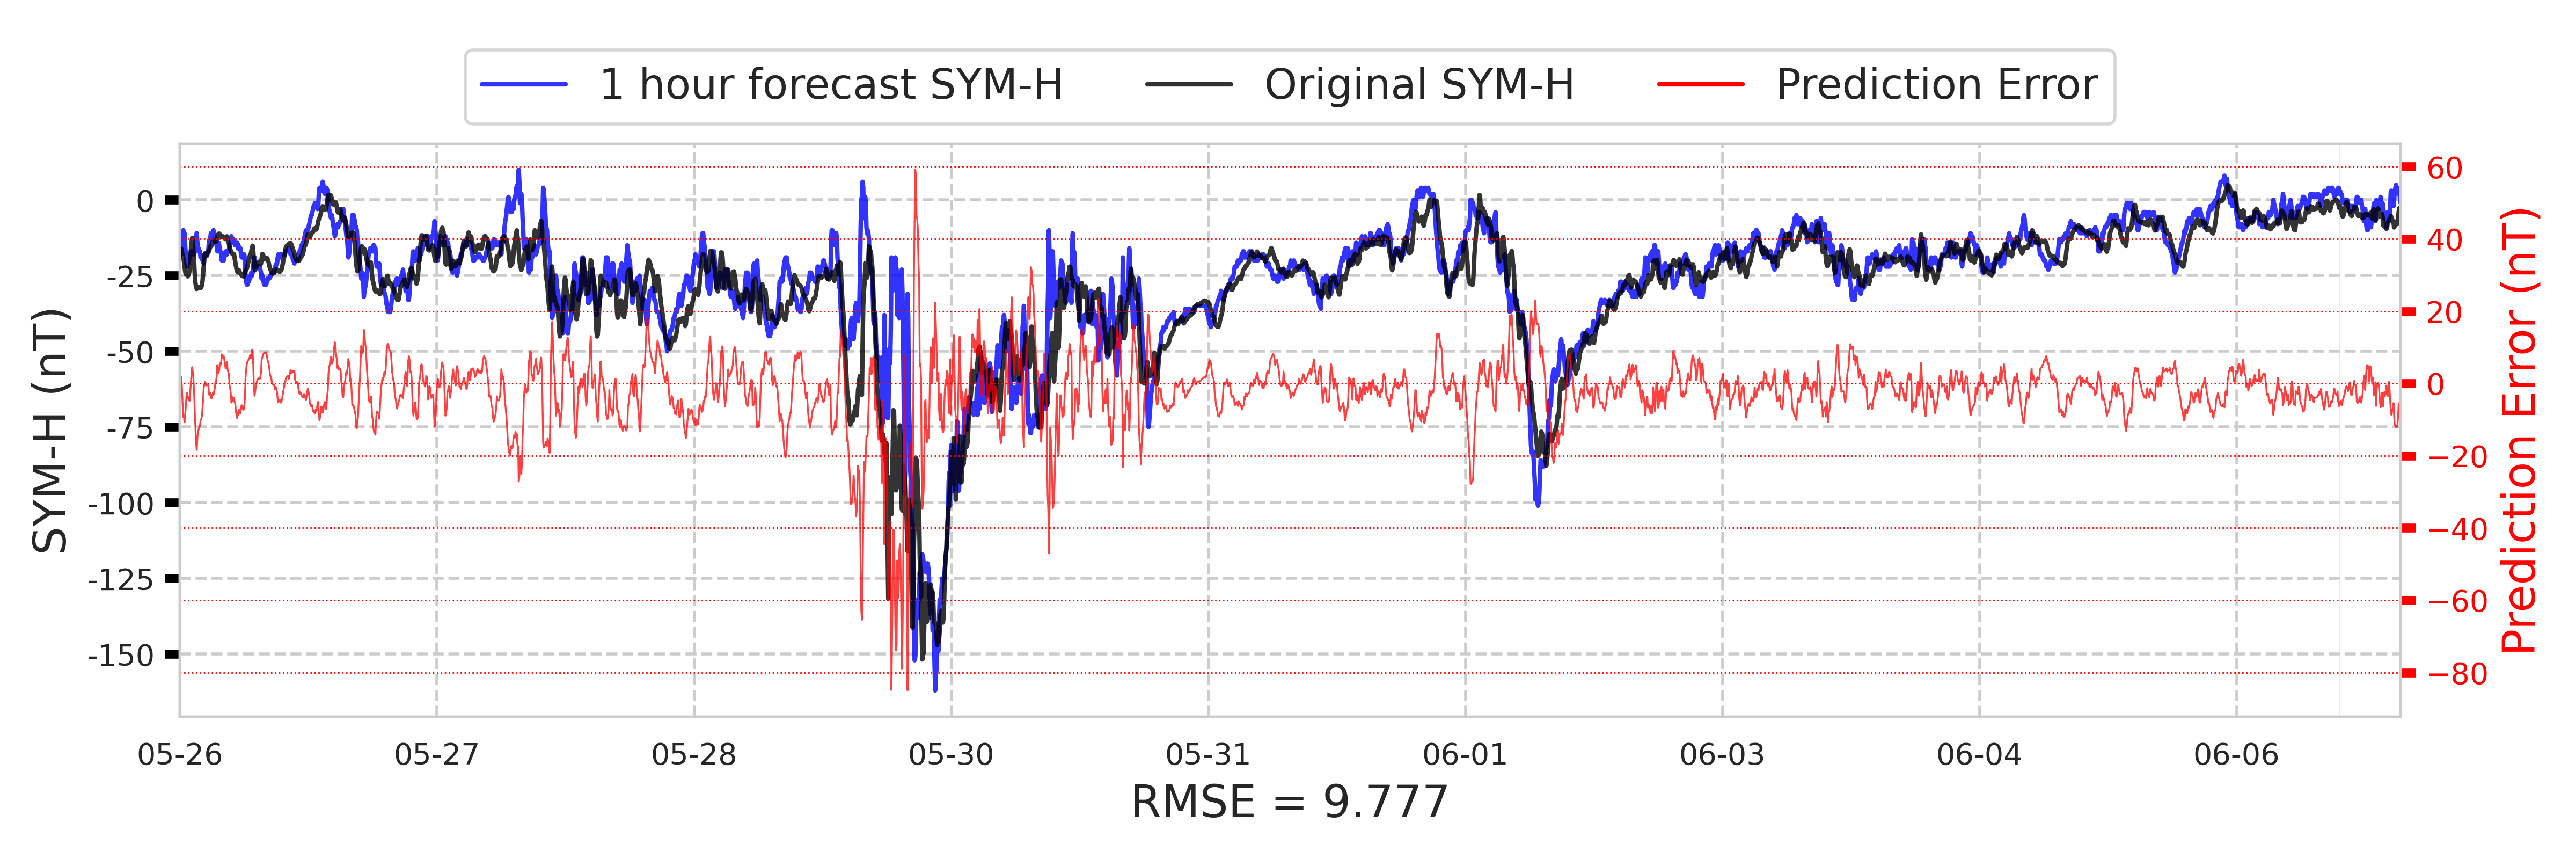
\includegraphics[width=0.49\linewidth]{paper_plots_shade/1h_swics/1h_swics_storm_34.png}
&
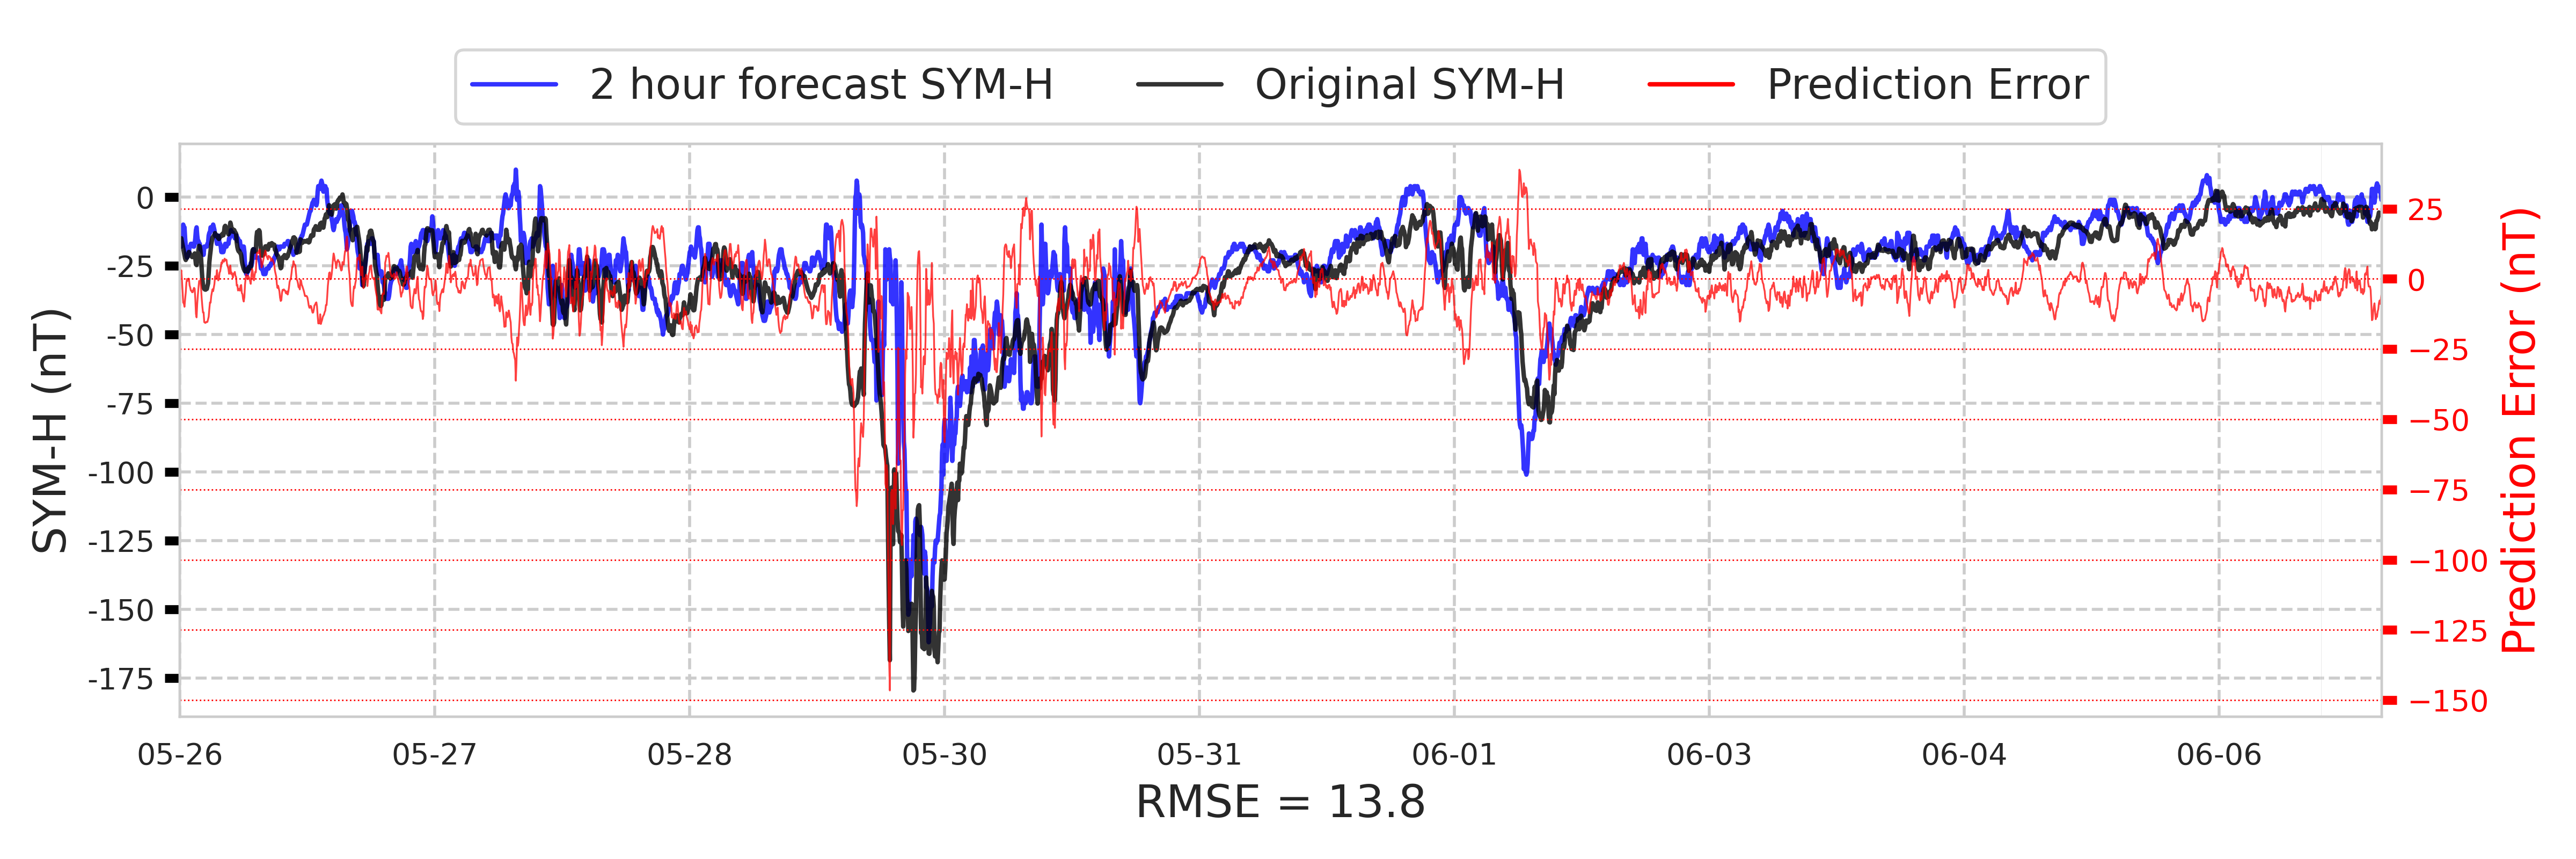
\includegraphics[width=0.49\linewidth]{paper_plots_shade/2h_swics/2h_swics_storm_34.png}
\\
\shortstack{1h forecast using SWICS\\ in laboratory conditions} & \shortstack{2h forecast using SWICS\\ in laboratory conditions}
\vspace*{12pt}
\\
\includegraphics[width=0.49\linewidth]{paper_plots_shade/1h_swics_rt/1h_swics_rt_storm_34.png}
&
\includegraphics[width=0.49\linewidth]{paper_plots_shade/2h_swics_rt/2h_swics_rt_storm_34.png}
\\
\shortstack{1h operational forecast trained\\ with SWEPAM and SWICS data} & \shortstack{2h operational forecast trained\\ with SWEPAM and SWICS data}
\vspace*{12pt}
\\
\includegraphics[width=0.49\linewidth]{paper_plots_shade/1h_swepam_rt/1h_swepam_rt_storm_34.png}
&
\includegraphics[width=0.49\linewidth]{paper_plots_shade/2h_swepam_rt/2h_swepam_rt_storm_34.png}
\\
\shortstack{1h operational forecast trained\\ with SWEPAM data only} & \shortstack{2h operational forecast trained\\ with SWEPAM data only}
\vspace*{12pt}
\\
\end{tabular}
\caption{Predictions for Storm Number 34 -- June of 2003}
\label{storm-34}
\end{table}



% Figure for storm 35
\begin{table}
\centering
\begin{tabular}{cc}
\includegraphics[width=0.49\linewidth]{paper_plots_shade/1h_swics/1h_swics_storm_35.png}
&
\includegraphics[width=0.49\linewidth]{paper_plots_shade/2h_swics/2h_swics_storm_35.png}
\\
\shortstack{1h forecast using SWICS\\ in laboratory conditions} & \shortstack{2h forecast using SWICS\\ in laboratory conditions}
\vspace*{12pt}
\\
\includegraphics[width=0.49\linewidth]{paper_plots_shade/1h_swics_rt/1h_swics_rt_storm_35.png}
&
\includegraphics[width=0.49\linewidth]{paper_plots_shade/2h_swics_rt/2h_swics_rt_storm_35.png}
\\
\shortstack{1h operational forecast trained\\ with SWEPAM and SWICS data} & \shortstack{2h operational forecast trained\\ with SWEPAM and SWICS data}
\vspace*{12pt}
\\
\includegraphics[width=0.49\linewidth]{paper_plots_shade/1h_swepam_rt/1h_swepam_rt_storm_35.png}
&
\includegraphics[width=0.49\linewidth]{paper_plots_shade/2h_swepam_rt/2h_swepam_rt_storm_35.png}
\\
\shortstack{1h operational forecast trained\\ with SWEPAM data only} & \shortstack{2h operational forecast trained\\ with SWEPAM data only}
\vspace*{12pt}
\\
\end{tabular}
\caption{Predictions for Storm Number 35 -- July of 2003}
\label{storm-35}
\end{table}



% Figure for storm 36
\begin{table}
\centering
\begin{tabular}{cc}
\includegraphics[width=0.49\linewidth]{paper_plots_shade/1h_swics/1h_swics_storm_36.png}
&
\includegraphics[width=0.49\linewidth]{paper_plots_shade/2h_swics/2h_swics_storm_36.png}
\\
\shortstack{1h forecast using SWICS\\ in laboratory conditions} & \shortstack{2h forecast using SWICS\\ in laboratory conditions}
\vspace*{12pt}
\\
\includegraphics[width=0.49\linewidth]{paper_plots_shade/1h_swics_rt/1h_swics_rt_storm_36.png}
&
\includegraphics[width=0.49\linewidth]{paper_plots_shade/2h_swics_rt/2h_swics_rt_storm_36.png}
\\
\shortstack{1h operational forecast trained\\ with SWEPAM and SWICS data} & \shortstack{2h operational forecast trained\\ with SWEPAM and SWICS data}
\vspace*{12pt}
\\
\includegraphics[width=0.49\linewidth]{paper_plots_shade/1h_swepam_rt/1h_swepam_rt_storm_36.png}
&
\includegraphics[width=0.49\linewidth]{paper_plots_shade/2h_swepam_rt/2h_swepam_rt_storm_36.png}
\\
\shortstack{1h operational forecast trained\\ with SWEPAM data only} & \shortstack{2h operational forecast trained\\ with SWEPAM data only}
\vspace*{12pt}
\\
\end{tabular}
\caption{Predictions for Storm Number 36 -- January of 2004}
\label{storm-36}
\end{table}



% Figure for storm 37
\begin{table}
\centering
\begin{tabular}{cc}
\includegraphics[width=0.49\linewidth]{paper_plots_shade/1h_swics/1h_swics_storm_37.png}
&
\includegraphics[width=0.49\linewidth]{paper_plots_shade/2h_swics/2h_swics_storm_37.png}
\\
\shortstack{1h forecast using SWICS\\ in laboratory conditions} & \shortstack{2h forecast using SWICS\\ in laboratory conditions}
\vspace*{12pt}
\\
\includegraphics[width=0.49\linewidth]{paper_plots_shade/1h_swics_rt/1h_swics_rt_storm_37.png}
&
\includegraphics[width=0.49\linewidth]{paper_plots_shade/2h_swics_rt/2h_swics_rt_storm_37.png}
\\
\shortstack{1h operational forecast trained\\ with SWEPAM and SWICS data} & \shortstack{2h operational forecast trained\\ with SWEPAM and SWICS data}
\vspace*{12pt}
\\
\includegraphics[width=0.49\linewidth]{paper_plots_shade/1h_swepam_rt/1h_swepam_rt_storm_37.png}
&
\includegraphics[width=0.49\linewidth]{paper_plots_shade/2h_swepam_rt/2h_swepam_rt_storm_37.png}
\\
\shortstack{1h operational forecast trained\\ with SWEPAM data only} & \shortstack{2h operational forecast trained\\ with SWEPAM data only}
\vspace*{12pt}
\\
\end{tabular}
\caption{Predictions for Storm Number 37 -- November of 2004}
\label{storm-37}
\end{table}



% Figure for storm 38
\begin{table}
\centering
\begin{tabular}{cc}
\includegraphics[width=0.49\linewidth]{paper_plots_shade/1h_swics/1h_swics_storm_38.png}
&
\includegraphics[width=0.49\linewidth]{paper_plots_shade/2h_swics/2h_swics_storm_38.png}
\\
\shortstack{1h forecast using SWICS\\ in laboratory conditions} & \shortstack{2h forecast using SWICS\\ in laboratory conditions}
\vspace*{12pt}
\\
\includegraphics[width=0.49\linewidth]{paper_plots_shade/1h_swics_rt/1h_swics_rt_storm_38.png}
&
\includegraphics[width=0.49\linewidth]{paper_plots_shade/2h_swics_rt/2h_swics_rt_storm_38.png}
\\
\shortstack{1h operational forecast trained\\ with SWEPAM and SWICS data} & \shortstack{2h operational forecast trained\\ with SWEPAM and SWICS data}
\vspace*{12pt}
\\
\includegraphics[width=0.49\linewidth]{paper_plots_shade/1h_swepam_rt/1h_swepam_rt_storm_38.png}
&
\includegraphics[width=0.49\linewidth]{paper_plots_shade/2h_swepam_rt/2h_swepam_rt_storm_38.png}
\\
\shortstack{1h operational forecast trained\\ with SWEPAM data only} & \shortstack{2h operational forecast trained\\ with SWEPAM data only}
\vspace*{12pt}
\\
\end{tabular}
\caption{Predictions for Storm Number 38 -- September of 2012}
\label{storm-38}
\end{table}



% Figure for storm 39
\begin{table}
\centering
\begin{tabular}{cc}
\includegraphics[width=0.49\linewidth]{paper_plots_shade/1h_swics/1h_swics_storm_39.png}
&
\includegraphics[width=0.49\linewidth]{paper_plots_shade/2h_swics/2h_swics_storm_39.png}
\\
\shortstack{1h forecast using SWICS\\ in laboratory conditions} & \shortstack{2h forecast using SWICS\\ in laboratory conditions}
\vspace*{12pt}
\\
\includegraphics[width=0.49\linewidth]{paper_plots_shade/1h_swics_rt/1h_swics_rt_storm_39.png}
&
\includegraphics[width=0.49\linewidth]{paper_plots_shade/2h_swics_rt/2h_swics_rt_storm_39.png}
\\
\shortstack{1h operational forecast trained\\ with SWEPAM and SWICS data} & \shortstack{2h operational forecast trained\\ with SWEPAM and SWICS data}
\vspace*{12pt}
\\
\includegraphics[width=0.49\linewidth]{paper_plots_shade/1h_swepam_rt/1h_swepam_rt_storm_39.png}
&
\includegraphics[width=0.49\linewidth]{paper_plots_shade/2h_swepam_rt/2h_swepam_rt_storm_39.png}
\\
\shortstack{1h operational forecast trained\\ with SWEPAM data only} & \shortstack{2h operational forecast trained\\ with SWEPAM data only}
\vspace*{12pt}
\\
\end{tabular}
\caption{Predictions for Storm Number 39 -- June of 2013}
\label{storm-39}
\end{table}



% Figure for storm 40
\begin{table}
\centering
\begin{tabular}{cc}
\includegraphics[width=0.49\linewidth]{paper_plots_shade/1h_swics/1h_swics_storm_40.png}
&
\includegraphics[width=0.49\linewidth]{paper_plots_shade/2h_swics/2h_swics_storm_40.png}
\\
\shortstack{1h forecast using SWICS\\ in laboratory conditions} & \shortstack{2h forecast using SWICS\\ in laboratory conditions}
\vspace*{12pt}
\\
\includegraphics[width=0.49\linewidth]{paper_plots_shade/1h_swics_rt/1h_swics_rt_storm_40.png}
&
\includegraphics[width=0.49\linewidth]{paper_plots_shade/2h_swics_rt/2h_swics_rt_storm_40.png}
\\
\shortstack{1h operational forecast trained\\ with SWEPAM and SWICS data} & \shortstack{2h operational forecast trained\\ with SWEPAM and SWICS data}
\vspace*{12pt}
\\
\includegraphics[width=0.49\linewidth]{paper_plots_shade/1h_swepam_rt/1h_swepam_rt_storm_40.png}
&
\includegraphics[width=0.49\linewidth]{paper_plots_shade/2h_swepam_rt/2h_swepam_rt_storm_40.png}
\\
\shortstack{1h operational forecast trained\\ with SWEPAM data only} & \shortstack{2h operational forecast trained\\ with SWEPAM data only}
\vspace*{12pt}
\\
\end{tabular}
\caption{Predictions for Storm Number 40 -- June of 2013}
\label{storm-40}
\end{table}



% Figure for storm 41
\begin{table}
\centering
\begin{tabular}{cc}
\includegraphics[width=0.49\linewidth]{paper_plots_shade/1h_swics/1h_swics_storm_41.png}
&
\includegraphics[width=0.49\linewidth]{paper_plots_shade/2h_swics/2h_swics_storm_41.png}
\\
\shortstack{1h forecast using SWICS\\ in laboratory conditions} & \shortstack{2h forecast using SWICS\\ in laboratory conditions}
\vspace*{12pt}
\\
\includegraphics[width=0.49\linewidth]{paper_plots_shade/1h_swics_rt/1h_swics_rt_storm_41.png}
&
\includegraphics[width=0.49\linewidth]{paper_plots_shade/2h_swics_rt/2h_swics_rt_storm_41.png}
\\
\shortstack{1h operational forecast trained\\ with SWEPAM and SWICS data} & \shortstack{2h operational forecast trained\\ with SWEPAM and SWICS data}
\vspace*{12pt}
\\
\includegraphics[width=0.49\linewidth]{paper_plots_shade/1h_swepam_rt/1h_swepam_rt_storm_41.png}
&
\includegraphics[width=0.49\linewidth]{paper_plots_shade/2h_swepam_rt/2h_swepam_rt_storm_41.png}
\\
\shortstack{1h operational forecast trained\\ with SWEPAM data only} & \shortstack{2h operational forecast trained\\ with SWEPAM data only}
\vspace*{12pt}
\\
\end{tabular}
\caption{Predictions for Storm Number 41 -- March of 2015}
\label{storm-41}
\end{table}



% Figure for storm 42
\begin{table}
\centering
\begin{tabular}{cc}
\includegraphics[width=0.49\linewidth]{paper_plots_shade/1h_swics/1h_swics_storm_42.png}
&
\includegraphics[width=0.49\linewidth]{paper_plots_shade/2h_swics/2h_swics_storm_42.png}
\\
\shortstack{1h forecast using SWICS\\ in laboratory conditions} & \shortstack{2h forecast using SWICS\\ in laboratory conditions}
\vspace*{12pt}
\\
\includegraphics[width=0.49\linewidth]{paper_plots_shade/1h_swics_rt/1h_swics_rt_storm_42.png}
&
\includegraphics[width=0.49\linewidth]{paper_plots_shade/2h_swics_rt/2h_swics_rt_storm_42.png}
\\
\shortstack{1h operational forecast trained\\ with SWEPAM and SWICS data} & \shortstack{2h operational forecast trained\\ with SWEPAM and SWICS data}
\vspace*{12pt}
\\
\includegraphics[width=0.49\linewidth]{paper_plots_shade/1h_swepam_rt/1h_swepam_rt_storm_42.png}
&
\includegraphics[width=0.49\linewidth]{paper_plots_shade/2h_swepam_rt/2h_swepam_rt_storm_42.png}
\\
\shortstack{1h operational forecast trained\\ with SWEPAM data only} & \shortstack{2h operational forecast trained\\ with SWEPAM data only}
\vspace*{12pt}
\\
\end{tabular}
\caption{Predictions for Storm Number 42 -- August of 2018}
\label{storm-42}
\end{table}




\end{document}